% ==================== 研报 V2 专用 pandoc 模板（卖方研报风格 · 红色主题） ====================
\documentclass[UTF8,a4paper,zihao=-4,fontset=windows]{ctexart}

% ---------- 页边距（压缩留白） ----------
\usepackage[a4paper,top=2.0cm,bottom=2.0cm,left=1.9cm,right=1.9cm]{geometry}

% ---------- 常用宏包 ----------
\usepackage{amsmath,amssymb}
\usepackage{calc}
\usepackage{booktabs}
\usepackage{longtable}
\usepackage{array}
\usepackage{multirow}
\usepackage{caption}
\usepackage{float}
\usepackage{graphicx}
\usepackage{xcolor}
\usepackage{etoolbox}
\usepackage{fancyhdr}
\usepackage{tcolorbox}
\usepackage{hyperref}
\usepackage{newunicodechar}
\newunicodechar{↔}{\ensuremath{\leftrightarrow}}
\newunicodechar{∧}{\ensuremath{\land}}
\newunicodechar{≤}{\ensuremath{\leq}}
\newunicodechar{≈}{\ensuremath{\approx}}
\newunicodechar{β}{\ensuremath{\beta}}
\newunicodechar{①}{1.}
\newunicodechar{②}{2.}
\newunicodechar{③}{3.}
\newunicodechar{④}{4.}
\newunicodechar{⑤}{5.}
\newunicodechar{⑥}{6.}
\newunicodechar{⑦}{7.}

% ---------- 配色（红色主题） ----------
\definecolor{reportred}{RGB}{180,0,0}
\definecolor{reportgray}{RGB}{246,246,246}

% ---------- 超链接 / 书签 ----------
\hypersetup{
  colorlinks=true, linkcolor=reportred, urlcolor=reportred,
  bookmarks=true, bookmarksnumbered=true,
  pdftitle={高频因子：收益来源基础的因子挖掘方法论——路径形态、量价交互与时序分布因子},
}

% ---------- 页眉页脚（金融工程深度报告风格，红色分隔线） ----------
\pagestyle{fancy}
\fancyhf{}
\fancyhead[L]{\small\heiti 金融工程｜深度报告}
\fancyhead[R]{\small 高频因子｜收益来源基础的因子挖掘方法论}
\fancyfoot[C]{\small\thepage}
\setlength{\headheight}{24pt}
\renewcommand{\headrulewidth}{0.5pt}
\renewcommand{\headrule}{\hbox to\headwidth{\color{reportred}\leaders\hrule height \headrulewidth\hfill}}

% ---------- 表格样式：small + 紧凑列距 + booktabs ----------
\setlength{\tabcolsep}{5pt}
\renewcommand{\arraystretch}{1.15}
\BeforeBeginEnvironment{longtable}{\small}
\BeforeBeginEnvironment{tabular}{\small}
% 表注：去掉自动"表 N"前缀（用预处理注入的手工编号），字体小号、居中（longtable 默认居中）
\captionsetup[longtable]{font=small,labelformat=empty}

% ---------- 标题层级（md 已含手工编号，关闭自动编号；压缩间距减少留白） ----------
\ctexset{
  section = { format = {\Large\bfseries\heiti\textcolor{reportred}}, numbering = false, beforeskip = 14pt, afterskip = 6pt },
  subsection = { format = {\large\bfseries\heiti}, numbering = false, beforeskip = 10pt, afterskip = 4pt },
}

% ---------- 目录深度 ----------
\setcounter{tocdepth}{2}

% ---------- 图片默认宽度 ----------
\graphicspath{{figs_v21/}{figs/}}

% ---------- pandoc 自定义模板缺省的辅助宏 ----------
\providecommand{\tightlist}{\setlength{\itemsep}{0pt}\setlength{\parskip}{0pt}}
\providecommand{\pandocbounded}[1]{\makebox[1.1\linewidth][c]{#1}}
% 宽松断行容差，减少末行轻微溢出
\emergencystretch=2em

\begin{document}
\begin{titlepage}
\centering
\vspace*{1.8cm}
\begin{minipage}{0.98\textwidth}
\centering
{\fontsize{20.5pt}{30pt}\selectfont\bfseries\heiti\textcolor{reportred}{高频因子：收益来源基础的因子挖掘方法论}}\\[14pt]
{\fontsize{16pt}{26pt}\selectfont\heiti\color{black!78} ——路径形态、量价交互与时序分布因子}
\end{minipage}\\[18pt]
\textcolor{reportred}{\rule{0.64\textwidth}{1pt}}\\[14pt]
{\small\color{black!60} 研究区间：2016-07 \textasciitilde{} 2026-06（120 个形成月）　|　数据：全市场 1 分钟 K 线（2004-01 \textasciitilde{} 2026-07）\\[3pt]股票池：沪深300 / 中证500 / 中证1000 / 中证全指　|　因子体系：3 模块、18 因子\\[3pt]回测组合：4 池 × 18 因子 × 2 中性化方案 = 144 组　|　调仓：月度、单边千三}\\[22pt]
\vfill
\begin{flushright}
\begin{minipage}{0.34\textwidth}
\raggedleft
\textcolor{reportred}{\rule{\linewidth}{0.8pt}}\\[9pt]
{\large\heiti\color{black!85} 胡智超}\\[7pt]
{\small\color{black!55} 金融工程深度研究报告}\\[4pt]
{\small\color{black!55} 2026 年 8 月}
\end{minipage}
\end{flushright}
\vspace*{1.2cm}
\end{titlepage}
\tableofcontents
\newpage

\begin{tcolorbox}[colback=reportred,coltext=white,boxrule=0pt,left=8pt,right=8pt,top=5pt,bottom=5pt]
{\Large\bfseries\heiti 报告要点}
\end{tcolorbox}

本文以''\textbf{数据变换---K
线聚合}''的统一算子语法，将日内价格路径的\textbf{形态}信息（而非仅涨跌幅）刻画为三个互补模块------微观结构（价格路径质量）、时序特征（量价交互方向）、成交时序集中度（信息到达模式）------共
18
个可解释算子链因子，在十年期、四个股票池、市值行业中性（S1）与量价中性（S2）两套口径下完成
144 组回测。主要结论如下：

\begin{enumerate}
\def\labelenumi{\arabic{enumi}.}
\tightlist
\item
  \textbf{路径形态的''结构''信息优于''总量''信息。} 基础曲折度 A1
  全池偏弱（中证1000 RankICIR 仅
  0.41），而经时段切割并与放量交叉后，A3（曲折放量共振）与
  A2c（高曲折时段成交集中度）成为全体系最强因子：A3 在中证全指 RankIC
  9.32\%、RankICIR 3.53、毛多空年化 +24.6\%；A2c
  在四个股票池全部显著（RankICIR
  1.63\textasciitilde3.36）。这印证了''日内定价效率具有时变结构、噪音交易集中在高曲折放量时段''的微观结构叙事。
\item
  \textbf{量价交互的''方向性''信息真实存在，但分布不均。}
  刻画''顶背离''的
  B5c（价格新高量能不足）方向稳定为负（中证1000/中证全指 RankICIR
  −3.34/−3.71，创新高缩量者未来跑输），且全部 9
  个完整年份同向；量价领先滞后 B1 在小盘池有效（RankICIR
  1.34/1.44）、在沪深300 失效；而''上行 vs
  下行力量对比''（B2/B2a）与''量价趋势斜率背离''（B5b）在月度频率上基本无效------``先后''与''极值点''维度携带信息，``上下力量对比''维度信息有限。
\item
  \textbf{买卖盘集中度差异 C2 是体系中最干净的增量。} C2
  在四个股票池全部显著（RankICIR
  1.19\textasciitilde2.55），且量价中性后衰减最小（沪深300
  1.19→0.97）；集中度的''水平''（C1）与''波动''（C3）信息有限，说明''买卖两盘的相对分布''才携带主力行为信息。
\item
  \textbf{量价中性化是增量试金石，也是本体系的主要软肋；补全九风格后信号反而更稳。}
  在市值行业中性之上再剥离换手率与波动率（S2）后，A3/A2c 的 RankICIR
  约打对折（中证1000 A3：3.30→1.83）------模块 A
  的收益来源有相当部分''借自''波动率与换手率暴露，与低波/低换手异象同源，入组合时必须按暴露管理。\textbf{在进一步补全动量/反转/BP/DP/成长/盈利六风格（S3，九风格全中性）后，各因子几乎不再衰减}（中证全指
  A3 2.16→2.15、A2c 1.86→1.92、B5c −2.44→−2.38），且 C2/B1 反被修复（C2
  1.66→2.07、B1 0.54→0.98）------模块 A
  的暴露确系''低波/低换手''而非价值/动量/盈利来源，C2/B5c
  在完整九风格中性化后仍显著（2.07/−2.38），是最接近独立维度的增量。
\item
  \textbf{信号真实，但月度调仓下的可交易性是硬约束。}
  修正权重漂移后的换手计算后，四个股票池的平均单组月换手为
  1.44\textasciitilde1.72，多空双腿月换手为
  2.62\textasciitilde3.10。按全样本两端组合的实际收益确定多空方向，\textbf{扣成本后净多空年化
  \textgreater{} 5\% 的组合共 6 个}，均来自中证1000或中证全指的
  A3、A2c 与 A2d（+6.67\%\textasciitilde+12.87\%）；B5c 在中证1000和中证全指的有效净多空年化修订为 4.32\%和2.02\%。
\item
  \textbf{近期衰减是结构性轮动而非均匀压缩。} A3 在中证1000 的分年 IC 从
  2017-2020 的 4\%\textasciitilde10\% 降至 2024 年 3.6\%、2025 年
  2.0\%、2026 上半年约 0；全部 144
  组的时序衰减分析进一步显示：领先滞后族（B3/B4/B5a）2023
  年后基本消失、A3/A2c 衰减而未失效、C3/A2a
  反向增强------近期子样本监控应成为例行动作。
\end{enumerate}

\begin{center}\rule{0.5\linewidth}{0.5pt}\end{center}

\section{一、研究背景与因子体系设计}\label{ux4e00ux7814ux7a76ux80ccux666fux4e0eux56e0ux5b50ux4f53ux7cfbux8bbeux8ba1}

\subsection{1.1
研究范式背景：从''预测导向''到''收益来源导向''}\label{ux7814ux7a76ux8303ux5f0fux80ccux666fux4eceux9884ux6d4bux5bfcux5411ux5230ux6536ux76caux6765ux6e90ux5bfcux5411}

高频因子研究需要从''预测是否有效''进一步转向''超额从何而来''：收益来源决定组合的风险暴露、收益归因与因子轮动。为此，本研究把每个高频因子拆解为\textbf{数据变换（向量→向量，交易信息的局部处理）与
K
线聚合（向量→标量，交易信息的局部整合/降频）}的嵌套算子链；由于因子最终是个股日度的一个标量，\textbf{最后一步必为
K
线聚合}；高频数据的价值，在于允许''变换↔聚合''反复交叉，在聚合之前先把微观结构信息提炼出来。

本研究在上述范式框架内，引入一个新的信息维度。传统量价因子关注''交易了多少''（成交量/换手率）、``波动了多大''（振幅/波动率）、``涨跌了多少''（收益率），其本质均是对路径的\textbf{统计矩}描述------回答''量级''，而非''\textbf{形态}''。微观结构理论表明，路径形态直接反映交易者行为：\textbf{平滑单调的路径对应信息驱动型交易}（知情者沿单一方向持续建仓），\textbf{剧烈振荡的路径对应噪音/流动性交易}（多空分歧、反复折返）；\textbf{量先于价对应信息渐进扩散}（知情交易先建仓、价格滞后反映），\textbf{价先于量对应情绪追涨}（突破后跟风盘跟进）；\textbf{成交集中于少数时段对应信息脉冲}（事件/大单驱动），\textbf{成交均匀分散对应持续价格发现}。因此，\textbf{两只日收益率、日内波动与成交量完全相同的股票，可能因路径形态不同而具有截然不同的未来收益表现}------这正是''路径形态''作为独立信息切面的价值所在。

\subsection{1.2
因子体系设计：三模块的划分逻辑}\label{ux56e0ux5b50ux4f53ux7cfbux8bbeux8ba1ux4e09ux6a21ux5757ux7684ux5212ux5206ux903bux8f91}

将''日内路径形态''拆解为三个\textbf{互补而非重叠}的研究问题，每个问题对应一个模块、一条收益来源主线：

\begin{longtable}[]{@{}
  >{\raggedright\arraybackslash}p{(\linewidth - 6\tabcolsep) * \real{0.2500}}
  >{\raggedright\arraybackslash}p{(\linewidth - 6\tabcolsep) * \real{0.2500}}
  >{\raggedright\arraybackslash}p{(\linewidth - 6\tabcolsep) * \real{0.2500}}
  >{\raggedright\arraybackslash}p{(\linewidth - 6\tabcolsep) * \real{0.2500}}@{}}
\caption{表 1　三模块设计总览}\tabularnewline
\toprule\noalign{}
\begin{minipage}[b]{\linewidth}\raggedright
模块
\end{minipage} & \begin{minipage}[b]{\linewidth}\raggedright
研究问题
\end{minipage} & \begin{minipage}[b]{\linewidth}\raggedright
核心视角
\end{minipage} & \begin{minipage}[b]{\linewidth}\raggedright
收益来源主标签
\end{minipage} \\
\midrule\noalign{}
\endfirsthead
\toprule\noalign{}
\begin{minipage}[b]{\linewidth}\raggedright
模块
\end{minipage} & \begin{minipage}[b]{\linewidth}\raggedright
研究问题
\end{minipage} & \begin{minipage}[b]{\linewidth}\raggedright
核心视角
\end{minipage} & \begin{minipage}[b]{\linewidth}\raggedright
收益来源主标签
\end{minipage} \\
\midrule\noalign{}
\endhead
\bottomrule\noalign{}
\endlastfoot
\textbf{A 微观结构} & 价格路径如何演化？噪音集中于哪些时段？ &
路径''纹理''与定价效率 & 价格稳定性 / 噪音交易强度 \\
\textbf{B 时序特征} &
量与价孰先孰后？多空力量如何倾斜？趋势有无交易确认？ &
量价交互的时序方向性 & 信息扩散模式 / 拥挤度 / 动量衰竭 \\
\textbf{C 成交时序集中度} & 交易发生于何时？买卖两盘的时间分布有何差异？
& 信息到达的脉冲式与连续式 & 信息到达模式 / 主力行为 \\
\end{longtable}

三模块架构系对初始''五因子并列''方案的整合修订：路径曲折度（价格维度）与路径时段切割（结构维度）同属''价格路径质量''，归并至模块
A；量价领先滞后（先后）与路径不对称性（上下）均为量价时序交互的不同切面，归并至模块
B；成交时序集中度（何时交易）与路径形状、量价方向均正交，独立成模块
C。归并后，各模块内部形成''\textbf{总量 → 结构 →
交叉}''的递进关系，且每个模块均\textbf{强制价格与成交量两个维度同时参与}（综合量价原则）：模块
A 在切割后同时提取收益率（价）与成交占比/换手（量），模块 B
全部采用量价联合算子，模块 C 在熵的基础上引入价格方向条件化（C2）。

\subsection{1.3
统一算子语法与离散化谱系定位}\label{ux7edfux4e00ux7b97ux5b50ux8bedux6cd5ux4e0eux79bbux6563ux5316ux8c31ux7cfbux5b9aux4f4d}

全部 18
个因子均以显式算子链表达，每个算子具有逻辑含义，因子自构建起即可确定其收益来源归属。按信息定位精度，可把日内离散化概括为''\textbf{整体聚合
→ 阈值时间段切割 →
极值时间点划分}''：整体聚合保留全日总量，时间段切割隔离不同经济状态，时间点划分以极值事件为锚提取局部状态。本体系覆盖前两级并触及第三级：

\begin{itemize}
\tightlist
\item
  \textbf{整体聚合（离散向量为
  \(\vec{1}\)）}：A1、C1、B5b------单维度总量，信噪比最低，实证亦最弱；
\item
  \textbf{阈值/条件时间段切割}：A2（按滚动曲折度切分高/低曲折时段）、A3（高曲折∧放量的且逻辑）、C2（按价格方向切分上涨/下跌分钟）、B3（按涨跌条件化相关）------以离散条件向量筛选连续量价向量；
\item
  \textbf{极值时间点锚定}：B5c（以累计收益新高时刻为锚统计量能）------先定位稀疏事件，再对锚点与非锚点状态做对照。
\end{itemize}

该谱系安排并非形式安排，而是给出一个\textbf{可检验的预测：切割应带来增量，且增量大小取决于''切割条件能否分离相反逻辑''}。实证结果基本验证该预测（A1→A2/A3、C1→C2
的跃升），亦给出反例（B2''上下切割''无效，见 3.4 节）。

\subsection{1.4
数据说明与回测设置}\label{ux6570ux636eux8bf4ux660eux4e0eux56deux6d4bux8bbeux7f6e}

\textbf{数据说明：}

\begin{longtable}[]{@{}
  >{\raggedright\arraybackslash}p{(\linewidth - 6\tabcolsep) * \real{0.2500}}
  >{\raggedright\arraybackslash}p{(\linewidth - 6\tabcolsep) * \real{0.2500}}
  >{\raggedright\arraybackslash}p{(\linewidth - 6\tabcolsep) * \real{0.2500}}
  >{\raggedright\arraybackslash}p{(\linewidth - 6\tabcolsep) * \real{0.2500}}@{}}
\caption{表 2　数据说明}\tabularnewline
\toprule\noalign{}
\begin{minipage}[b]{\linewidth}\raggedright
数据
\end{minipage} & \begin{minipage}[b]{\linewidth}\raggedright
内容
\end{minipage} & \begin{minipage}[b]{\linewidth}\raggedright
覆盖
\end{minipage} & \begin{minipage}[b]{\linewidth}\raggedright
用途
\end{minipage} \\
\midrule\noalign{}
\endfirsthead
\toprule\noalign{}
\begin{minipage}[b]{\linewidth}\raggedright
数据
\end{minipage} & \begin{minipage}[b]{\linewidth}\raggedright
内容
\end{minipage} & \begin{minipage}[b]{\linewidth}\raggedright
覆盖
\end{minipage} & \begin{minipage}[b]{\linewidth}\raggedright
用途
\end{minipage} \\
\midrule\noalign{}
\endhead
\bottomrule\noalign{}
\endlastfoot
1 分钟 K 线 & OHLCV、成交额、五档量价、复权因子 & 2004-01
\textasciitilde{} 2026-07，5482 个交易日 & 因子构建核心输入 \\
全 A 日线 & 后复权收盘、换手率、流通市值、涨跌停/ST 标记、申万一级行业 &
2002 \textasciitilde{} 2026-07 & 中性化、可交易性过滤 \\
指数成分权重 & 沪深300/中证500/中证1000/中证全指 日频时点权重 &
含历史调入调出 & 分池回测、避免幸存者偏差 \\
\end{longtable}

\textbf{回测设置}（与月度调仓、t1 收盘建仓的行业标准对齐）：

\begin{itemize}
\tightlist
\item
  \textbf{建仓时点}：因子使用 ≤ t 的全部信息（含 t
  日全天分钟数据），\textbf{建仓日 t1 = 次一交易日、按 t1
  收盘价建仓}，持有至下月末结算------信号时点与成交时点严格分离；
\item
  \textbf{股票池}：成分按形成日 t
  的时点权重选取（含历史调入调出），无幸存者偏差；
\item
  \textbf{可交易性}：剔除 ST、上市不足 60 个交易日、建仓日 t1
  涨跌停/停牌、形成月内停牌超 5 天的样本；空值直接剔除，极端值按 5 倍
  MAD 直接删除；
\item
  \textbf{中性化}：S1 = 对数流通市值 +
  申万一级行业哑变量施密特正交化取残差；S2 = S1 + 21 日换手率 + 21
  日波动率。S1→S2 的 RankICIR
  落差度量''收益来源中借自波动率/换手率的部分''，为本研究的增量试金石；
\item
  \textbf{分组与成本}：沪深300/中证500 分五组、中证1000/中证全指
  分十组，组内等权持有一个月；单边千三按换手 \(\sum|\Delta w|\)
  逐月扣减；多头腿 = 高因子组 \(G_N\)、空头腿 = 低因子组
  \(G_1\)，多空收益 = \(G_N-G_1\)（符号与 IC
  一致）；毛多空展示信号纯度，净多空展示可交易性。
\end{itemize}

\subsection{1.5
符号约定（全文统一）}\label{ux7b26ux53f7ux7ea6ux5b9aux5168ux6587ux7edfux4e00}

\begin{longtable}[]{@{}
  >{\raggedright\arraybackslash}p{(\linewidth - 2\tabcolsep) * \real{0.5000}}
  >{\raggedright\arraybackslash}p{(\linewidth - 2\tabcolsep) * \real{0.5000}}@{}}
\caption{表 3　符号约定（全文统一）}\tabularnewline
\toprule\noalign{}
\begin{minipage}[b]{\linewidth}\raggedright
符号
\end{minipage} & \begin{minipage}[b]{\linewidth}\raggedright
含义
\end{minipage} \\
\midrule\noalign{}
\endfirsthead
\toprule\noalign{}
\begin{minipage}[b]{\linewidth}\raggedright
符号
\end{minipage} & \begin{minipage}[b]{\linewidth}\raggedright
含义
\end{minipage} \\
\midrule\noalign{}
\endhead
\bottomrule\noalign{}
\endlastfoot
\(C_t,\ H_t,\ L_t\) & 第 t 分钟收盘价、最高价、最低价 \\
\(V_t\) & 第 t 分钟成交量 \\
\(r_t=\ln(C_t/C_{t-1})\) & 分钟对数收益率（要求相邻两分钟收盘均有效） \\
\(a_t=(H_t-L_t)/C_{t-1}\) & 分钟振幅（含上下影线信息） \\
\(\Delta v_t=(V_t-V_{t-1})/V_{t-1}\) & 分钟成交量变化率（前量 \(\le0\)
处无定义） \\
\(\Delta V_t=V_t-V_{t-1}\) & 分钟成交量差分 \\
\(w_t=V_t/\sum_s V_s\) & 分钟成交量占全日比重 \\
\(\bar V\) & 有效分钟上的平均成交量 \\
\(\mu_V,\ \sigma_V\) & 日内分钟成交量的均值与标准差 \\
\(T=240\) & 日内分钟数（连续竞价） \\
\(\mathbb{1}\{\cdot\}\) & 示性函数（条件成立取 1，否则取 0） \\
\(\varepsilon\) & 防除零小量 \\
\(\mathrm{Corr}(\cdot,\cdot)\) & 相关系数 \\
\(\mathrm{Mean}_{20d}(\cdot)\) & 20 个交易日滚动均值 \\
\(\mathrm{Std}_{20d}(\cdot)\) & 20 个交易日滚动标准差 \\
\(\tau_t^{(30)}\) & 30 分钟滚动曲折度（窗口 \([t-29,t]\)，模块 A） \\
\(d_t\) &
高曲折标记，\(d_t=\mathbb{1}\{\tau_t^{(30)}>\mathrm{Median}(\tau^{(30)})\}\)（模块
A） \\
\(T_{\mathrm{win}}\) & 日内有定义滚动曲折度窗口的个数（模块 A） \\
\(C_{\mathrm{high}}=\sum_{d_t=1}w_t\) & 高曲折时段成交占比（模块 A） \\
\(\mathrm{Turnover}_d\) & 当日换手率（百分数，模块 A） \\
\(P_t=\sum_{s\le t}r_s\) & 日内累计价格路径（模块 B） \\
\(Q_t=\sum_{s\le t}(V_s-\bar V)\) & 日内累计成交量偏离路径（模块 B） \\
\(h_t\) &
累计收益新高标记，\(h_t=\mathbb{1}\{P_t=\max_{s\le t}P_s\}\)（模块
B） \\
\(\rho_{+k},\ \rho_{-k}\) & 量领先价、价领先量的 k 阶滞后相关系数（模块
B） \\
\(\rho_{59},\ \rho_{239}\) & 第 60、第 240 根 bar 处的 60
分钟滚动量价相关（模块 B） \\
\(\hat\beta_p^s,\ \hat\beta_v^s\) & 标准化后的价格、成交量累计路径 OLS
斜率（模块 B） \\
\(H^*\) & 标准化日内成交熵（模块 C） \\
\(w_t^+,\ w_t^-\) & 上涨、下跌分钟的量占比（模块 C） \\
\(H^+,\ H^-\) & 上涨、下跌分钟的成交熵（模块 C） \\
\end{longtable}

\begin{center}\rule{0.5\linewidth}{0.5pt}\end{center}

\section{二、模块
A：微观结构类因子------价格路径质量与时变结构}\label{ux4e8cux6a21ux5757-aux5faeux89c2ux7ed3ux6784ux7c7bux56e0ux5b50ux4ef7ux683cux8defux5f84ux8d28ux91cfux4e0eux65f6ux53d8ux7ed3ux6784}

\subsection{2.1 构建动机}\label{ux6784ux5efaux52a8ux673a}

模块 A
旨在刻画\textbf{日内价格路径是''平滑推进''还是''反复折返''、噪音集中于哪些时段}。经典残差波动率/振幅类因子仅度量''波动有多大''，而''\textbf{到达终点的方式}''携带独立信息：一只股票可能全天跟随市场、残差波动很低，但日内路径极度曲折（噪音交易主导）；另一只股票可能大起大落但方向单一（趋势主导）。据此，模块
A 以\textbf{路径曲折度}为核心锚点，沿''总量 → 时段切割 →
量价交叉''三层递进：

\begin{enumerate}
\def\labelenumi{\arabic{enumi}.}
\tightlist
\item
  \textbf{总量层（A1/A1v）}：度量当日路径整体的''绕路''程度；
\item
  \textbf{结构层（A2a\textasciitilde A2d）}：按滚动曲折度将交易日切分为''高曲折（噪音主导）/低曲折（信息驱动）``两类时段，分别提取噪音强度、信息驱动收益、成交集中度与换手强度；
\item
  \textbf{交叉层（A3）}：考察噪音是否被资金放大------高曲折与放量同时出现的占比，为''定价效率最差状态''的直接刻画。
\end{enumerate}

\subsection{2.2
因子定义与计算方法}\label{ux56e0ux5b50ux5b9aux4e49ux4e0eux8ba1ux7b97ux65b9ux6cd5}

统一记号：\(r_t=\ln(C_t/C_{t-1})\) 为分钟对数收益；\(V_t\)
为分钟成交量；\(w_t=V_t/\sum_s V_s\)
为分钟量占比；\(a_t=(H_t-L_t)/C_{t-1}\) 为分钟振幅；\(T=240\)
为日内分钟数；\(\varepsilon\) 为防除零小量。

本模块按''\textbf{数据变换（向量→向量，交易信息局部处理）→ K
线聚合（向量→标量，交易信息局部整合/降频）}''的算子链逐因子给出计算方法：高频数据的价值正在于允许''变换↔聚合''反复交叉、在聚合前先把微观结构提炼出来，任何因子末端必为
K 线聚合（多为 \textbf{20 日滚动均值}）。

\textbf{公共中间量：30 分钟滚动曲折度与高/低曲折切割}

\begin{enumerate}
\def\labelenumi{\arabic{enumi}.}
\tightlist
\item
  \textbf{数据变换}（时序·对数）：分钟对数收益
  \(r_t=\ln(C_t/C_{t-1})\)；
\item
  \textbf{数据变换}（窗口绝对值/求和）：30 分钟窗口 \([t-29,t]\)
  内路径长度 \(L^{(30)}_t=\sum_{s=t-29}^{t}|r_s|\)、净位移
  \(D^{(30)}_t=\left|\sum_{s=t-29}^{t}r_s\right|\)（29
  个相邻收益全部有效才有定义）；
\item
  \textbf{数据变换}（除法）：30 分钟滚动曲折度
  \(\tau^{(30)}_t=\dfrac{L^{(30)}_t}{D^{(30)}_t+\varepsilon}\)；
\item
  \textbf{K 线聚合}（中位数）：日内切割阈值
  \(\bar\tau=\mathrm{Median}\big(\tau^{(30)}\big)\)；
\item
  \textbf{数据变换}（0-1 化）：高曲折标记
  \(d_t=\mathbb{1}\{\tau^{(30)}_t>\bar\tau\}\)------\(d_t=1\)
  为''高曲折分钟''（噪音主导）、\(d_t=0\) 为''低曲折分钟''（信息驱动）。
\end{enumerate}

\textbf{A1 日内路径曲折度因子}

\begin{enumerate}
\def\labelenumi{\arabic{enumi}.}
\tightlist
\item
  \textbf{数据变换}（绝对值）：分钟收益绝对值 \(|r_t|\)；
\item
  \textbf{K 线聚合}（求和）：路径长度 \(L=\sum_t |r_t|\)；
\item
  \textbf{K 线聚合}（求和）+\textbf{数据变换}（绝对值）：净位移
  \(D=\left|\sum_t r_t\right|\)；
\item
  \textbf{数据变换}（除法）：日度曲折度
  \(\tau=\dfrac{L}{D+\varepsilon}\)；
\item
  \textbf{K 线聚合}（20 日均值）：\(F_{A1}=\mathrm{Mean}_{20d}(\tau)\)。
\end{enumerate}

\textbf{A1v 量加权路径曲折度因子}

\begin{enumerate}
\def\labelenumi{\arabic{enumi}.}
\tightlist
\item
  \textbf{数据变换}（除法）：有效分钟平均成交量
  \(\bar V=\frac{1}{n_r}\sum_{r_t\text{ 有效}}V_t\)；
\item
  \textbf{数据变换}（乘法）：量加权路径长度
  \(L_v=\sum_t |r_t|\cdot\dfrac{V_t}{\bar V}\)；
\item
  \textbf{数据变换}（除法）：\(\tau_v=\dfrac{L_v}{D+\varepsilon}\)（\(D\)
  同 A1）；
\item
  \textbf{K 线聚合}（20
  日均值）：\(F_{A1v}=\mathrm{Mean}_{20d}(\tau_v)\)。
\end{enumerate}

\textbf{A2a 高曲折时段价格噪音强度因子}

\begin{enumerate}
\def\labelenumi{\arabic{enumi}.}
\tightlist
\item
  \textbf{K 线聚合}（加权波动）：高曲折时段收益标准差
  \(\sigma_{\mathrm{high}}=\sigma\big(\{r_t:d_t=1\}\big)\)（需
  \(n_{\mathrm{high}}=\sum_t d_t\ge2\)）；
\item
  \textbf{K 线聚合}（20
  日均值）：\(F_{A2a}=\mathrm{Mean}_{20d}(\sigma_{\mathrm{high}})\)。
\end{enumerate}

\textbf{A2b 低曲折时段信息驱动收益因子}

\begin{enumerate}
\def\labelenumi{\arabic{enumi}.}
\tightlist
\item
  \textbf{K 线聚合}（加权求和）：低曲折时段累计收益
  \(S_{\mathrm{low}}=\sum_{d_t=0}r_t\)；
\item
  \textbf{K 线聚合}（20
  日均值）：\(F_{A2b}=\mathrm{Mean}_{20d}(S_{\mathrm{low}})\)。
\end{enumerate}

\textbf{A2c 高曲折时段成交集中度因子}

\begin{enumerate}
\def\labelenumi{\arabic{enumi}.}
\tightlist
\item
  \textbf{数据变换}（除法）：分钟量占比 \(w_t=V_t/\sum_s V_s\)；
\item
  \textbf{K 线聚合}（加权求和）：高曲折时段成交占比
  \(C_{\mathrm{high}}=\sum_{d_t=1}w_t\)；
\item
  \textbf{K 线聚合}（20
  日均值）：\(F_{A2c}=\mathrm{Mean}_{20d}(C_{\mathrm{high}})\)。
\end{enumerate}

\textbf{A2d 高曲折时段换手强度因子}

\begin{enumerate}
\def\labelenumi{\arabic{enumi}.}
\tightlist
\item
  \textbf{数据变换}（乘法）：\(A2d_d=C_{\mathrm{high}}\times\mathrm{Turnover}_d\)（高曲折成交占比
  × 当日换手率）；
\item
  \textbf{K 线聚合}（20
  日均值）：\(F_{A2d}=\mathrm{Mean}_{20d}(A2d_d)\)。
\end{enumerate}

\textbf{A3 曲折放量共振因子}

\begin{enumerate}
\def\labelenumi{\arabic{enumi}.}
\tightlist
\item
  \textbf{K 线聚合}（均值/标准差）：日内分钟成交量均值与标准差
  \(\mu_V,\sigma_V\)；
\item
  \textbf{数据变换}（0-1 化）：放量标记
  \(e_t=\mathbb{1}\{V_t>\mu_V+\sigma_V\}\)；
\item
  \textbf{数据变换}（逻辑·且）：共振标记 \(g_t=d_t\cdot e_t\)（高曲折 ∧
  放量）；
\item
  \textbf{K 线聚合}（计数）：共振分钟占比
  \(F_{A3,d}=\dfrac{\sum_t g_t}{T_{\mathrm{win}}}\)（\(T_{\mathrm{win}}\)
  为日内有定义滚动窗口数）；
\item
  \textbf{K 线聚合}（20
  日均值）：\(F_{A3}=\mathrm{Mean}_{20d}(F_{A3,d})\)。
\end{enumerate}

\subsection{2.3
因子经济含义}\label{ux56e0ux5b50ux7ecfux6d4eux542bux4e49}

\begin{itemize}
\tightlist
\item
  \textbf{A1（基础曲折度）}：低波异象的路径形态版本。\(\tau\)
  越大表明路径反复折返、噪音主导；\(\tau\)
  越小表明近乎单边趋势、定价更高效。\textbf{方向预期}：低曲折（平滑）→
  高未来收益。
\item
  \textbf{A1v（量加权曲折度）}：将''绕路''按有效分钟平均成交量加权------仅真实成交支撑的价格波动计入噪音，缩量时的小幅折返权重下降，剔除''无量假折返''的干扰。
\item
  \textbf{A2a（高曲折噪音强度）}：噪音时段收益的标准差，度量''噪音时段的噪音有多大''，为噪音强度的纯价格度量。
\item
  \textbf{A2b（低曲折信息驱动收益）}：信息驱动时段的累计收益，方向属性由实证决定，用于检验曲折度切割能否分离相反收益逻辑。
\item
  \textbf{A2c（高曲折成交集中度）}：噪音交易吸纳的资金规模------高曲折时段占全天成交的比例越高，当日交易越由噪音主导。
\item
  \textbf{A2d（高曲折换手强度）}：A2c
  与当日换手率的乘积，将''噪音占比''放大为''噪音资金参与的总强度''。
\item
  \textbf{A3（曲折放量共振）}：高曲折且放量的分钟占比，为''噪音活跃且有真实资金参与、定价效率最差''状态的最强代理。
\end{itemize}

\subsection{2.4
因子表现评估}\label{ux56e0ux5b50ux8868ux73b0ux8bc4ux4f30}

\textbf{① 因子总览（RankICIR；同因子 S1 一行、S2
一行，横向对比四股票池）}

\begin{longtable}{@{}p{3.0cm} c r r r r p{5.2cm}@{}}
\caption{表 4　模块 A 因子总览（RankICIR，S1/S2 四池）}\\
\toprule
因子 & 中性化 & 沪深300 & 中证500 & 中证1000 & 中证全指 & 判读 \\
\midrule
\endfirsthead
\toprule
因子 & 中性化 & 沪深300 & 中证500 & 中证1000 & 中证全指 & 判读 \\
\midrule
\endhead
\bottomrule
\endfoot
\multirow{2}{\hsize}{\textbf{A1 基础曲折度}} & S1 & 0.24 & 0.64 & 0.41 & 0.95 & \multirow{2}{\hsize}{总量信息弱；S2 后全指反升 1.32、沪深300 降至 0.12} \\
 & S2 & 0.12 & 0.62 & 0.63 & 1.32 & \\
\cmidrule(lr){2-6}
\multirow{2}{\hsize}{\textbf{A1v 量加权曲折度}} & S1 & 0.00 & 0.21 & −0.26 & 0.22 & \multirow{2}{\hsize}{量加权未带来改善} \\
 & S2 & 0.03 & 0.33 & 0.23 & 0.58 & \\
\cmidrule(lr){2-6}
\multirow{2}{\hsize}{\textbf{A2a 噪音强度}} & S1 & −0.57 & −1.15 & −1.23 & −1.58 & \multirow{2}{\hsize}{小盘负向；S2 后方向翻转（借自波动）} \\
 & S2 & −0.07 & 0.13 & 0.85 & 0.50 & \\
\cmidrule(lr){2-6}
\multirow{2}{\hsize}{\textbf{A2b 低曲折收益}} & S1 & −0.88 & −0.89 & \textbf{−2.22} & \textbf{−1.99} & \multirow{2}{\hsize}{小盘显著反转；S2 后衰减约半} \\
 & S2 & −0.52 & −0.04 & −1.09 & −0.93 & \\
\cmidrule(lr){2-6}
\multirow{2}{\hsize}{\textbf{A2c 高曲折集中}} & S1 & 1.63 & 2.18 & \textbf{3.13} & \textbf{3.36} & \multirow{2}{\hsize}{四池全显著、小盘最强；S2 后保留约半} \\
 & S2 & 1.42 & 1.08 & 1.56 & 1.86 & \\
\cmidrule(lr){2-6}
\multirow{2}{\hsize}{\textbf{A2d 高曲折换手}} & S1 & −0.70 & −1.80 & \textbf{−2.59} & \textbf{−2.82} & \multirow{2}{\hsize}{小盘负向；S2 后方向翻转（本质换手因子）} \\
 & S2 & 1.29 & 0.85 & 0.62 & 0.54 & \\
\cmidrule(lr){2-6}
\multirow{2}{\hsize}{\textbf{A3 曲折放量共振}} & S1 & 1.37 & 2.28 & \textbf{3.30} & \textbf{3.53} & \multirow{2}{\hsize}{全体系最强、小盘更强；S2 后保留约半} \\
 & S2 & 1.02 & 1.11 & 1.83 & 2.16 & \\
\end{longtable}

\textbf{② A3（曲折放量共振）：全体系最强因子，但约半数来源借自量价风格}

\begin{itemize}
\tightlist
\item
  \textbf{分组单调性与多空}：以中证1000/S1
  为例，十组年化收益近乎严格单调（\(G_1\) −22.3\% → \(G_{10}\)
  −3.1\%），毛多空 +21.6\%（夏普 1.50）、按修正换手和双腿成本计算的有效净多空 +10.15\%（夏普
  0.71）；收益主要来自\textbf{空头腿}------\(G_1\) 组年化 −22.3\% 对基准
  −6.3\% 超额约 −16pp，而多头腿 \(G_{10}\) 超额仅约
  +3pp，即该因子更擅长''识别最差的股票''，更适合作\textbf{排除/风控}而非纯多头选择。
\item
  \textbf{S1 与 S2 对照}：中证1000 的 RankICIR 由 S1 的 3.30 降至 S2 的
  1.83（−45\%）、中证全指 3.53→2.16（−39\%）、沪深300
  1.37→1.02------\textbf{约一半信息借自波动率与换手率暴露}（低波/低换手异象的高频版本），量价中性后仍显著但须按暴露管理。
\end{itemize}

\begin{figure}[H]
\centering
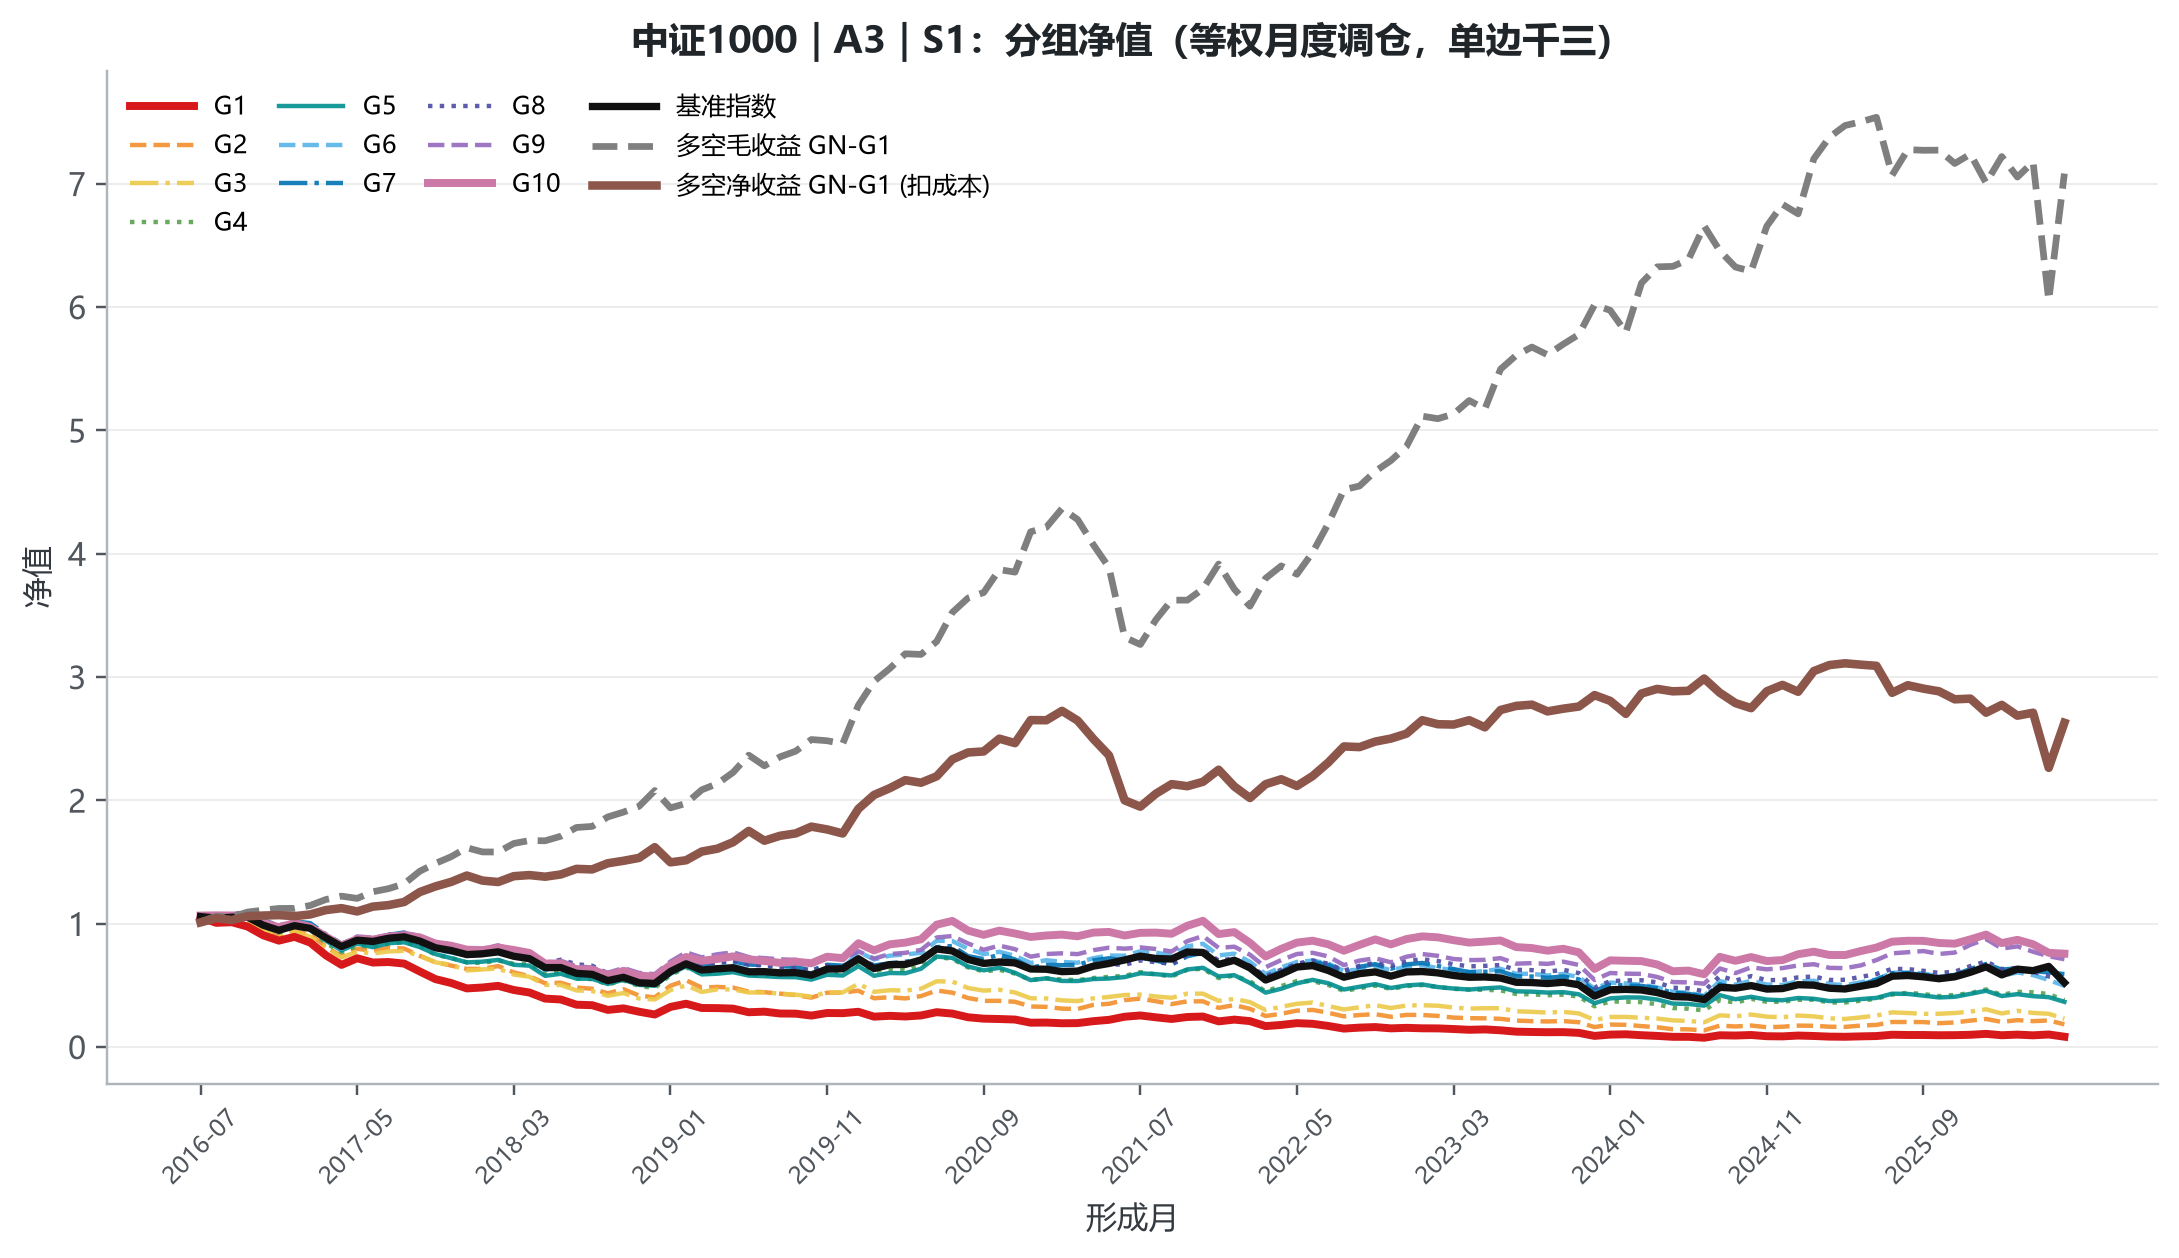
\includegraphics[width=.95\textwidth]{figs_v21/fig_2_1_zz1000_A3_group_nav.png}
\caption*{\textbf{\textcolor{reportred}{图 2-1}}　中证1000 / A3 / S1：分组净值（等权月度调仓、单边千三）}
\end{figure}

\begin{quote}
注：十组净值近似严格单调（\(G_1\) 最差 → \(G_{10}\)
最优）；基准指数为黑色实线，毛多空以灰色虚线展示，扣成本后的净多空以棕色粗实线展示。毛/净双曲线将''信号''与''成本拖累''分离展示。
\end{quote}

\begin{itemize}
\tightlist
\item
  \textbf{时序稳定性与衰减}：分年 IC 全区间无完整负年份，但自 2017-2020
  年的 4\%\textasciitilde10\% 降至 2024 年 3.6\%、2025 年 2.0\%、2026
  上半年约
  0------与行业观察同频的微观结构漂移（量化资金占比、程序化交易结构变化）。
\end{itemize}

\begin{longtable}[]{@{}
  >{\raggedright\arraybackslash}p{(\linewidth - 22\tabcolsep) * \real{0.0833}}
  >{\raggedright\arraybackslash}p{(\linewidth - 22\tabcolsep) * \real{0.0833}}
  >{\raggedright\arraybackslash}p{(\linewidth - 22\tabcolsep) * \real{0.0833}}
  >{\raggedright\arraybackslash}p{(\linewidth - 22\tabcolsep) * \real{0.0833}}
  >{\raggedright\arraybackslash}p{(\linewidth - 22\tabcolsep) * \real{0.0833}}
  >{\raggedright\arraybackslash}p{(\linewidth - 22\tabcolsep) * \real{0.0833}}
  >{\raggedright\arraybackslash}p{(\linewidth - 22\tabcolsep) * \real{0.0833}}
  >{\raggedright\arraybackslash}p{(\linewidth - 22\tabcolsep) * \real{0.0833}}
  >{\raggedright\arraybackslash}p{(\linewidth - 22\tabcolsep) * \real{0.0833}}
  >{\raggedright\arraybackslash}p{(\linewidth - 22\tabcolsep) * \real{0.0833}}
  >{\raggedright\arraybackslash}p{(\linewidth - 22\tabcolsep) * \real{0.0833}}
  >{\raggedright\arraybackslash}p{(\linewidth - 22\tabcolsep) * \real{0.0833}}@{}}
\caption{表 5　A3 分年 IC（中证1000，S1）}\tabularnewline
\toprule\noalign{}
\begin{minipage}[b]{\linewidth}\raggedright
年
\end{minipage} & \begin{minipage}[b]{\linewidth}\raggedright
2016H2
\end{minipage} & \begin{minipage}[b]{\linewidth}\raggedright
2017
\end{minipage} & \begin{minipage}[b]{\linewidth}\raggedright
2018
\end{minipage} & \begin{minipage}[b]{\linewidth}\raggedright
2019
\end{minipage} & \begin{minipage}[b]{\linewidth}\raggedright
2020
\end{minipage} & \begin{minipage}[b]{\linewidth}\raggedright
2021
\end{minipage} & \begin{minipage}[b]{\linewidth}\raggedright
2022
\end{minipage} & \begin{minipage}[b]{\linewidth}\raggedright
2023
\end{minipage} & \begin{minipage}[b]{\linewidth}\raggedright
2024
\end{minipage} & \begin{minipage}[b]{\linewidth}\raggedright
2025
\end{minipage} & \begin{minipage}[b]{\linewidth}\raggedright
2026H1
\end{minipage} \\
\midrule\noalign{}
\endfirsthead
\toprule\noalign{}
\begin{minipage}[b]{\linewidth}\raggedright
年
\end{minipage} & \begin{minipage}[b]{\linewidth}\raggedright
2016H2
\end{minipage} & \begin{minipage}[b]{\linewidth}\raggedright
2017
\end{minipage} & \begin{minipage}[b]{\linewidth}\raggedright
2018
\end{minipage} & \begin{minipage}[b]{\linewidth}\raggedright
2019
\end{minipage} & \begin{minipage}[b]{\linewidth}\raggedright
2020
\end{minipage} & \begin{minipage}[b]{\linewidth}\raggedright
2021
\end{minipage} & \begin{minipage}[b]{\linewidth}\raggedright
2022
\end{minipage} & \begin{minipage}[b]{\linewidth}\raggedright
2023
\end{minipage} & \begin{minipage}[b]{\linewidth}\raggedright
2024
\end{minipage} & \begin{minipage}[b]{\linewidth}\raggedright
2025
\end{minipage} & \begin{minipage}[b]{\linewidth}\raggedright
2026H1
\end{minipage} \\
\midrule\noalign{}
\endhead
\bottomrule\noalign{}
\endlastfoot
A3 分年 IC & 8.6\% & 10.1\% & 7.2\% & 4.3\% & 10.1\% & 3.3\% & 5.6\% &
6.4\% & 3.6\% & 2.0\% & 0.1\% \\
\end{longtable}

\begin{figure}[H]
\centering
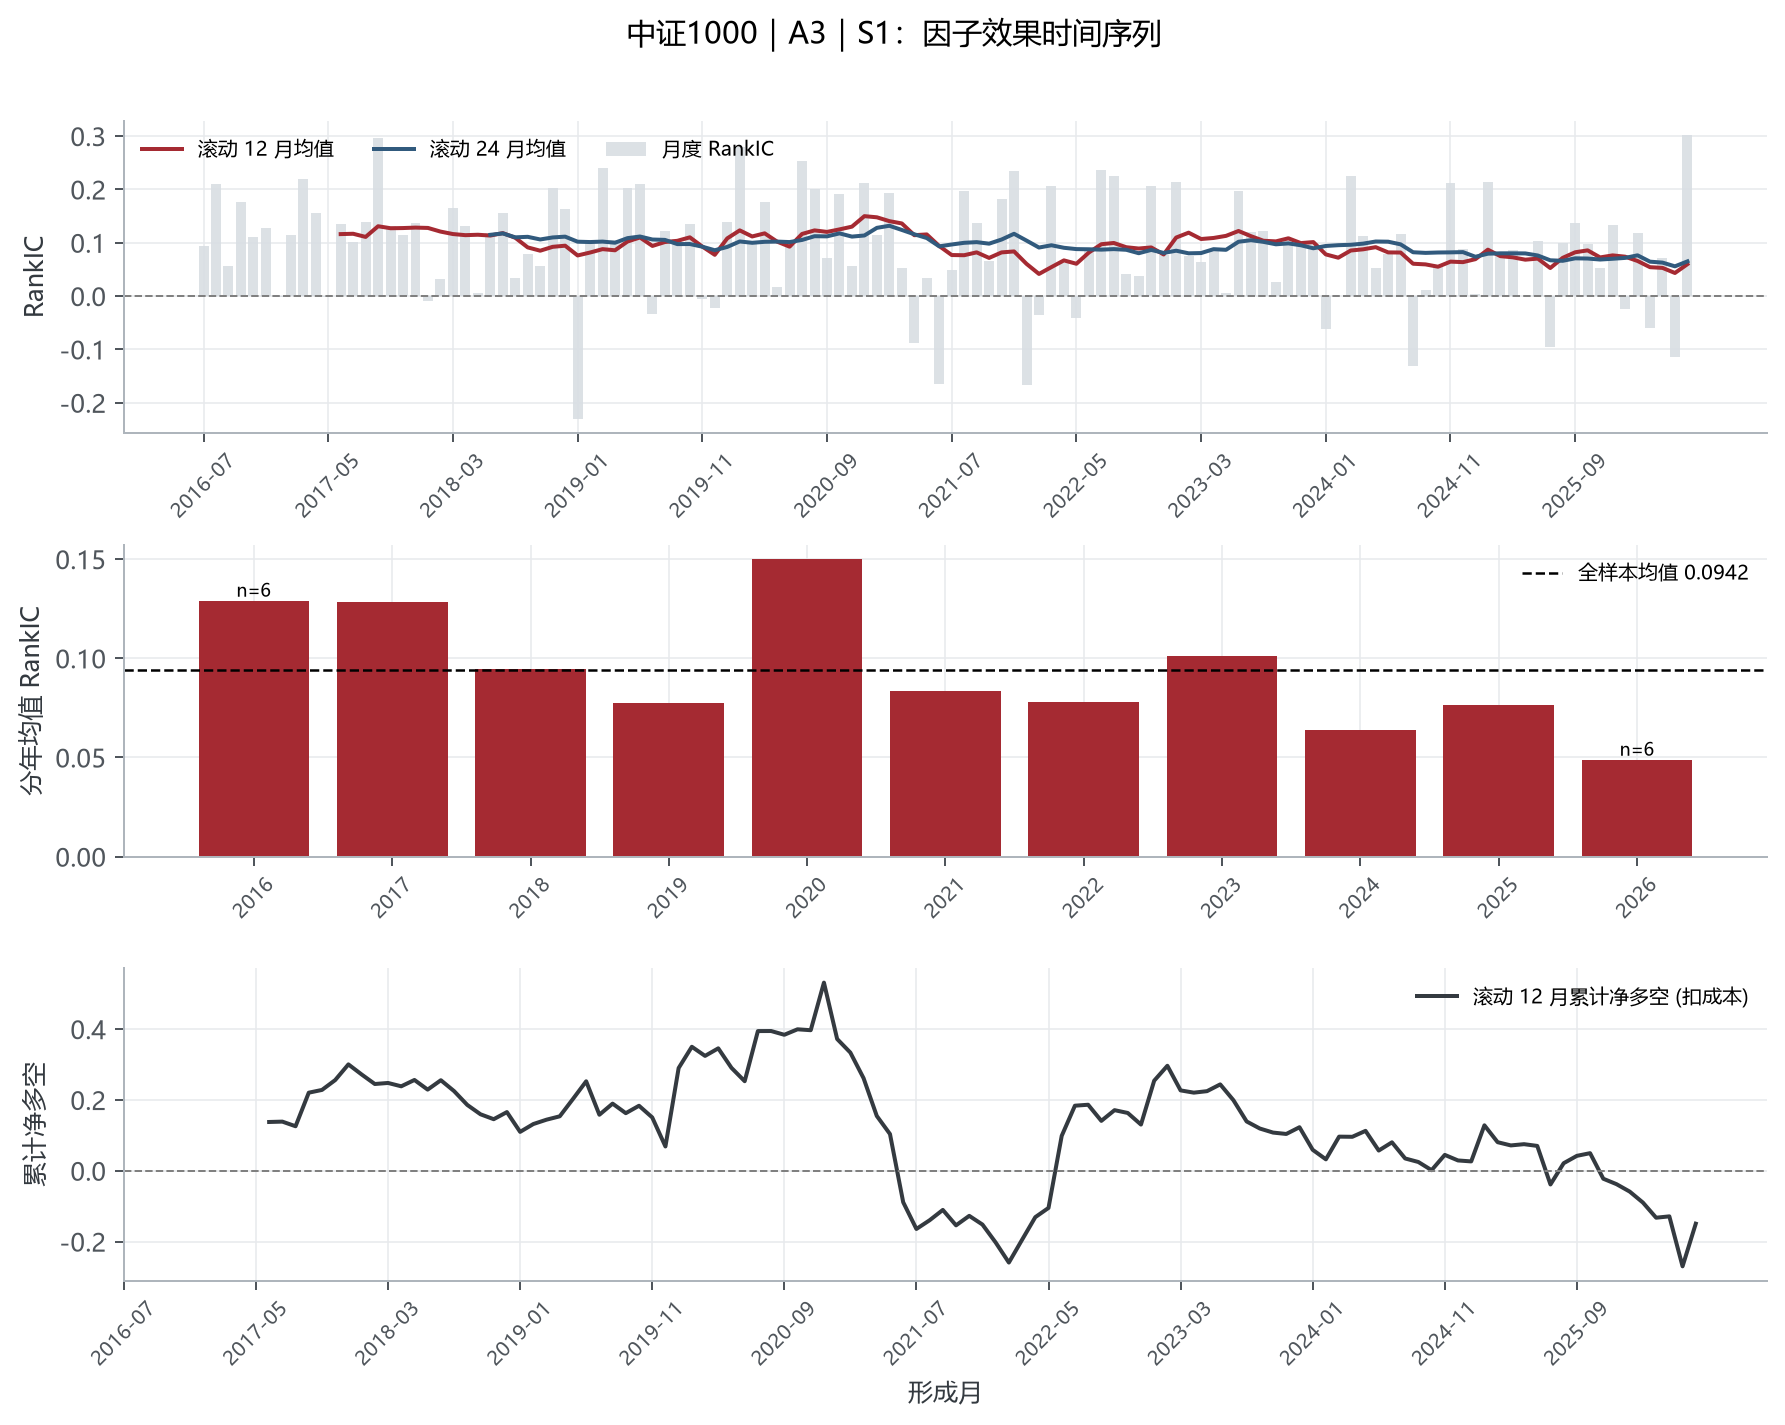
\includegraphics[width=.95\textwidth]{figs_v21/fig_2_2_zz1000_A3_decay.png}
\caption*{\textbf{\textcolor{reportred}{图 2-2}}　中证1000 / A3 / S1：因子效果时间序列衰减（上：月度 RankIC 与 12/24 月滚动；中：分年 RankIC；下：滚动 12 月净多空）}
\end{figure}

\begin{itemize}
\tightlist
\item
  \textbf{衰减度量确认（前后半 ICIR / 2025
  以来子样本；以下各因子同口径）}：中证1000/中证全指 S1 前半 ICIR
  3.68/3.84 → 后半 2.92/3.22，滚动 12 月 RankIC 年化趋势
  −0.6/−0.3pp；2025 年以来月均 RankIC 仍 +6.7\%/+8.0\%、方向胜率
  78\%/72\%------衰减存在但残差全体系最强，属''衰减而未失效''。
\end{itemize}

\begin{figure}[H]
\centering
\begin{minipage}[t]{0.49\textwidth}
\centering
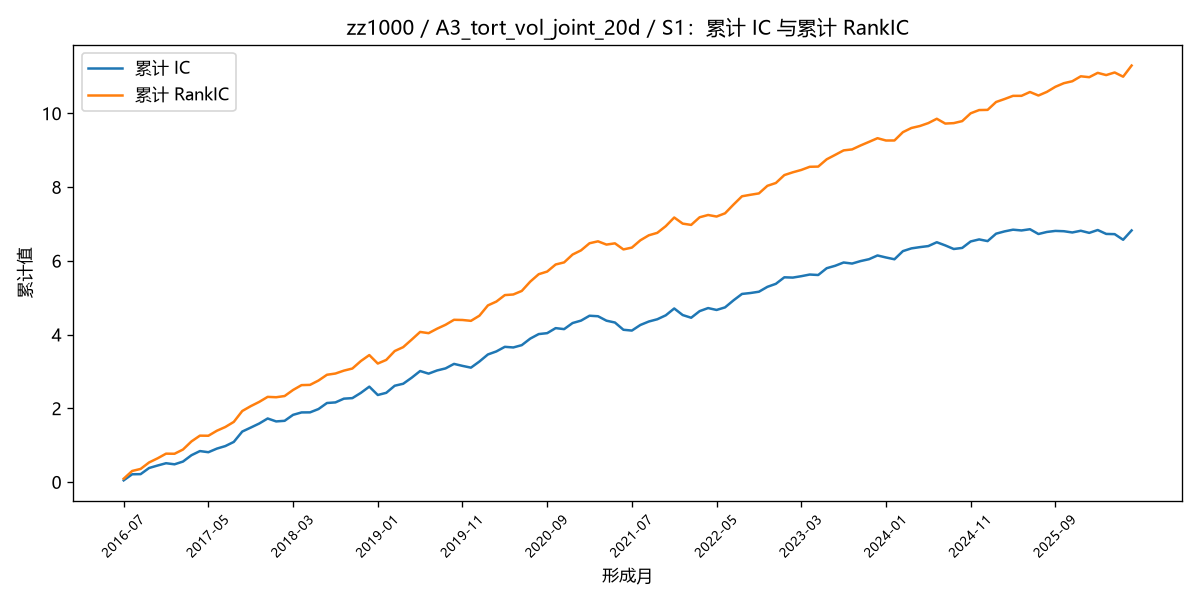
\includegraphics[width=\linewidth]{figs_v21/fig_2_3_zz1000_A3_cum_ic.png}
\vspace{2pt}\caption*{\textbf{\textcolor{reportred}{图 2-3}}　中证1000 / A3 / S1：累计 IC 与累计 RankIC}
\end{minipage}\hfill
\begin{minipage}[t]{0.49\textwidth}
\centering
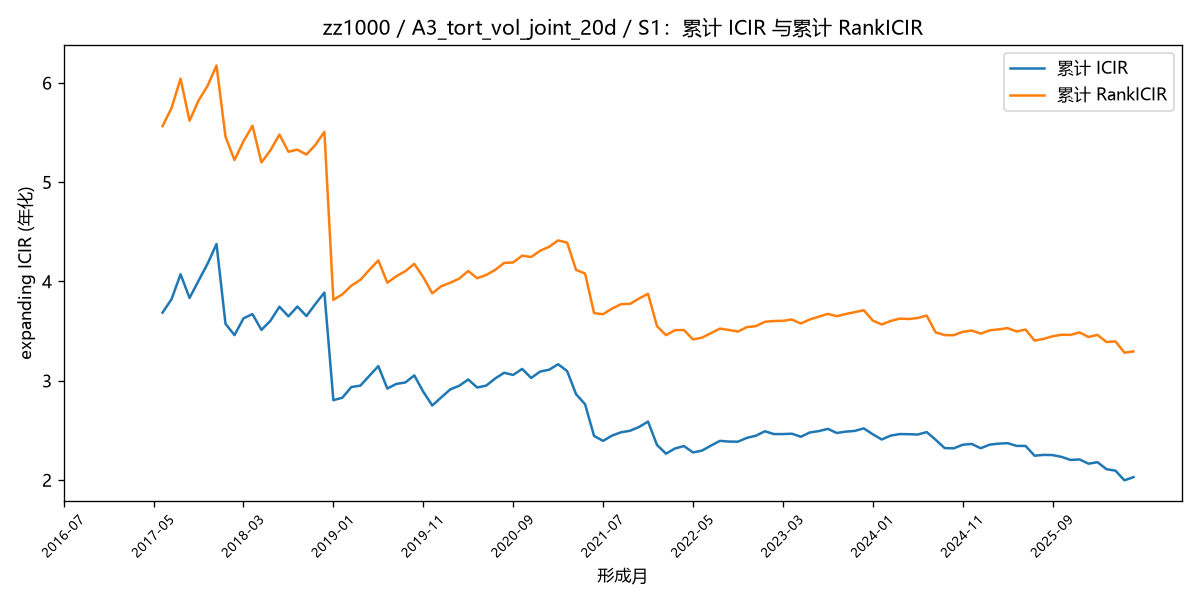
\includegraphics[width=\linewidth]{figs_v21/fig_2_4_zz1000_A3_cum_icir.png}
\vspace{2pt}\caption*{\textbf{\textcolor{reportred}{图 2-4}}　中证1000 / A3 / S1：累计 ICIR 与累计 RankICIR（expanding）}
\end{minipage}
\end{figure}

\textbf{③ A2c（高曲折成交集中度）：四池全显著的稳健型因子}

\begin{itemize}
\tightlist
\item
  与 A3 同源（均以高曲折时段为离散向量），但末端算子不同（成交占比 vs
  放量且逻辑）：中证1000 上 RankIC 8.52\% vs A3 的
  9.42\%，相关性高但不完全重合，可视作同一收益来源（噪音交易资金参与）的两种度量，\textbf{合成时宜取其一或等权}。分年
  IC 全部为正，2025 年降至 0.7\% 后 2026 上半年回升至 1.3\%。
\item
  \textbf{S1 与 S2 对照}：中证1000 3.13→1.56（−50\%）、中证全指
  3.36→1.86（−45\%）、沪深300 1.63→1.42（−13\%）------暴露结构同
  A3，但\textbf{大盘域衰减最小}，横截面稳定度略优于 A3。
\item
  \textbf{时序衰减}：前后半 ICIR 中证1000 3.33→2.92、中证全指
  3.50→3.20、沪深300 1.68→1.59，各池仅轻度衰减；2025 年以来月均 RankIC
  +5.8\%/+7.8\%（中证1000/中证全指，方向胜率均 78\%），为模块 A
  时序最稳者。
\end{itemize}

\begin{figure}[H]
\centering
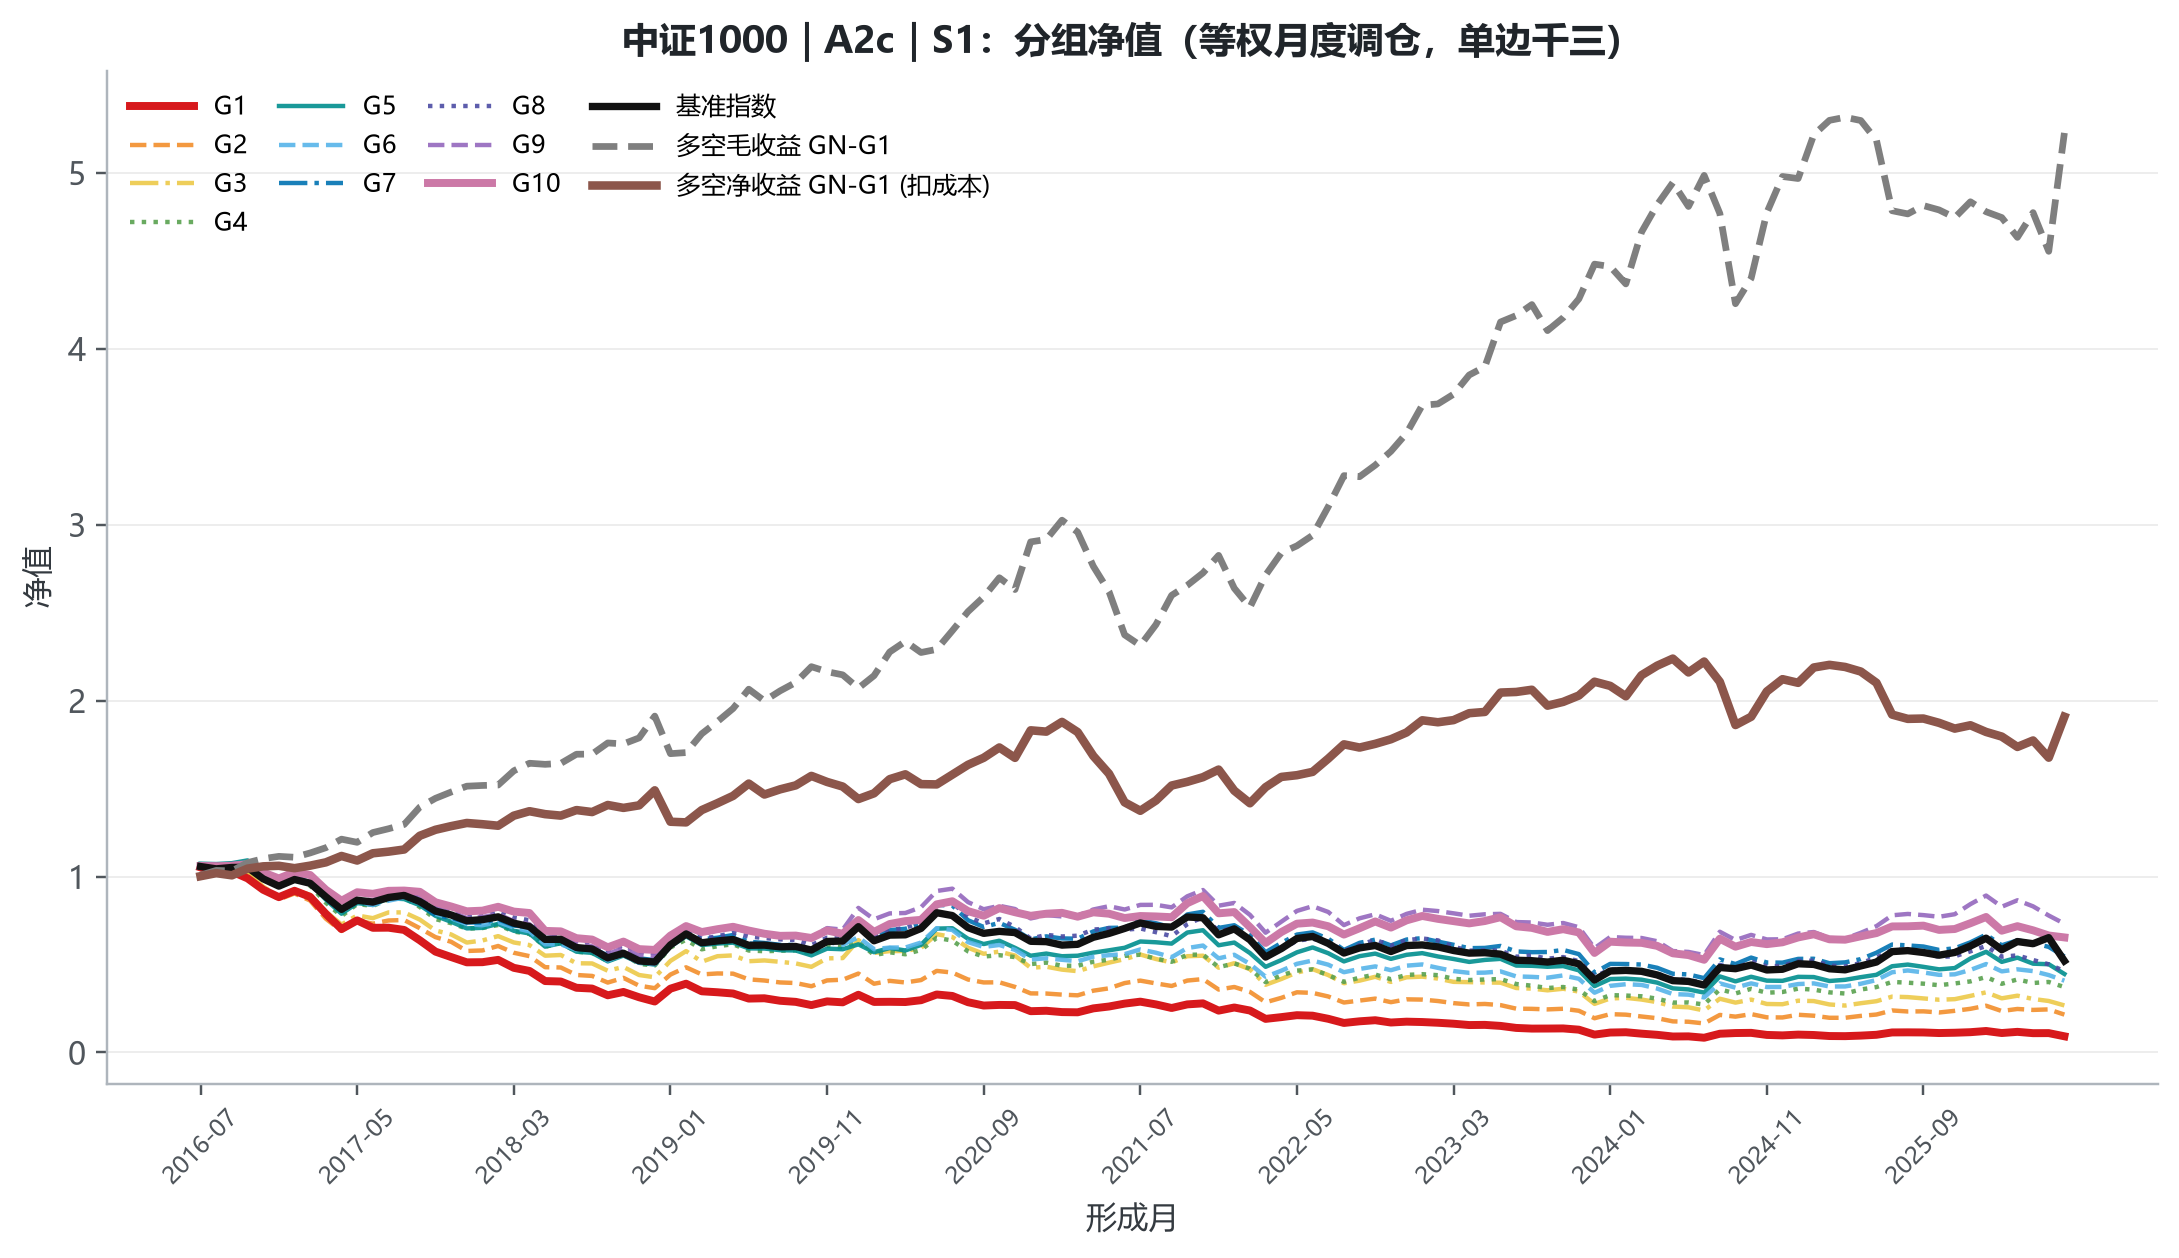
\includegraphics[width=.95\textwidth]{figs_v21/fig_2_5_zz1000_A2c_group_nav.png}
\caption*{\textbf{\textcolor{reportred}{图 2-5}}　中证1000 / A2c / S1：分组净值（$G\_1$ −21.4\% → $G\_\{10\}$ −4.5\%，毛多空 +18.0\%、有效净多空 +6.67\%）}
\end{figure}

\textbf{④ A2b（低曲折信息驱动收益）：小盘域显著的反转来源}

\begin{itemize}
\tightlist
\item
  中证1000/中证全指 S1 RankICIR
  −2.22/−1.99，即''低曲折时段累计收益高''者未来跑输------低曲折时段的''平滑推进''在月度频率上呈现\textbf{反转}而非动量，说明\textbf{以曲折度切割分离的收益逻辑更接近反转来源}。
\item
  \textbf{S1 与 S2 对照}：中证1000 −2.22→−1.09、中证全指
  −1.99→−0.93（衰减约
  50\%），方向在小盘域仍保持负向但显著性下降------反转来源部分与量价风格重合。
\item
  \textbf{时序衰减}：前后半 ICIR 中证1000 −2.45/−1.97、中证全指
  −2.03/−1.93，幅度稳定、无实质衰减；2025 年以来月均 RankIC
  −3.9\%/−4.0\%（方向胜率 78\%/72\%），反转来源近期仍有效。
\end{itemize}

\textbf{⑤ A2d（高曲折换手强度）：负向信息几乎全部借自换手暴露}

\begin{itemize}
\tightlist
\item
  中证1000/中证全指 S1 RankICIR −2.59/−2.82，负向显著；但 \textbf{S2
  后方向翻转}为 +0.62/+0.54（沪深300 亦由 −0.70 翻为
  +1.29）------负向来源几乎完全''借自''换手率暴露（高换手组本就跑输），剥离后信号消失。其''高换手×高曲折''的可交易方向（\(G_1-G_N\)）净收益可观（见
  5.5 节），本质是低换手异象的另一种表达。
\item
  \textbf{时序衰减}：负向来源在时序上并未衰减------中证全指后半 ICIR
  幅度反而扩大（−2.52→−3.11）、中证1000 −2.60→−2.56 稳定；2025
  年以来月均 RankIC −6.3\%/−8.9\%（方向胜率均
  72\%）。衰减的是其''独立性''（S2 后翻转），而非时序强度。
\end{itemize}

\textbf{⑥ A1/A1v（总量层）与 A2a（噪音强度）：基本无效}

\begin{itemize}
\tightlist
\item
  \textbf{A1}：S1 全池 RankICIR 仅 0.24\textasciitilde0.95，且 S2
  后暴露不稳定（中证全指 0.95→1.32 反而升、沪深300
  0.24→0.12）------``当日整体噪音大小''不携带稳定的月度选股信息；量加权变体
  \textbf{A1v} 更弱（S1 全池 \textbar RankICIR\textbar{} ≤ 0.26，S2
  后亦无改善）。
\item
  \textbf{A2a}：S1 中证全指 −1.58，\textbf{S2 后翻转为
  +0.50}------纯价格噪音强度与量价风格高度缠绕，无独立增量。
\item
  \textbf{时序衰减}：A1 后半 ICIR 各池衰减趋零（中证1000
  0.74→0.04），本已偏弱、时序上进一步走弱；A1v 方向跨池漂移（中证1000
  +0.23→−0.82），无衰减结论；A2a 则负向增强（沪深300
  −0.05→−1.15、中证全指 −1.30→−1.84），2025 年以来月均 RankIC
  −4.4\%/−4.6\%（方向胜率
  67\%/72\%）------近期噪音强度信息增强，与高波来源同向。
\end{itemize}

\textbf{⑦ 模块小结}

结构优于总量的判断成立------从 A1（0.24\textasciitilde0.95）到
A2c/A3（1.6\textasciitilde3.5）的跃升说明，只有当时间段切割能够分离经济含义相反的状态时才会产生增量；但需诚实标注，A3/A2c
的强信号约有一半借自波动率/换手率暴露（S1→S2 约打对折），模块 A
在组合中应作为''暴露管理型''因子使用；A2b/A2d
的负向信号则分别指向反转与低换手来源。

\begin{center}\rule{0.5\linewidth}{0.5pt}\end{center}

\section{三、模块
B：时序特征类因子------量价交互的方向性}\label{ux4e09ux6a21ux5757-bux65f6ux5e8fux7279ux5f81ux7c7bux56e0ux5b50ux91cfux4ef7ux4ea4ux4e92ux7684ux65b9ux5411ux6027}

\subsection{3.1 构建动机}\label{ux6784ux5efaux52a8ux673a-1}

模块 B
旨在刻画\textbf{量价交互的''方向性''信息------谁先动、哪边重、趋势有无交易确认}。量价相关性（同期相关）仅回答''量与价同向还是反向''，\textbf{不区分先后}；而微观结构上，``量领先价''（先放量后动价）与''价领先量''（先动价后放量）携带相反的博弈含义。模块
B 沿''\textbf{先后 × 上下 × 条件 × 背离}''四个方向展开：

\begin{enumerate}
\def\labelenumi{\arabic{enumi}.}
\tightlist
\item
  \textbf{先后（B1）}：多阶滞后交叉相关，识别信息是先经成交量泄露（知情建仓）还是先由价格带动（情绪追涨）；
\item
  \textbf{上下（B2/B2a）}：上行分钟与下行分钟量加权振幅之比，刻画多空力量对比；
\item
  \textbf{条件化（B3/B4）}：分涨跌考察先后（吸筹/出货结构），以及力量与信息的交互项；
\item
  \textbf{趋势确认与背离（B5a/B5b/B5c）}：量价确认度是否在日内衰减、两条累计路径斜率是否相反、创新高时量能是否不足------背离为低频经典维度，与高频''先后''正交。
\end{enumerate}

\subsection{3.2
因子定义与计算方法}\label{ux56e0ux5b50ux5b9aux4e49ux4e0eux8ba1ux7b97ux65b9ux6cd5-1}

统一记号同模块 A；另设分钟量变化率
\(\Delta v_t=(V_t-V_{t-1})/V_{t-1}\)（前量 \(\le0\) 处无定义）、量差分
\(\Delta V_t=V_t-V_{t-1}\)、日内累计价格路径
\(P_t=\sum_{s\le t}r_s\)、累计量偏离路径
\(Q_t=\sum_{s\le t}(V_s-\bar V)\)。以下同样按''数据变换 → K
线聚合''算子链逐因子给出，因子末端必为 20 日滚动均值。

\textbf{B1 量价领先滞后因子}

\begin{enumerate}
\def\labelenumi{\arabic{enumi}.}
\tightlist
\item
  \textbf{数据变换}（滞后·除法）：分钟量变化率 \(\Delta v_t\)；
\item
  \textbf{K 线聚合}（滞后交叉相关）：量领先价
  \(\rho_{+k}=\mathrm{Corr}(\Delta v_{t-k},r_t)\)、价领先量
  \(\rho_{-k}=\mathrm{Corr}(r_{t-k},\Delta v_t)\)（\(k=1,2,3\)，有效样本对
  \(<20\) 的阶剔除）；
\item
  \textbf{数据变换}（减法）：各阶领先滞后差 \(\rho_{+k}-\rho_{-k}\)；
\item
  \textbf{数据变换}（加权平均）：按 \(1/k\) 信息衰减加权
  \(LL=\dfrac{\sum_{k=1}^{3}\frac{1}{k}(\rho_{+k}-\rho_{-k})}{\sum_{k=1}^{3}\frac{1}{k}}\)；
\item
  \textbf{K 线聚合}（20 日均值）：\(F_{B1}=\mathrm{Mean}_{20d}(LL)\)。
\end{enumerate}

\textbf{B2 上行路径量能不对称因子}

\begin{enumerate}
\def\labelenumi{\arabic{enumi}.}
\tightlist
\item
  \textbf{数据变换}（0-1 化）：上行/下行标记
  \(d_t^+=\mathbb{1}\{r_t>0\}\)、\(d_t^-=\mathbb{1}\{r_t<0\}\)；
\item
  \textbf{数据变换}（乘法）：振幅 × 成交量 \(a_tV_t\)；
\item
  \textbf{K
  线聚合}（加权求和）：\(A^+=\sum_{d_t^+=1}a_tV_t\)、\(A^-=\sum_{d_t^-=1}a_tV_t\)；
\item
  \textbf{数据变换}（除法）：\(PA=\dfrac{A^+}{A^-+\varepsilon}\)；
\item
  \textbf{K 线聚合}（20 日均值）：\(F_{B2}=\mathrm{Mean}_{20d}(PA)\)。
\end{enumerate}

\textbf{B2a 上行路径成交额不对称因子}

\begin{enumerate}
\def\labelenumi{\arabic{enumi}.}
\tightlist
\item
  同 B2，仅第 2 步成交量列替换为成交额
  \(\mathrm{Amount}_t\)，其余算子链完全一致：\(F_{B2a}=\mathrm{Mean}_{20d}(PA_{\mathrm{amt}})\)。
\end{enumerate}

\textbf{B3 方向条件化量价领先滞后因子}

\begin{enumerate}
\def\labelenumi{\arabic{enumi}.}
\tightlist
\item
  \textbf{数据变换}（0-1 化）：按 \(r_t\)
  符号划分上行子集（\(r_t>0\)）与下行子集（\(r_t<0\)）；
\item
  \textbf{K 线聚合}（条件相关）：上行子集领先滞后差
  \(LL^+=\mathrm{Corr}(\Delta v_{t-1},r_t\mid r_t>0)-\mathrm{Corr}(r_{t-1},\Delta v_t\mid r_t>0)\)，下行子集
  \(LL^-\) 同理（各子集样本 \(\ge15\)）；
\item
  \textbf{数据变换}（减法）：\(DLL=LL^+-LL^-\)；
\item
  \textbf{K 线聚合}（20 日均值）：\(F_{B3}=\mathrm{Mean}_{20d}(DLL)\)。
\end{enumerate}

\textbf{B4 量价力量动量交叉因子}

\begin{enumerate}
\def\labelenumi{\arabic{enumi}.}
\tightlist
\item
  \textbf{数据变换}（减法）：力量偏离 \(PA_d-1\)；
\item
  \textbf{数据变换}（乘法）：交互项 \(F_{B4,d}=(PA_d-1)\times LL_d\)；
\item
  \textbf{K 线聚合}（20
  日均值）：\(F_{B4}=\mathrm{Mean}_{20d}(F_{B4,d})\)。
\end{enumerate}

\textbf{B5a 日内量价确认度衰减因子}

\begin{enumerate}
\def\labelenumi{\arabic{enumi}.}
\tightlist
\item
  \textbf{K 线聚合}（滚动相关）：60 分钟窗口量价相关
  \(\rho_t=\mathrm{Corr}\big(r_s,\Delta V_s\big)_{s\in[t-59,t]}\)（过半有效即可）；
\item
  \textbf{数据变换}（减法）：早盘确认度
  \(\rho_{\mathrm{early}}=\rho_{59}\)（10:30）、收盘确认度
  \(\rho_{\mathrm{late}}=\rho_{239}\)，\(Decay=\rho_{\mathrm{late}}-\rho_{\mathrm{early}}\)；
\item
  \textbf{K 线聚合}（20
  日均值）：\(F_{B5a}=\mathrm{Mean}_{20d}(Decay)\)。
\end{enumerate}

\textbf{B5b 量价趋势斜率背离因子}

\begin{enumerate}
\def\labelenumi{\arabic{enumi}.}
\tightlist
\item
  \textbf{K 线聚合}（累计）：价格路径
  \(P_t=\sum_{s\le t}r_s\)、量偏离路径
  \(Q_t=\sum_{s\le t}(V_s-\bar V)\)；
\item
  \textbf{K
  线聚合}（回归斜率）：\(\hat\beta_p=\mathrm{Slope}(P_t,t)\)、\(\hat\beta_v=\mathrm{Slope}(Q_t,t)\)（有效点
  \(\ge20\)、无效占比 \(\le10\%\)）；
\item
  \textbf{数据变换}（标准化）：\(\hat\beta_p^s=\hat\beta_p/\mathrm{Std}(P_t)\)、\(\hat\beta_v^s=\hat\beta_v/\mathrm{Std}(Q_t)\)；
\item
  \textbf{数据变换}（乘法）：背离度
  \(Div=-\hat\beta_p^s\,\hat\beta_v^s\)；
\item
  \textbf{K 线聚合}（20 日均值）：\(F_{B5b}=\mathrm{Mean}_{20d}(Div)\)。
\end{enumerate}

\textbf{B5c 价格新高量能不足因子}

\begin{enumerate}
\def\labelenumi{\arabic{enumi}.}
\tightlist
\item
  \textbf{数据变换}（0-1 化）：新高标记
  \(h_t=\mathbb{1}\{P_t=\max_{s\le t}P_s\}\)；
\item
  \textbf{K 线聚合}（条件均值）：新高时平均量
  \(\mathrm{Mean}(V_t\mid h_t=1)\)、平时平均量
  \(\mathrm{Mean}(V_t\mid h_t=0)\)；
\item
  \textbf{数据变换}（除法）：\(VR=\dfrac{\mathrm{Mean}(V_t\mid h_t=1)}{\mathrm{Mean}(V_t\mid h_t=0)}\)；
\item
  \textbf{K 线聚合}（20 日均值）：\(F_{B5c}=\mathrm{Mean}_{20d}(VR)\)。
\end{enumerate}

\subsection{3.3
因子经济含义}\label{ux56e0ux5b50ux7ecfux6d4eux542bux4e49-1}

\begin{itemize}
\tightlist
\item
  \textbf{B1（量价领先滞后）}：\(\rho_{+k}\)
  占优（量领先价）表明信息先经成交量泄露再反映至价格------知情交易渐进建仓，具有短期动量延续性；\(\rho_{-k}\)
  占优（价领先量）表明价格先动、量能跟随------情绪追涨，具有短期反转特征。\(k=1,2,3\)
  按 \(1/k\) 信息衰减加权，有效样本对不足 20 的阶剔除。
\item
  \textbf{B2/B2a（路径不对称性）}：\(PA>1\)
  表明上行分钟量加权振幅更大，买方力量占优（吸筹/惜售），预期做多；以成交额替代成交量可消除低价股/小盘股的量级偏差。
\item
  \textbf{B3（条件化领先滞后）}：\(DLL=LL^+-LL^->0\)
  表明上行时量更领先价（知情买入）、下行时价更领先量（恐慌先行），为典型''吸筹''结构。
\item
  \textbf{B4（力量动量交叉）}：将''力量对比偏离
  1''与''信息模式方向''相乘，检验两种微观结构信号的\textbf{交互}是否携带独立信息。
\item
  \textbf{B5a（量价确认度衰减）}：日内量价同步性自早盘至收盘的变化，\(Decay<0\)
  表明趋势的交易确认在瓦解------\textbf{动量衰竭}的动态视角。
\item
  \textbf{B5b（趋势斜率背离）}：价格累计路径斜率与成交量累计偏离路径斜率方向相反（价涨量缩/价跌量增）→
  当前趋势缺乏交易确认，为背离的\textbf{静态对比}视角。
\item
  \textbf{B5c（新高量能不足）}：经典''顶背离''的量化版本，\(VR<1\)
  表明创新高时成交量低于平时------\textbf{追高缩量}，未来跑输。
\end{itemize}

\subsection{3.4
因子表现评估}\label{ux56e0ux5b50ux8868ux73b0ux8bc4ux4f30-1}

\textbf{① 因子总览（RankICIR；同因子 S1 一行、S2
一行，横向对比四股票池）}

\begin{longtable}{@{}p{3.0cm} c r r r r p{5.2cm}@{}}
\caption{表 6　模块 B 因子总览（RankICIR，S1/S2 四池）}\\
\toprule
因子 & 中性化 & 沪深300 & 中证500 & 中证1000 & 中证全指 & 判读 \\
\midrule
\endfirsthead
\toprule
因子 & 中性化 & 沪深300 & 中证500 & 中证1000 & 中证全指 & 判读 \\
\midrule
\endhead
\bottomrule
\endfoot
\multirow{2}{\hsize}{\textbf{B1 领先滞后}} & S1 & 0.62 & 0.85 & \textbf{1.34} & \textbf{1.44} & \multirow{2}{\hsize}{仅小盘域有效；S2 后全指衰减至 0.54} \\
 & S2 & 0.46 & 0.61 & 0.77 & 0.54 & \\
\cmidrule(lr){2-6}
\multirow{2}{\hsize}{\textbf{B2/B2a 不对称}} & S1 & −0.48 & −0.69 & −0.72 & −0.74 & \multirow{2}{\hsize}{全池弱负，S1/S2 均不显著} \\
 & S2 & −0.17 & −0.29 & −0.51 & −0.58 & \\
\cmidrule(lr){2-6}
\multirow{2}{\hsize}{\textbf{B3 条件化领先滞后}} & S1 & −0.75 & −0.90 & −0.77 & −0.88 & \multirow{2}{\hsize}{S2 后小盘/全指显著为负（−1.68/−2.03）} \\
 & S2 & −0.92 & −1.12 & −1.68 & −2.03 & \\
\cmidrule(lr){2-6}
\multirow{2}{\hsize}{\textbf{B4 力量动量交叉}} & S1 & −0.11 & −1.08 & −1.75 & \textbf{−3.09} & \multirow{2}{\hsize}{全指显著负向；S2 后 −2.10，经济含义需甄别} \\
 & S2 & −0.11 & −0.55 & −1.05 & −2.10 & \\
\cmidrule(lr){2-6}
\multirow{2}{\hsize}{\textbf{B5a 确认度衰减}} & S1 & −1.09 & −0.81 & −1.10 & \textbf{−1.35} & \multirow{2}{\hsize}{小盘/全指负向；S2 后约减半} \\
 & S2 & −0.98 & −0.44 & −0.52 & −0.87 & \\
\cmidrule(lr){2-6}
\multirow{2}{\hsize}{\textbf{B5b 斜率背离}} & S1 & 0.38 & 0.39 & 0.17 & 0.19 & \multirow{2}{\hsize}{S1/S2 均基本无效} \\
 & S2 & 0.43 & 0.46 & 0.23 & 0.23 & \\
\cmidrule(lr){2-6}
\multirow{2}{\hsize}{\textbf{B5c 新高量能不足}} & S1 & −1.90 & −2.06 & \textbf{−3.34} & \textbf{−3.71} & \multirow{2}{\hsize}{顶背离反转，四池全负向；S2 后仍显著（−1.74\textasciitilde{}−2.44）} \\
 & S2 & −1.82 & −0.87 & −1.85 & −2.44 & \\
\end{longtable}

\textbf{② B5c（价格新高量能不足）：模块 B 最强、时序最稳定的因子}

\begin{itemize}
\tightlist
\item
  \textbf{方向与稳定性}：RankIC 方向稳定为负------``创新高时缩量''者未来跑输，中证1000
  的 9 个完整年份 RankIC 均为负。按收益较高的低 \(VR\) 组做多、较低的高 \(VR\) 组做空后，
  分年净多空在 2017、2018、2020 和 2023 年分别为 +11.1\%、+15.0\%、+11.4\% 和 +11.0\%，
  但 2019、2021 和 2025 年为负，说明排序方向稳定不等于成本后多空收益逐年为正。经济含义上，
  该结果与高位成交确认不足和后续反转相符，但不能据此认定单一机制。
\item
  \textbf{S1 与 S2 对照}：中证1000 −3.34→−1.85（−45\%）、中证全指
  −3.71→−2.44（−34\%）、沪深300
  −1.90→−1.82（−4\%），量价中性后仍全部显著------负向来源在剥离波动/换手暴露后保持稳健，是模块
  B 中最接近独立维度的增量。
\end{itemize}

\begin{figure}[H]
\centering
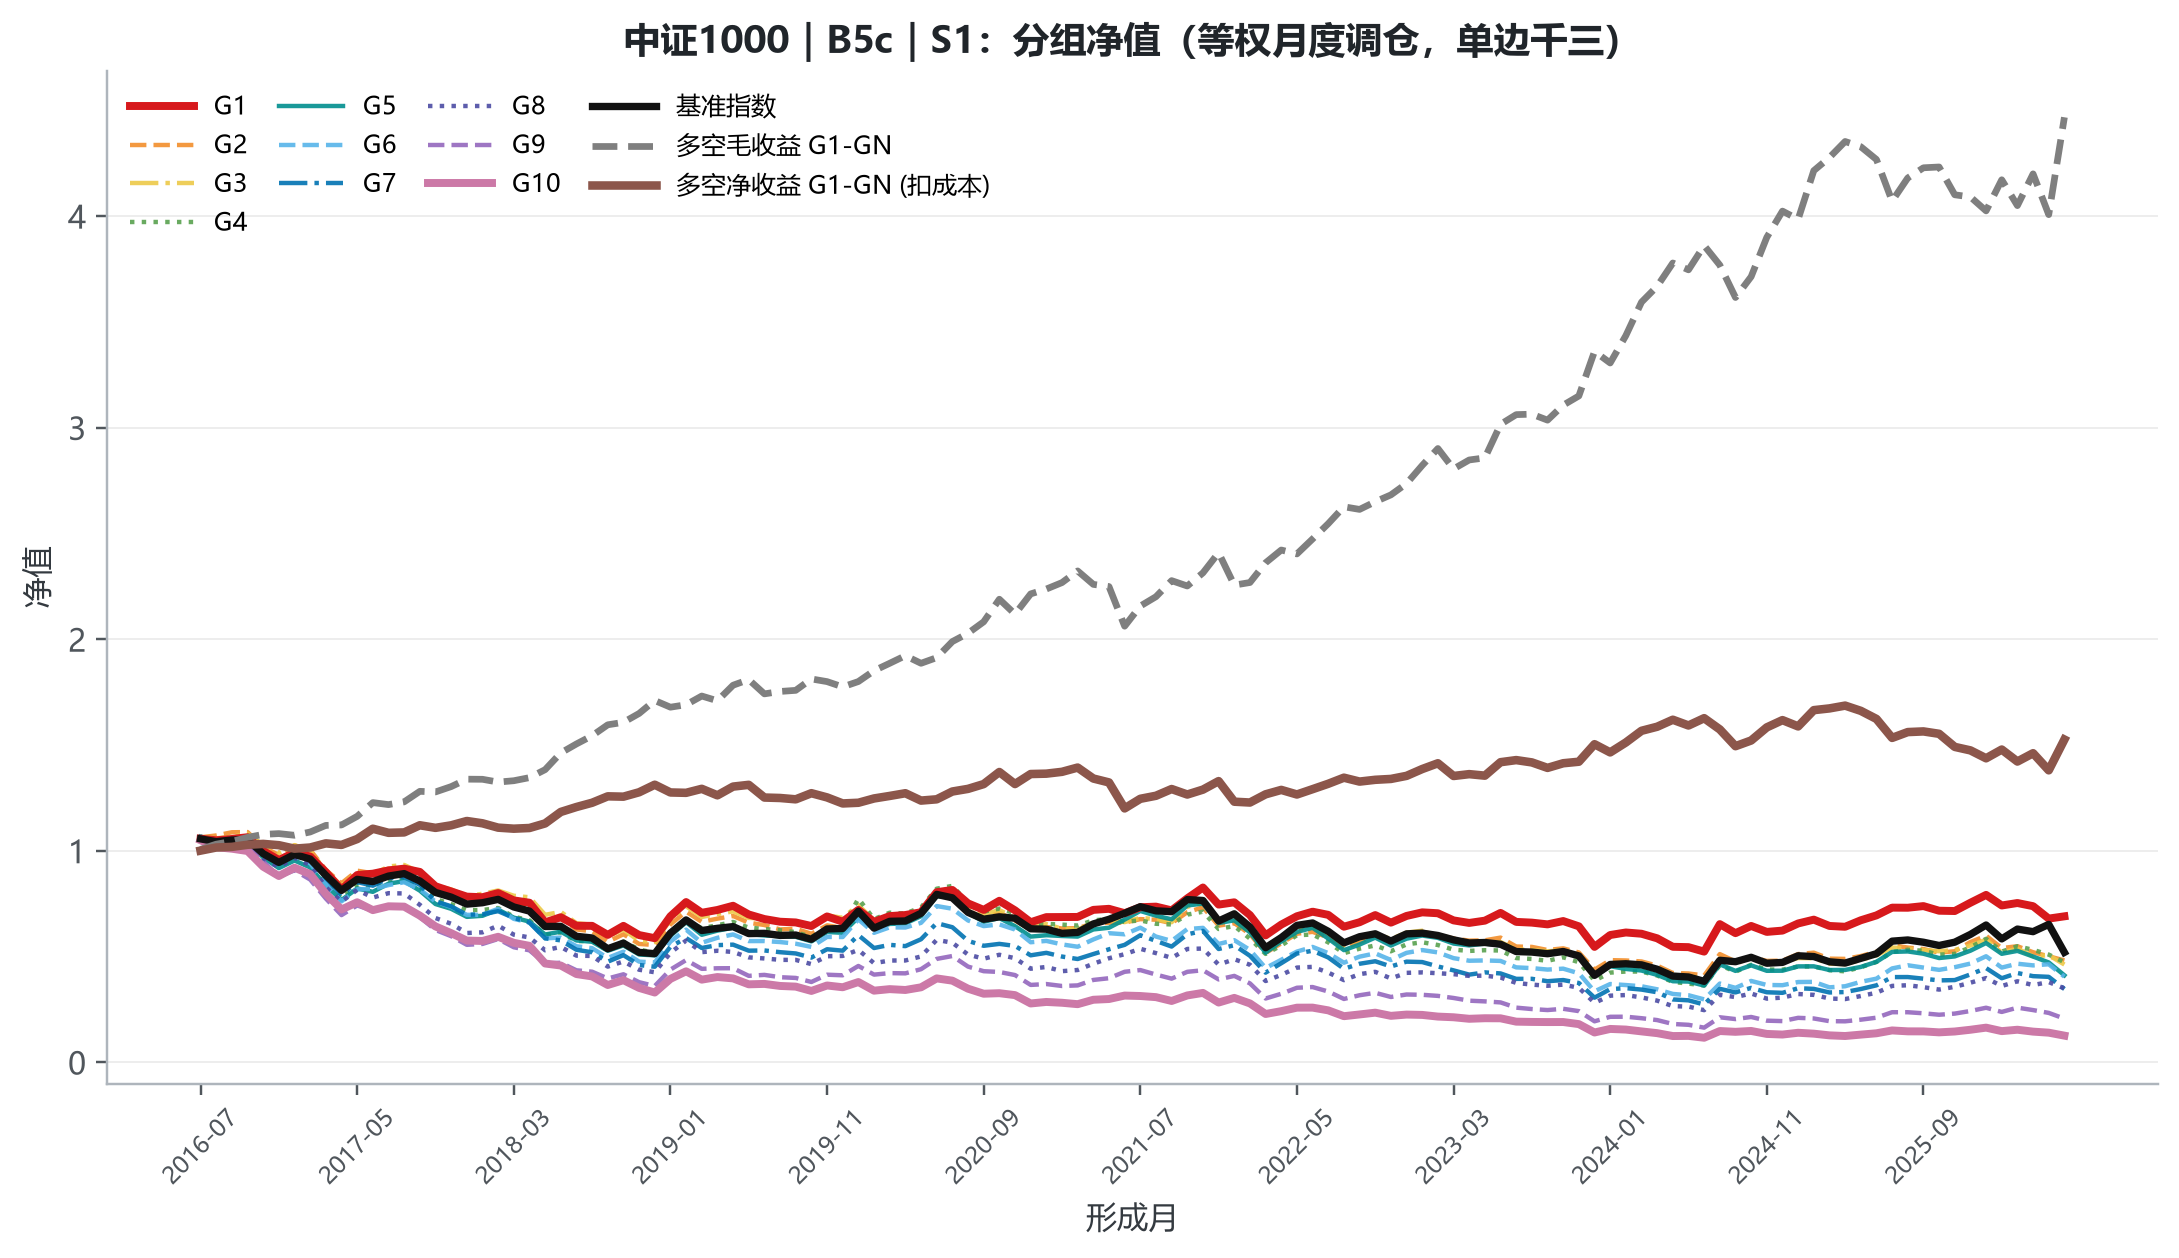
\includegraphics[width=.95\textwidth]{figs_v21/fig_3_1_zz1000_B5c_group_nav.png}
\caption*{\textbf{\textcolor{reportred}{图 3-1}}　中证1000 / B5c（价格新高量能不足）/ S1：分组净值（方向稳定为负，低 $VR$ 组持续跑赢高 $VR$ 组）}
\end{figure}

\begin{itemize}
\tightlist
\item
  \textbf{时序衰减}：前后半 ICIR 中证1000 −3.69→−3.03、中证全指
  −4.18→−3.34，幅度收缩约两成但各池仍高度显著；2025 年以来月均 RankIC
  −5.0\%/−6.0\%（方向胜率
  78\%/67\%）------顶背离来源时序最稳，近期未失效。
\end{itemize}

\begin{figure}[H]
\centering
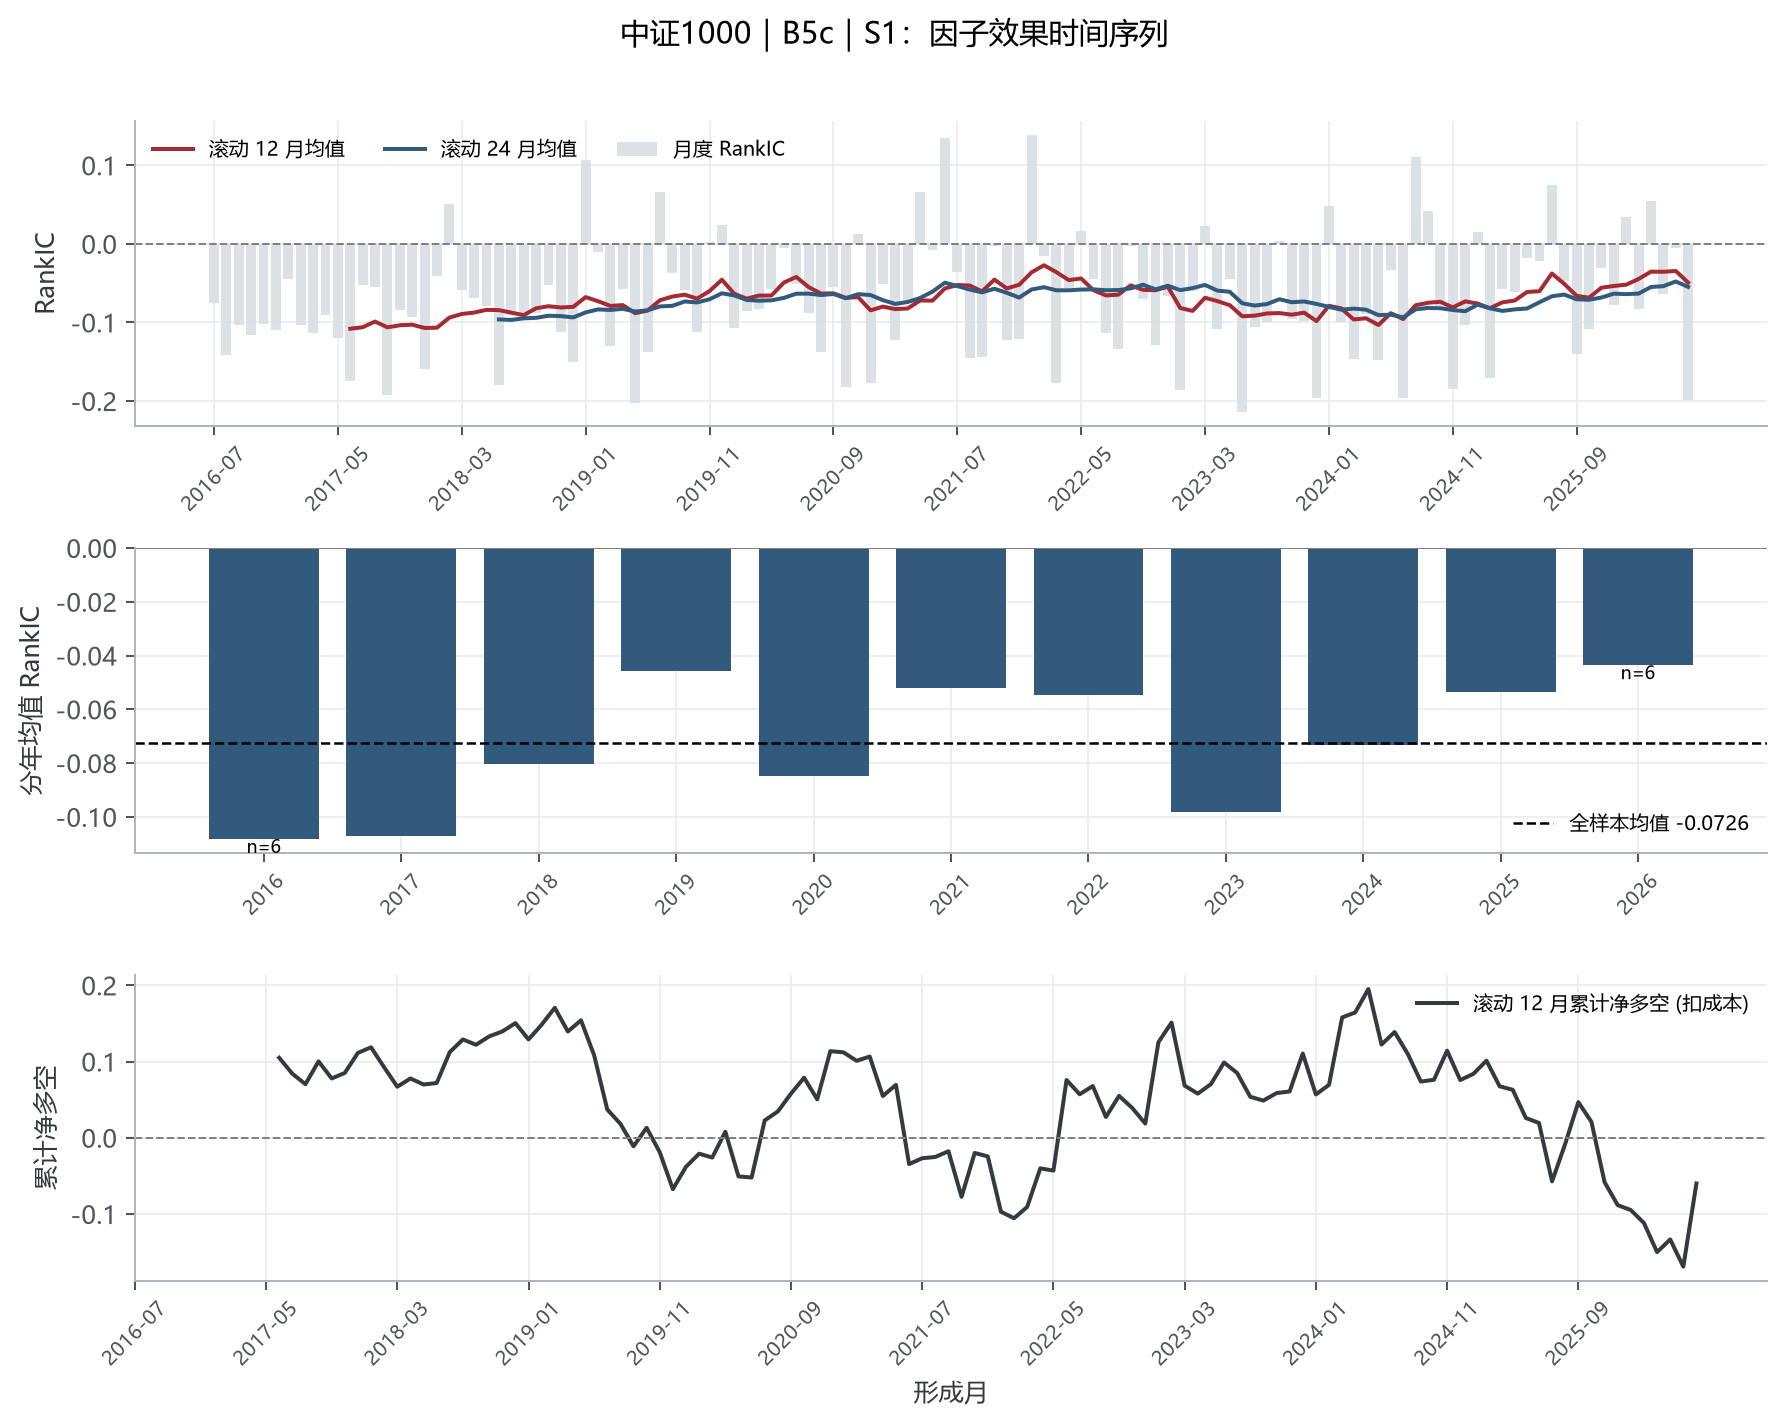
\includegraphics[width=.95\textwidth]{figs_v21/fig_3_2_zz1000_B5c_decay.png}
\caption*{\textbf{\textcolor{reportred}{图 3-2}}　中证1000 / B5c / S1：因子效果时间序列衰减（上：月度 RankIC 与 12/24 月滚动；中：分年 RankIC；下：滚动 12 月净多空）}
\end{figure}

\textbf{③ B1（量价领先滞后）：小盘域成立、大盘域失效}

\begin{itemize}
\tightlist
\item
  中证1000/中证全指 S1 RankICIR 1.34/1.44、毛多空约
  +9\textasciitilde10\%，``量领先价''者未来跑赢------信息渐进泄露（知情交易建仓）的叙事在小盘、高噪音域成立；沪深300
  衰减至 0.62。分年 IC 显示 2018-2024 多数年份在 1\% 上下徘徊、2025
  年回升至 3.0\%，信号持续性一般。
\item
  \textbf{S1 与 S2 对照}：中证1000 1.34→0.77、中证全指
  1.44→0.54（−63\%）、沪深300
  0.62→0.46------信息扩散叙事部分''借自''换手率来源，量价中性后显著性与稳定性均明显下降。
\item
  \textbf{时序衰减}：后半 ICIR 各池回落（中证全指 1.74→1.09、中证1000
  1.58→1.06），但 2025 年以来月均 RankIC +1.3\%/+1.4\%（方向胜率
  72\%/67\%），与分年 IC''2025 年回升至
  3.0\%``互相印证------领先滞后来源衰减而未消失，呈间歇性回归。
\end{itemize}

\begin{figure}[H]
\centering
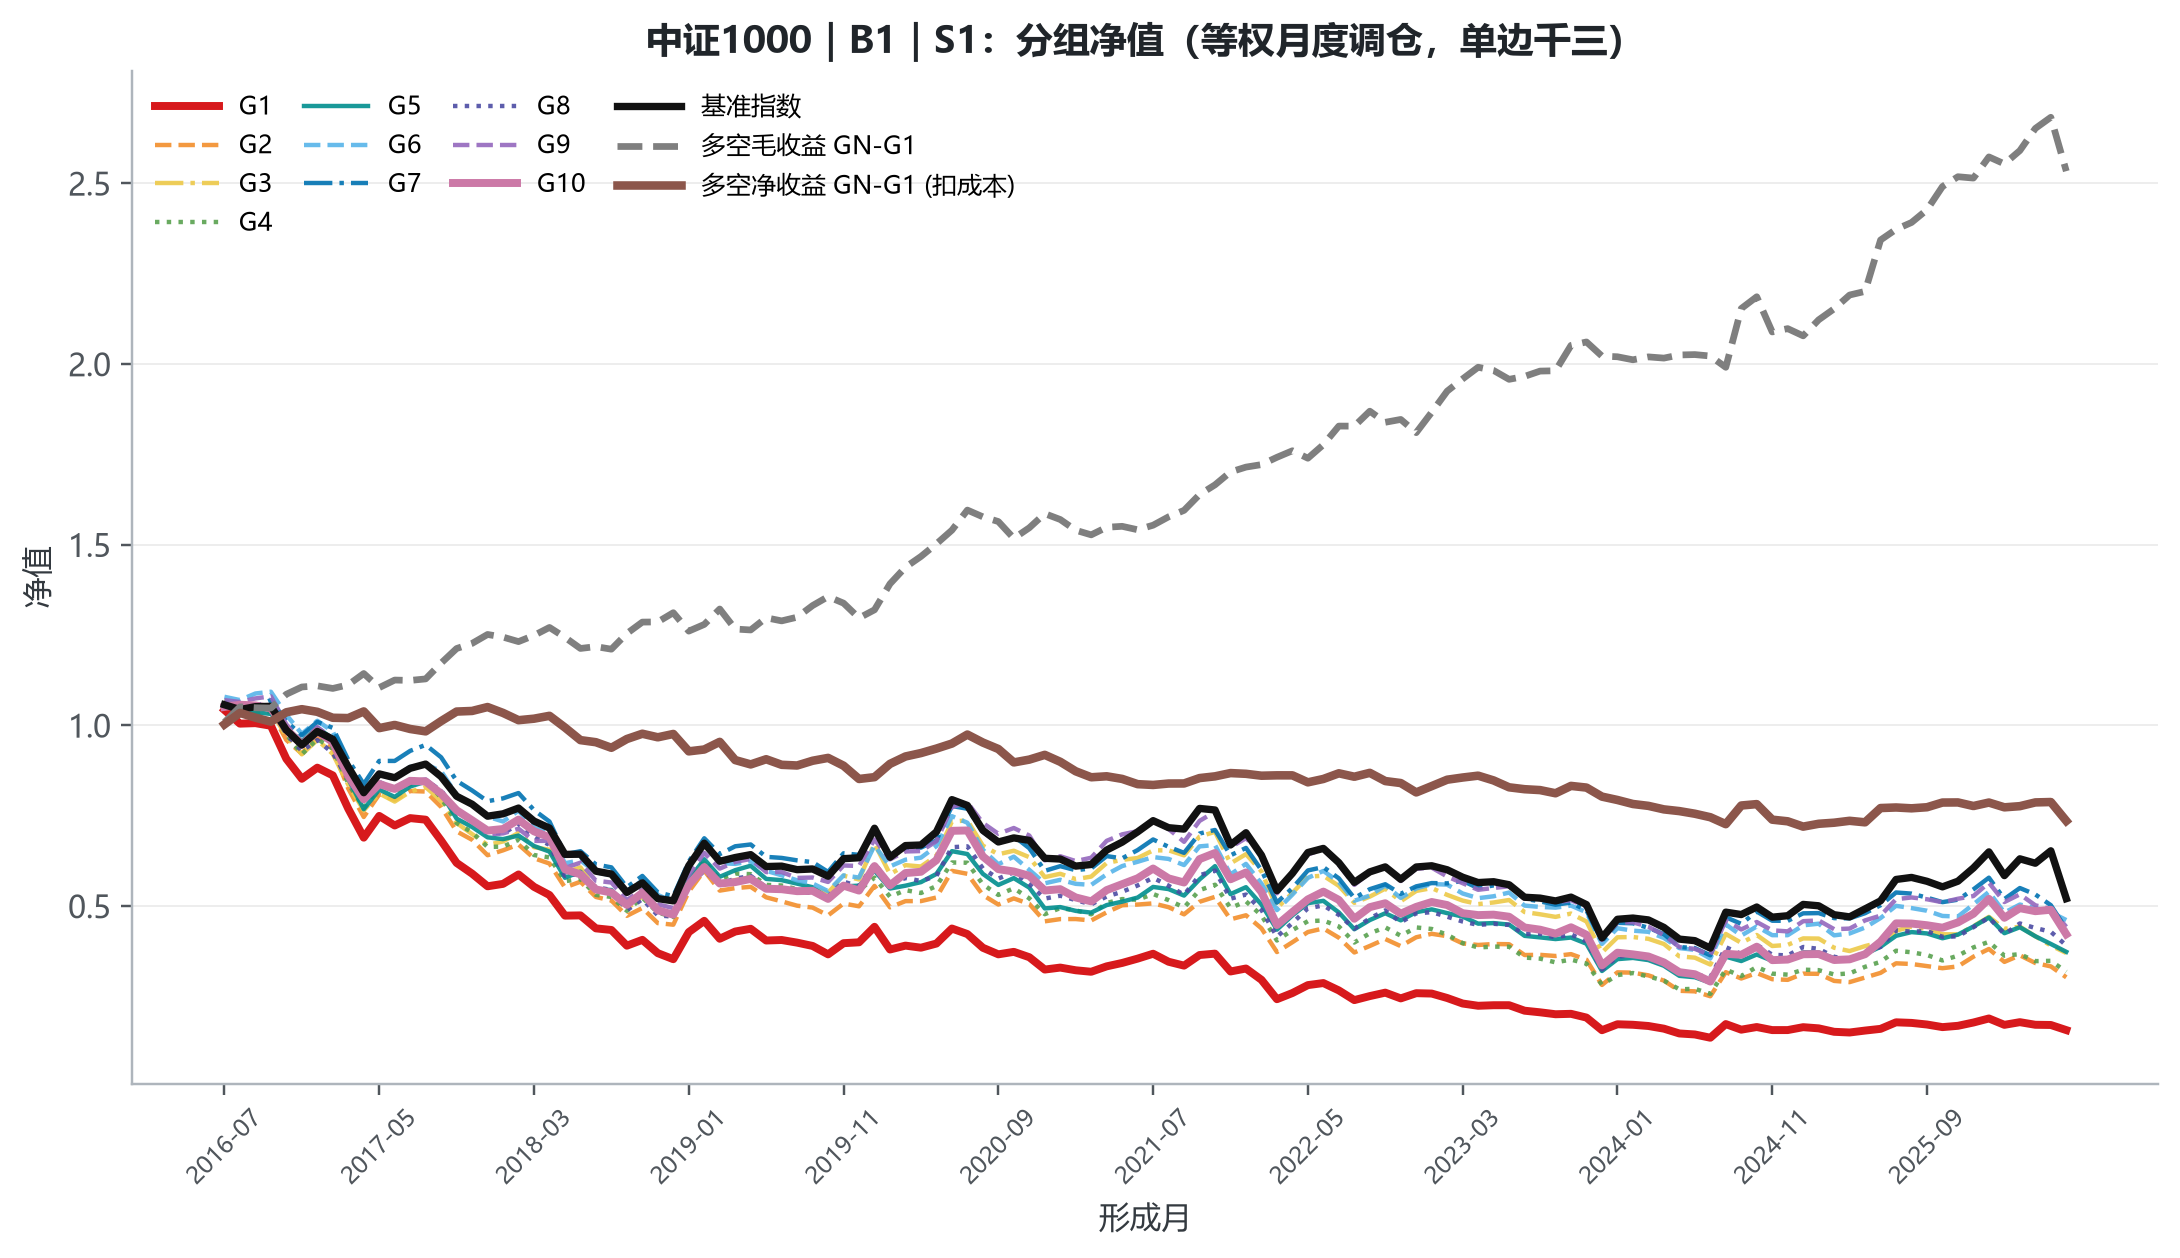
\includegraphics[width=.95\textwidth]{figs_v21/fig_3_3_zz1000_B1_group_nav.png}
\caption*{\textbf{\textcolor{reportred}{图 3-3}}　中证1000 / B1（量价领先滞后）/ S1：分组净值（$G\_1$ −17.2\% → $G\_\{10\}$ −8.6\%，毛多空 +9.7\%）}
\end{figure}

\textbf{④ B2/B2a（上下力量对比）：基本无效}

\begin{itemize}
\tightlist
\item
  全池 S1 RankICIR ≈ −0.7 不显著；\textbf{S2 后仍 ≈ −0.6
  不显著}（如中证全指 B2 −0.74→−0.58）------量价中性前后均无信号，``上行
  vs
  下行分钟哪边量更大''在月度频率上不构成可交易信息，这是对''路径不对称性''叙事的实证否定。
\item
  \textbf{时序衰减}：本就无效，前后半 ICIR 幅度均
  \textless1.1，无衰减问题；2025 年以来月均 RankIC 约
  −2\%\textasciitilde−4\%（方向胜率
  72\%）仅为负向弱残差，不改变''无效''判断。
\end{itemize}

\textbf{⑤ B3/B4（条件化与交互项）：S2 后增强但非独立增量}

\begin{itemize}
\tightlist
\item
  \textbf{B3}：S1 各池 ≈ −0.8 不显著，\textbf{S2 后中证1000/中证全指降至
  −1.68/−2.03（反而增强）}；\textbf{B4}：S1 中证全指 −3.09、S2 后
  −2.10，同样保持显著。然而条件化与交互项由 B1/B2
  派生、经济含义模糊，在量价中性化检验下难以构成\textbf{独立}来源，更接近对已知来源的重新打包，暂不建议单独入库。
\item
  \textbf{时序衰减}：二者为全体系衰减最重者------B4 中证全指前半 ICIR
  −4.10 → 后半 −2.29、中证500 −1.82→−0.29；B3
  沪深300/中证全指后半幅度收缩至近零（−1.61→−0.10/−0.07）；2025
  年以来月均 RankIC：B4 中证全指 −1.8\%（方向胜率
  72\%，但幅度不足前半之半）、B3 各池在 ±1\% 以内且原负向方向胜率仅
  56\%\textasciitilde61\%------条件化领先滞后与交互项的 alpha 在 2023
  年后基本消失，``S2 后增强''更多是前半借自来源的残差展示。
\end{itemize}

\textbf{⑥ B5a/B5b（确认度衰减 vs 斜率背离）：动态视角胜出}

\begin{itemize}
\tightlist
\item
  \textbf{B5a}：中证1000/中证全指 S1 RankICIR −1.10/−1.35
  显著为负（量价确认度衰减→未来跑输），\textbf{S2 后降至
  −0.52/−0.87（衰减约
  50\%）}------动态衰减视角部分借自量价暴露，且方向在 2023
  年后转正、近期衰减。
\item
  \textbf{B5b}：全池 S1 RankICIR 仅 0.17\textasciitilde0.39，\textbf{S2
  后几乎不变（中证全指
  0.19→0.23）}，始终无效------``两条累计路径斜率相反''的静态对比不构成信号。动态视角（相关性在日内衰减）优于静态对比（斜率方向相反）。
\item
  \textbf{时序衰减}：B5a 是典型的''消失''案例------中证1000/中证全指前半
  ICIR −2.41/−2.91 → 后半 −0.10/−0.21，2025 年以来月均 RankIC
  反为弱正（+1.3\%/+2.0\%），与全样本负向方向相反：确认度衰减来源约在
  2023 年后被市场消化；B5b 本就无效，无衰减问题。
\end{itemize}

\begin{figure}[H]
\centering
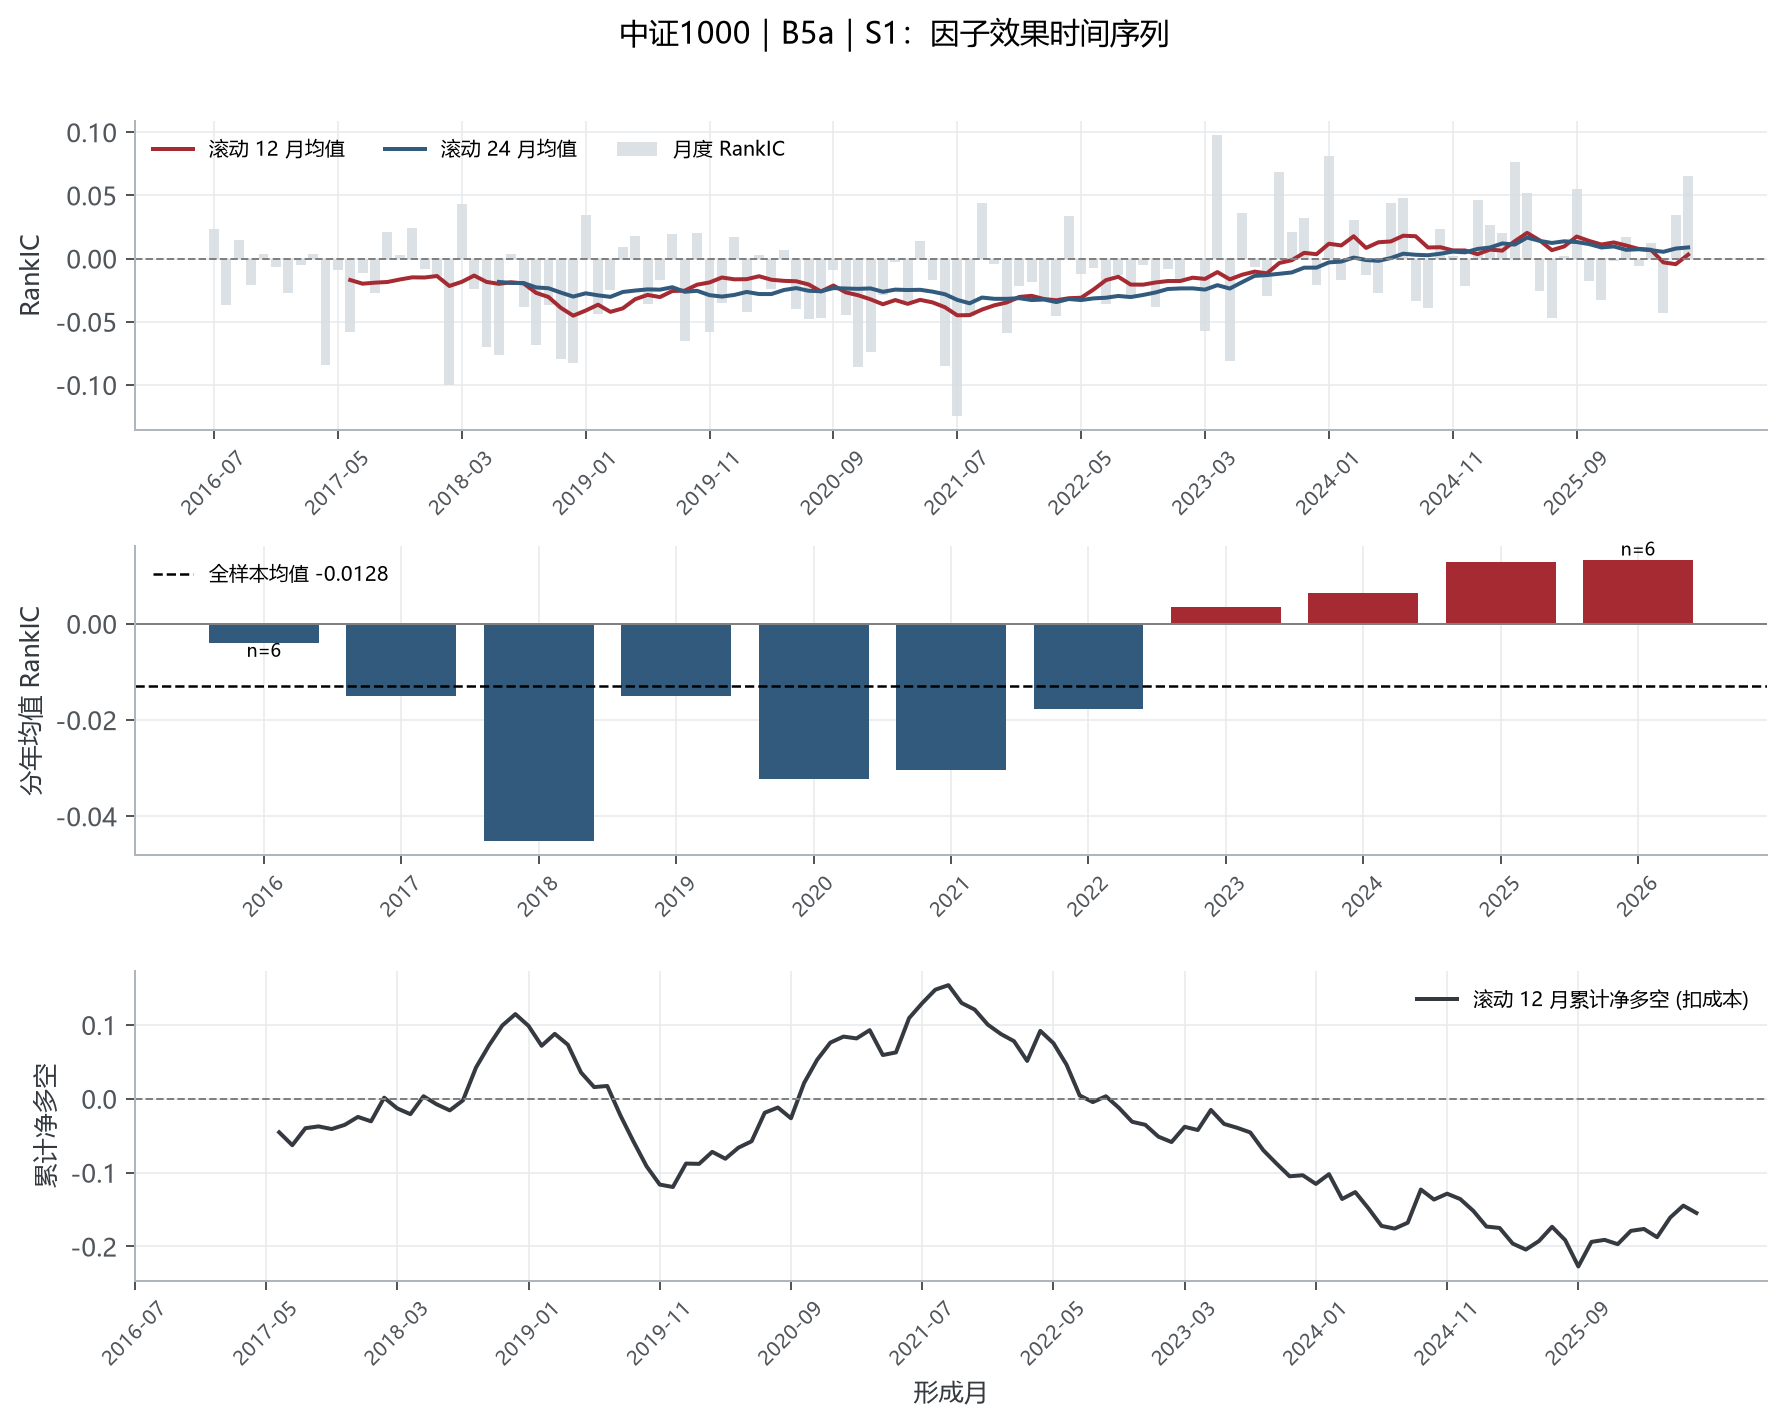
\includegraphics[width=.95\textwidth]{figs_v21/fig_3_4_zz1000_B5a_decay.png}
\caption*{\textbf{\textcolor{reportred}{图 3-4}}　中证1000 / B5a / S1：因子效果时间序列衰减（上：月度 RankIC 与 12/24 月滚动；中：分年 RankIC；下：滚动 12 月净多空）}
\end{figure}

\textbf{⑦ 模块小结}

``先后''（B1）与''极值点''（B5c）两个维度携带真实信息，且 B5c
的顶背离来源在量价中性后仍稳健（S2 RankICIR
−1.85\textasciitilde−2.44）；``上下力量对比''（B2/B2a）与''斜率背离''（B5b）在月度频率上不构成增量，条件化/交互项（B3/B4）虽在
S2 后增强但非独立来源------这是对模块 B
内部叙事的实证裁剪，\textbf{并非所有量价交互方向都值得构建因子}。

\begin{center}\rule{0.5\linewidth}{0.5pt}\end{center}

\section{四、模块
C：成交时序集中度类因子------信息到达的时间分布}\label{ux56dbux6a21ux5757-cux6210ux4ea4ux65f6ux5e8fux96c6ux4e2dux5ea6ux7c7bux56e0ux5b50ux4fe1ux606fux5230ux8fbeux7684ux65f6ux95f4ux5206ux5e03}

\subsection{4.1 构建动机}\label{ux6784ux5efaux52a8ux673a-2}

模块 C
旨在刻画\textbf{交易活动在时间轴上的分布形态，以及买卖两盘分布的差异}，对应微观结构中的''\textbf{信息到达模式}''：成交集中于少数分钟（低熵）=
离散的信息脉冲（公告、大单）；成交均匀分布（高熵）=
持续的价格发现。该维度与路径形状（模块 A）、量价方向（模块
B）正交------曲折度高的日子成交可集中亦可分散，领先滞后与成交时间分布无必然联系，故独立成模块。更进一步，\textbf{仅观察全天集中度的水平并不充分，买卖两盘的相对分布才携带主力行为信息}------买方脉冲式大单+卖方零星分散（吸筹）与卖方脉冲+买方分散（出货）在总集中度上无法区分，须按价格方向条件化。

\subsection{4.2
因子定义与计算方法}\label{ux56e0ux5b50ux5b9aux4e49ux4e0eux8ba1ux7b97ux65b9ux6cd5-2}

统一记号同前；另设上涨/下跌分钟量占比：

\[w_t^+=\frac{V_t\cdot\mathbb{1}\{r_t>0\}}{\sum_s V_s\cdot\mathbb{1}\{r_s>0\}},\qquad w_t^-=\frac{V_t\cdot\mathbb{1}\{r_t<0\}}{\sum_s V_s\cdot\mathbb{1}\{r_s<0\}}\]

以下按''数据变换 → K 线聚合''算子链给出，因子末端必为 K 线聚合（C1/C2 为
20 日均值、C3 为 20 日标准差）。

\textbf{C1 日内成交集中度熵因子}

\begin{enumerate}
\def\labelenumi{\arabic{enumi}.}
\tightlist
\item
  \textbf{数据变换}（除法）：分钟量占比 \(w_t=V_t/\sum_s V_s\)（日量合计
  \(\le0\) 处无定义）；
\item
  \textbf{K 线聚合}（熵）：日内熵 \(H=-\sum_t w_t\ln w_t\)（约定
  \(0\ln0=0\)，要求有量分钟 \(N\ge2\)）；
\item
  \textbf{数据变换}（除法）：标准化熵 \(H^*=H/\ln 240\)（以日内分钟数
  240 的对数归一化至 \([0,1]\)，保留成交稀疏度信息）；
\item
  \textbf{K 线聚合}（20 日均值）：\(F_{C1}=\mathrm{Mean}_{20d}(H^*)\)。
\end{enumerate}

\textbf{C2 买卖盘成交集中度差异因子}

\begin{enumerate}
\def\labelenumi{\arabic{enumi}.}
\tightlist
\item
  \textbf{数据变换}（0-1 化·除法）：上涨分钟量占比
  \(w_t^+\)、下跌分钟量占比 \(w_t^-\)（按 \(r_t\) 符号条件化）；
\item
  \textbf{K 线聚合}（熵）：上涨熵 \(H^+=-\sum_t w_t^+\ln w_t^+\)、下跌熵
  \(H^-\) 同理（两侧有量分钟均 \(\ge2\)）；
\item
  \textbf{数据变换}（减法）：集中度差 \(\Delta H=H^+-H^-\)；
\item
  \textbf{K 线聚合}（20
  日均值）：\(F_{C2}=\mathrm{Mean}_{20d}(\Delta H)\)。
\end{enumerate}

\textbf{C3 成交集中度变异因子}

\begin{enumerate}
\def\labelenumi{\arabic{enumi}.}
\tightlist
\item
  \textbf{K 线聚合}（20
  日标准差）：\(F_{C3}=\mathrm{Std}_{20d}(H^*)\)------对 C1
  的日度标准化熵取 20
  日\textbf{标准差}（非均值），刻画集中度在时间轴上的不稳定程度。
\end{enumerate}

\subsection{4.3
因子经济含义}\label{ux56e0ux5b50ux7ecfux6d4eux542bux4e49-2}

\begin{itemize}
\tightlist
\item
  \textbf{C1（基础成交集中度）}：\(H^*\approx1\)
  表明成交均匀分布于全天（信息连续到达、持续价格发现）；\(H^*\approx0\)
  表明成交集中于少数分钟（信息脉冲到达、事件/大单驱动）。以 \(\ln 240\)
  标准化至 \([0,1]\)，保留成交稀疏度信息。
\item
  \textbf{C2（买卖盘集中度差）}：\(\Delta H<0\)（上涨成交更集中）=
  买方脉冲式大单、卖方分散式零星 → 主力吸筹特征；\(\Delta H>0\) =
  卖方脉冲、买方分散 →
  出货特征。实证方向为正（上涨分散、下跌集中者未来跑赢），见 4.4。
\item
  \textbf{C3（集中度变异）}：集中度在 20
  日内的波动------信息到达模式不稳定、事件频发的市场状态，为 C1
  的二阶版本。
\end{itemize}

\subsection{4.4
因子表现评估}\label{ux56e0ux5b50ux8868ux73b0ux8bc4ux4f30-2}

\textbf{① 因子总览（RankICIR；同因子 S1 一行、S2
一行，横向对比四股票池）}

\begin{longtable}{@{}p{3.0cm} c r r r r p{5.2cm}@{}}
\caption{表 7　模块 C 因子总览（RankICIR，S1/S2 四池）}\\
\toprule
因子 & 中性化 & 沪深300 & 中证500 & 中证1000 & 中证全指 & 判读 \\
\midrule
\endfirsthead
\toprule
因子 & 中性化 & 沪深300 & 中证500 & 中证1000 & 中证全指 & 判读 \\
\midrule
\endhead
\bottomrule
\endfoot
\multirow{2}{\hsize}{\textbf{C1 集中度熵}} & S1 & 0.60 & −0.23 & −0.96 & −1.16 & \multirow{2}{\hsize}{水平信息有限，方向随池漂移} \\
 & S2 & 0.74 & 0.17 & −0.19 & −0.41 & \\
\cmidrule(lr){2-6}
\multirow{2}{\hsize}{\textbf{C2 买卖盘集中差}} & S1 & \textbf{1.19} & 1.64 & \textbf{2.26} & \textbf{2.55} & \multirow{2}{\hsize}{四池全显著、小盘最强；S2 后衰减最小（−18\%）} \\
 & S2 & 0.97 & 1.01 & 1.38 & 1.66 & \\
\cmidrule(lr){2-6}
\multirow{2}{\hsize}{\textbf{C3 集中度变异}} & S1 & −1.34 & −0.59 & −1.06 & −1.02 & \multirow{2}{\hsize}{中等负向；S2 后中证全指归零（−0.07）} \\
 & S2 & −0.93 & −0.01 & −0.38 & −0.07 & \\
\end{longtable}

\textbf{② C2（买卖盘集中度差）：模块 C 的核心增量}

\begin{itemize}
\tightlist
\item
  \textbf{方向与稳定性}：方向统一为正------\(\Delta H\)
  高（上涨成交更分散、下跌成交更集中）者未来跑赢，即''卖方脉冲、买方分散''（出货特征）跑输、``买方脉冲、卖方分散''（吸筹特征）跑赢，与主力行为叙事预期一致。中证1000
  分年 IC \textbf{全部 11 年为正}（2016H2 7.7\% → 2026H1
  1.9\%），时序稳定性极佳。
\end{itemize}

\begin{figure}[H]
\centering
\begin{minipage}[t]{0.49\textwidth}
\centering
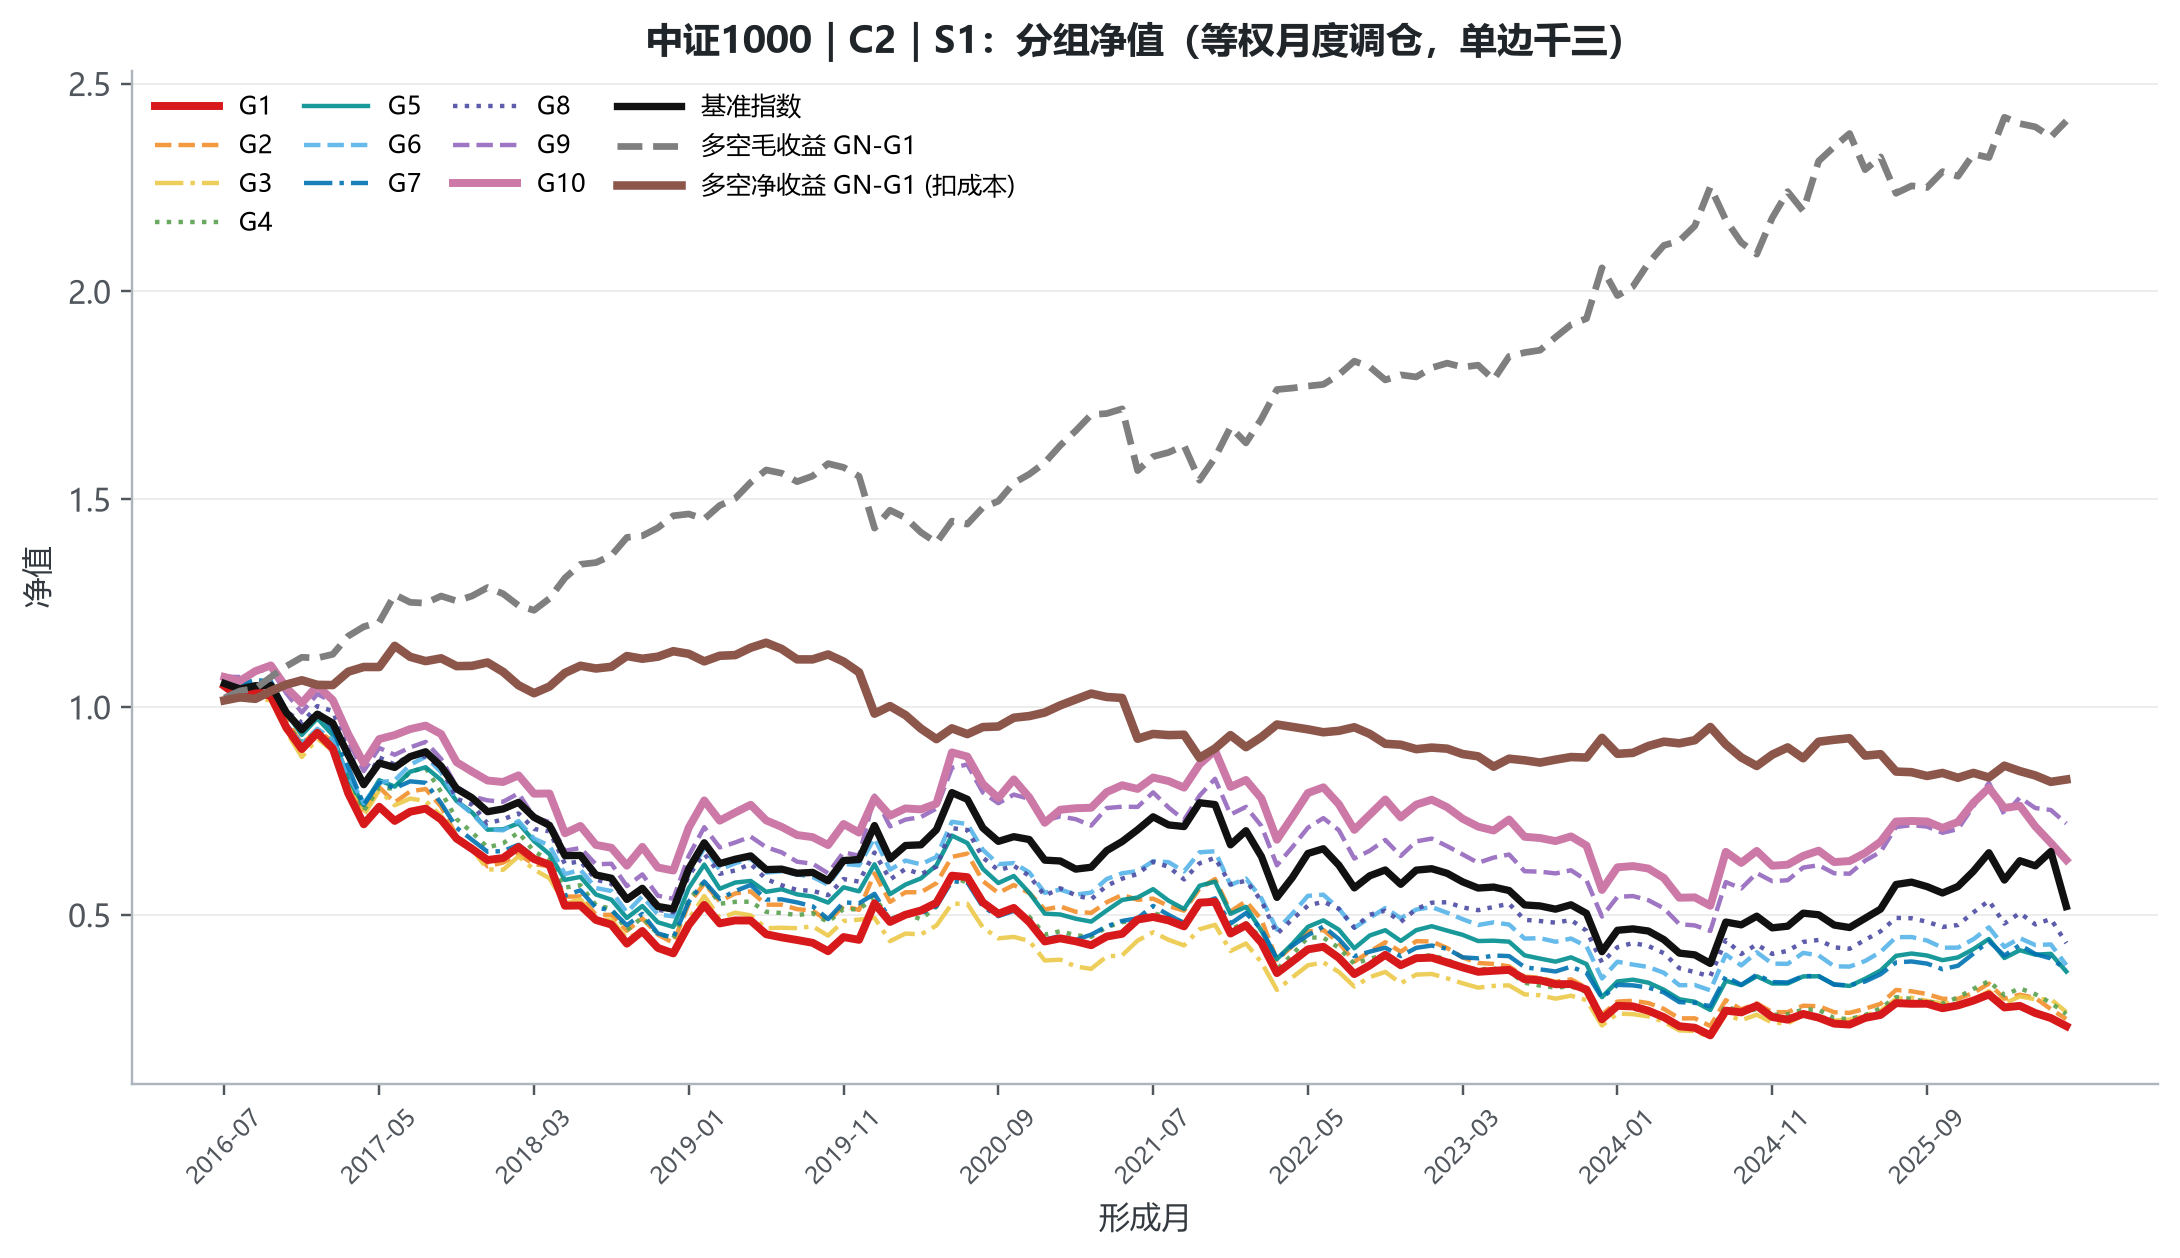
\includegraphics[width=\linewidth]{figs_v21/fig_4_1_zz1000_C2_group_nav.png}
\vspace{2pt}\caption*{\textbf{\textcolor{reportred}{图 4-1}}　中证1000 / C2 / S1：分组净值（$G\_1$ −13.8\% → $G\_\{10\}$ −4.8\%，毛多空 +9.2\%）}
\end{minipage}\hfill
\begin{minipage}[t]{0.49\textwidth}
\centering
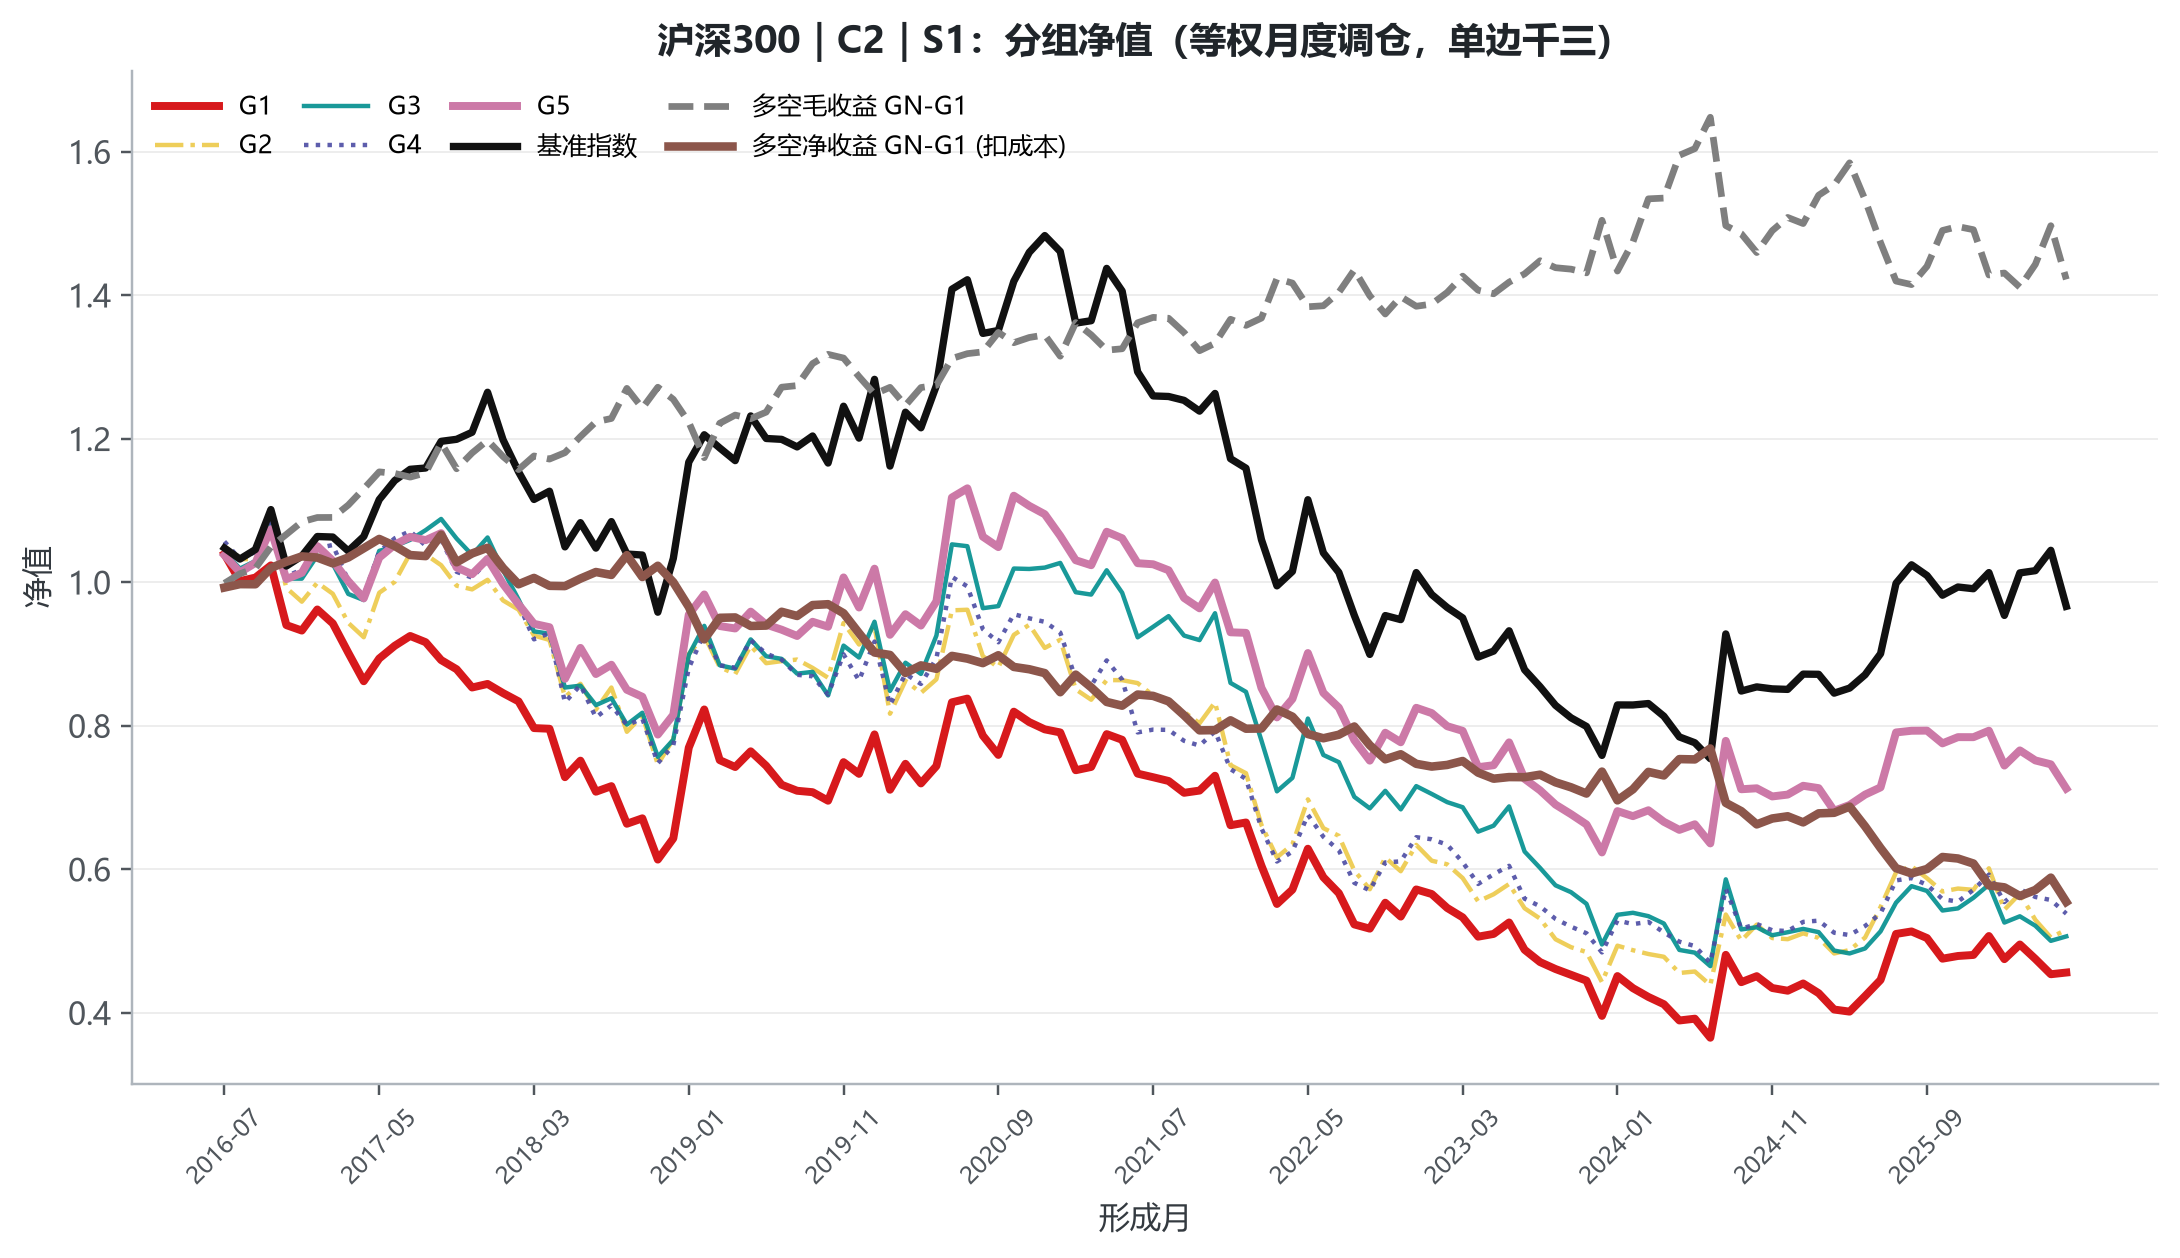
\includegraphics[width=\linewidth]{figs_v21/fig_4_2_hs300_C2_group_nav.png}
\vspace{2pt}\caption*{\textbf{\textcolor{reportred}{图 4-2}}　沪深300 / C2 / S1：分组净值（大盘域亦稳健，毛多空 +3.6\%）}
\end{minipage}
\end{figure}

\begin{itemize}
\tightlist
\item
  \textbf{S1 与 S2 对照}：沪深300
  1.19→0.97（−18\%，\textbf{全体系衰减最小}）、中证1000
  2.26→1.38（−39\%）、中证全指 2.55→1.66------对比 A3 在中证1000 由 3.30
  降至 1.83（−45\%），C2
  的收益来源\textbf{较少借自换手率/波动率暴露}，更接近独立的信息到达模式维度，是''干净增量''的样板。
\item
  \textbf{时序衰减}：前后半 ICIR 中证1000 2.38→2.18、中证全指
  2.79→2.49、沪深300 1.46→0.99，各池轻度衰减；2025 年以来月均 RankIC
  +2.3\%\textasciitilde+5.3\%（方向胜率
  61\%\textasciitilde72\%）------最干净的增量来源在时序上同样未实质衰减。
\end{itemize}

\begin{figure}[H]
\centering
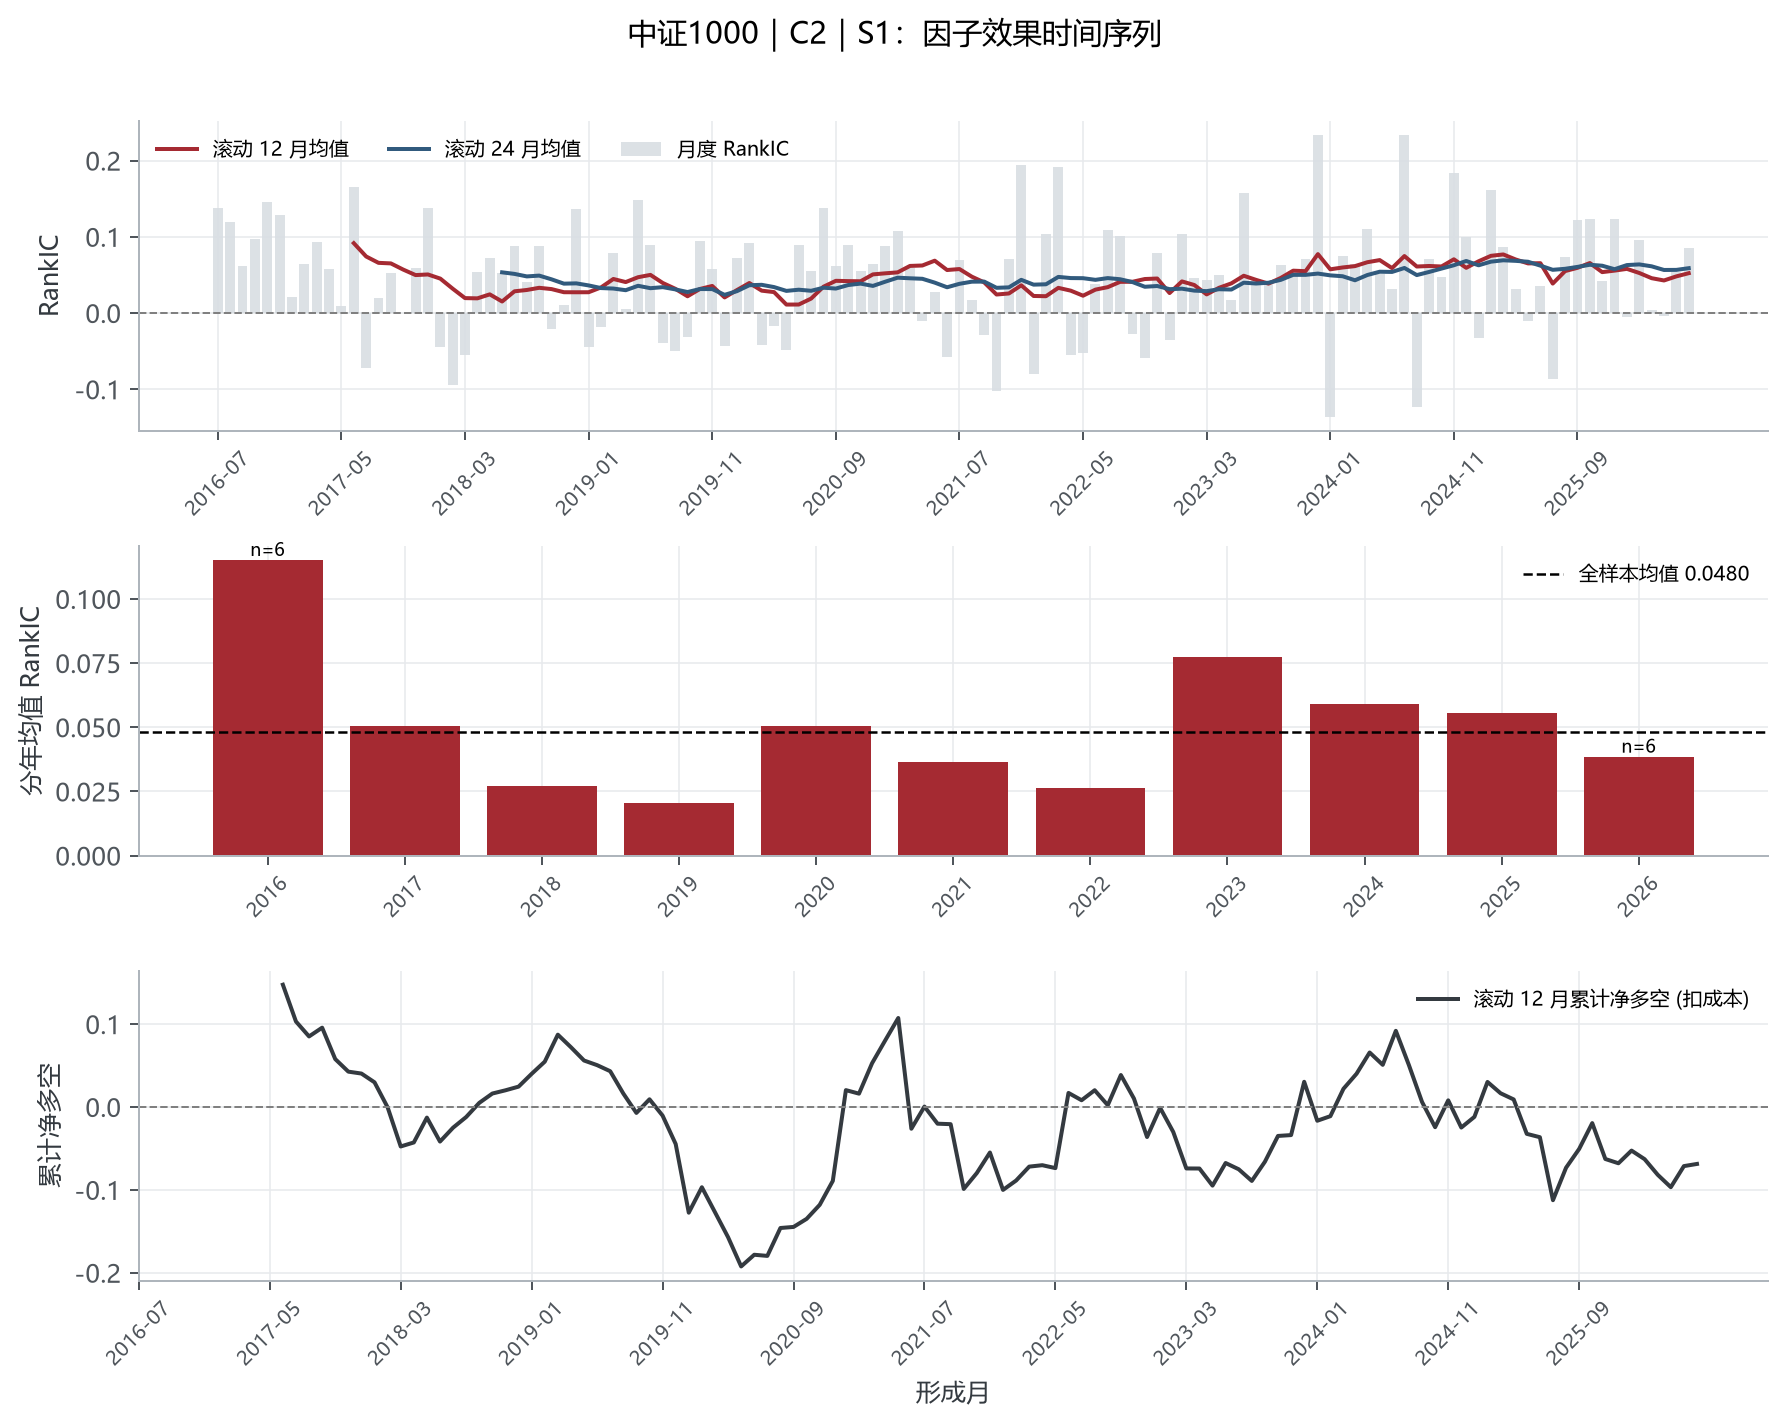
\includegraphics[width=.95\textwidth]{figs_v21/fig_4_3_zz1000_C2_decay.png}
\caption*{\textbf{\textcolor{reportred}{图 4-3}}　中证1000 / C2 / S1：因子效果时间序列衰减（上：月度 RankIC 与 12/24 月滚动；中：分年 RankIC；下：滚动 12 月净多空）}
\end{figure}

\textbf{③ C1（水平）与 C3（波动）：信息有限}

\begin{itemize}
\tightlist
\item
  \textbf{C1}：S1 方向在四池间漂移（沪深300 +0.60、中证1000
  −0.96），\textbf{S2 后 \textbar RankICIR\textbar{} 均降至 0.75
  以下}（中证全指 −1.16→−0.41），不构成稳健来源。
\item
  \textbf{C3}：S1 中证1000/中证全指 −1.06/−1.02，\textbf{S2 后降至
  −0.38/−0.07 基本归零}------集中度的波动信息同样借自量价暴露。
\item
  两者共同印证模块 C
  的核心判断：\textbf{集中度的绝对水平与波动不携带月度选股信息，买卖两盘的相对分布才携带主力行为信息}。
\item
  \textbf{时序衰减}：两者分化------C1
  后半幅度略衰且方向跨池漂移（沪深300 +0.76→+0.41、中证1000
  −1.07→−0.84），无稳定结论；C3 则负向增强（中证全指前半 ICIR −0.58 →
  后半 −1.87、中证1000 −0.75→−1.61），2025 年以来月均 RankIC
  −3.4\%/−3.5\%（方向胜率均 78\%）------集中度波动信息近年才显现，与 A3
  的衰减形成镜像对照。
\end{itemize}

\begin{figure}[H]
\centering
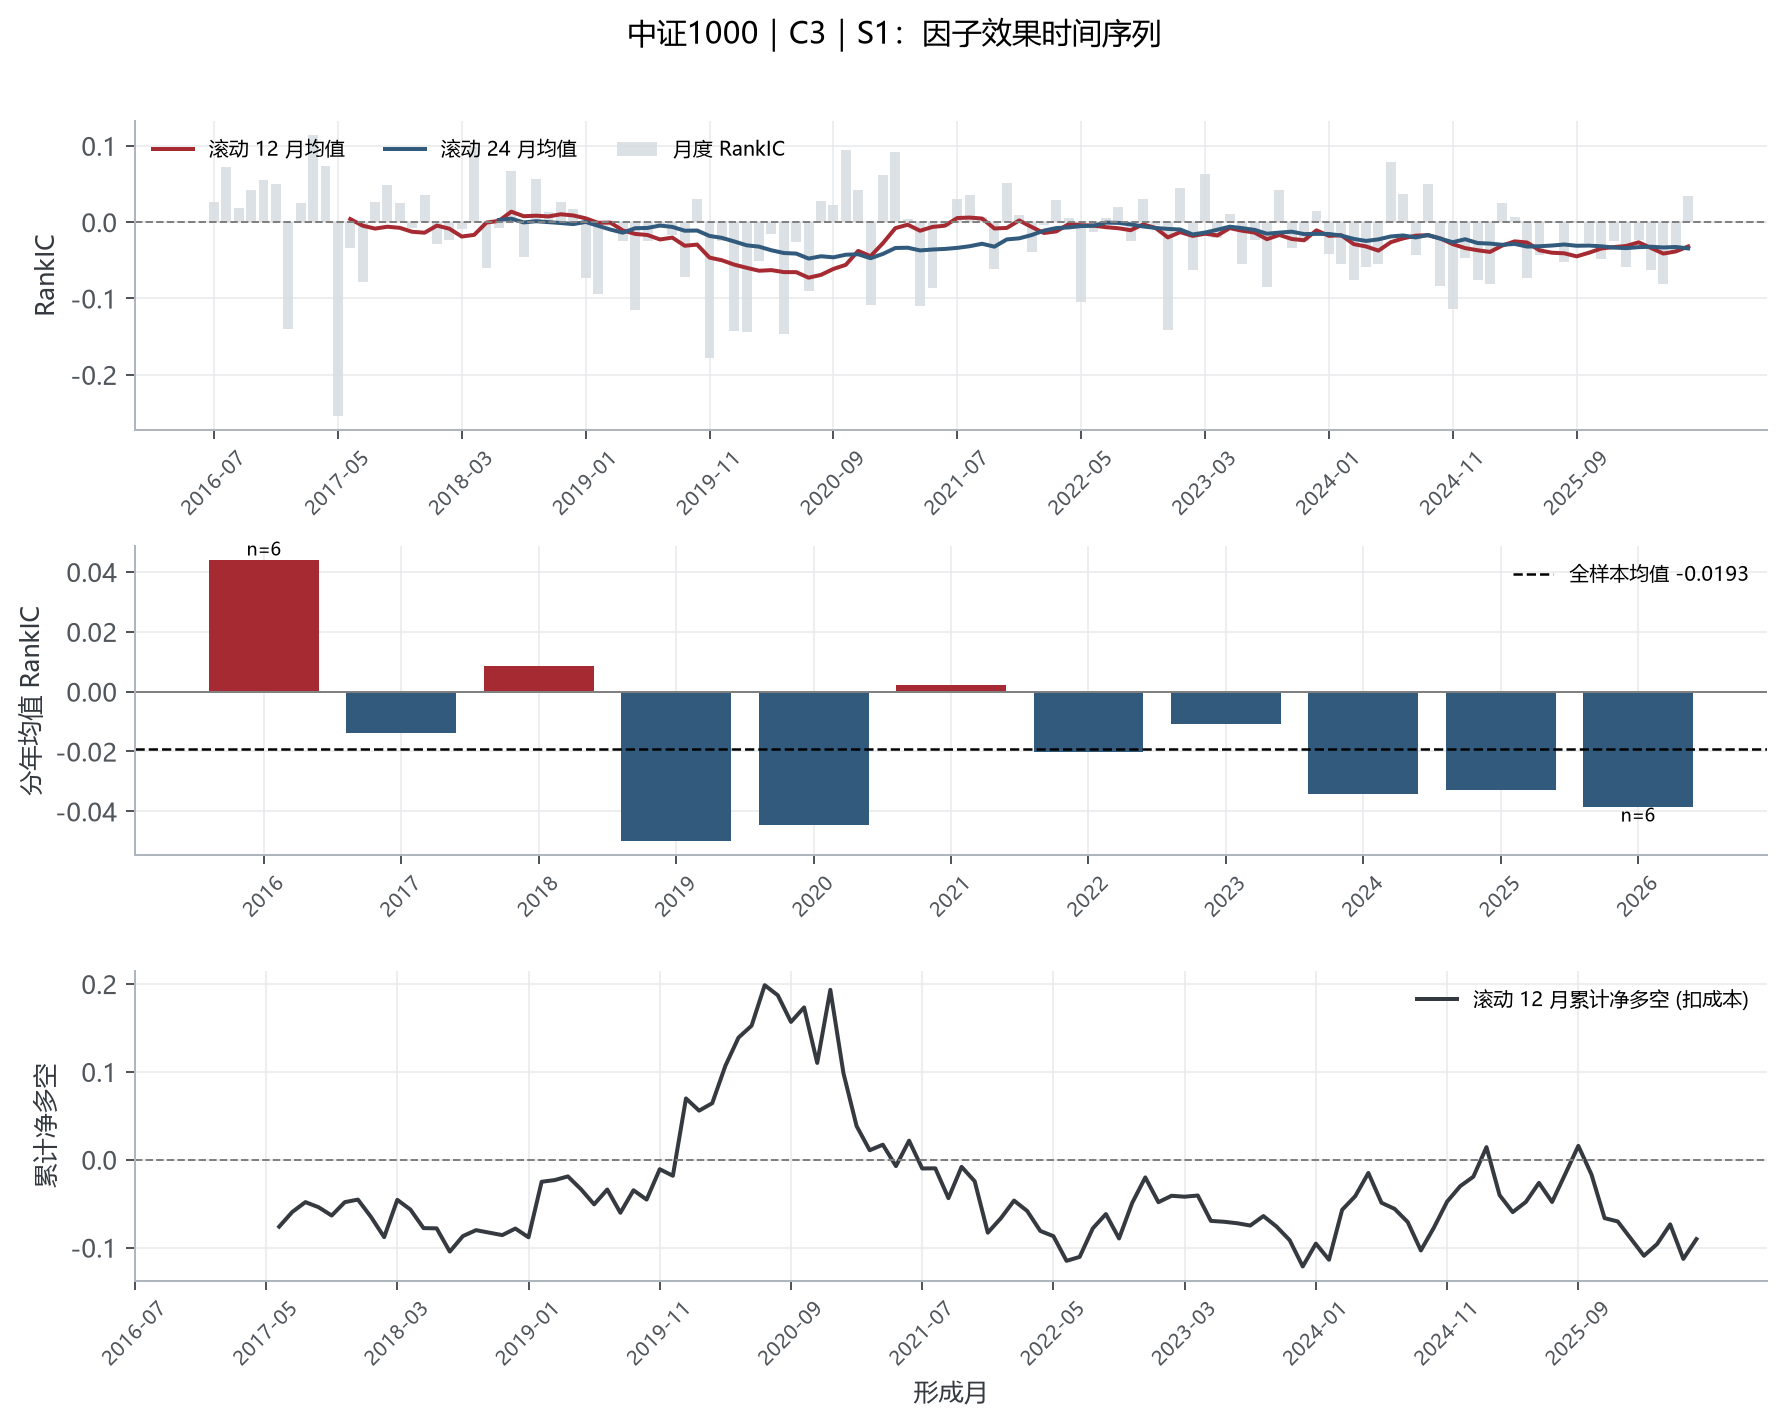
\includegraphics[width=.95\textwidth]{figs_v21/fig_4_4_zz1000_C3_decay.png}
\caption*{\textbf{\textcolor{reportred}{图 4-4}}　中证1000 / C3 / S1：因子效果时间序列衰减（上：月度 RankIC 与 12/24 月滚动；中：分年 RankIC；下：滚动 12 月净多空）}
\end{figure}

\textbf{④ 模块小结}

条件化是 C 模块的关键------从 C1（全池偏弱）到
C2（四池全显著、量价中性后最稳）的跃升，为''切割/条件化分离相反逻辑即得增量''的又一例证；C2
与 B5c 一并构成本体系中最接近独立维度的两个增量来源。

\begin{center}\rule{0.5\linewidth}{0.5pt}\end{center}

\section{五、整体实证结果与深度分析}\label{ux4e94ux6574ux4f53ux5b9eux8bc1ux7ed3ux679cux4e0eux6df1ux5ea6ux5206ux6790}

\subsection{5.1 144 组回测总览}\label{ux7ec4ux56deux6d4bux603bux89c8}

S1 口径下 \textbar RankICIR\textbar{} \textgreater{} 1 的组合共 36
个（占 72 个''池×因子''组合的一半）。全部 18 因子 × 4 池的 RankICIR
全景见图 5-1：

\begin{figure}[H]
\centering
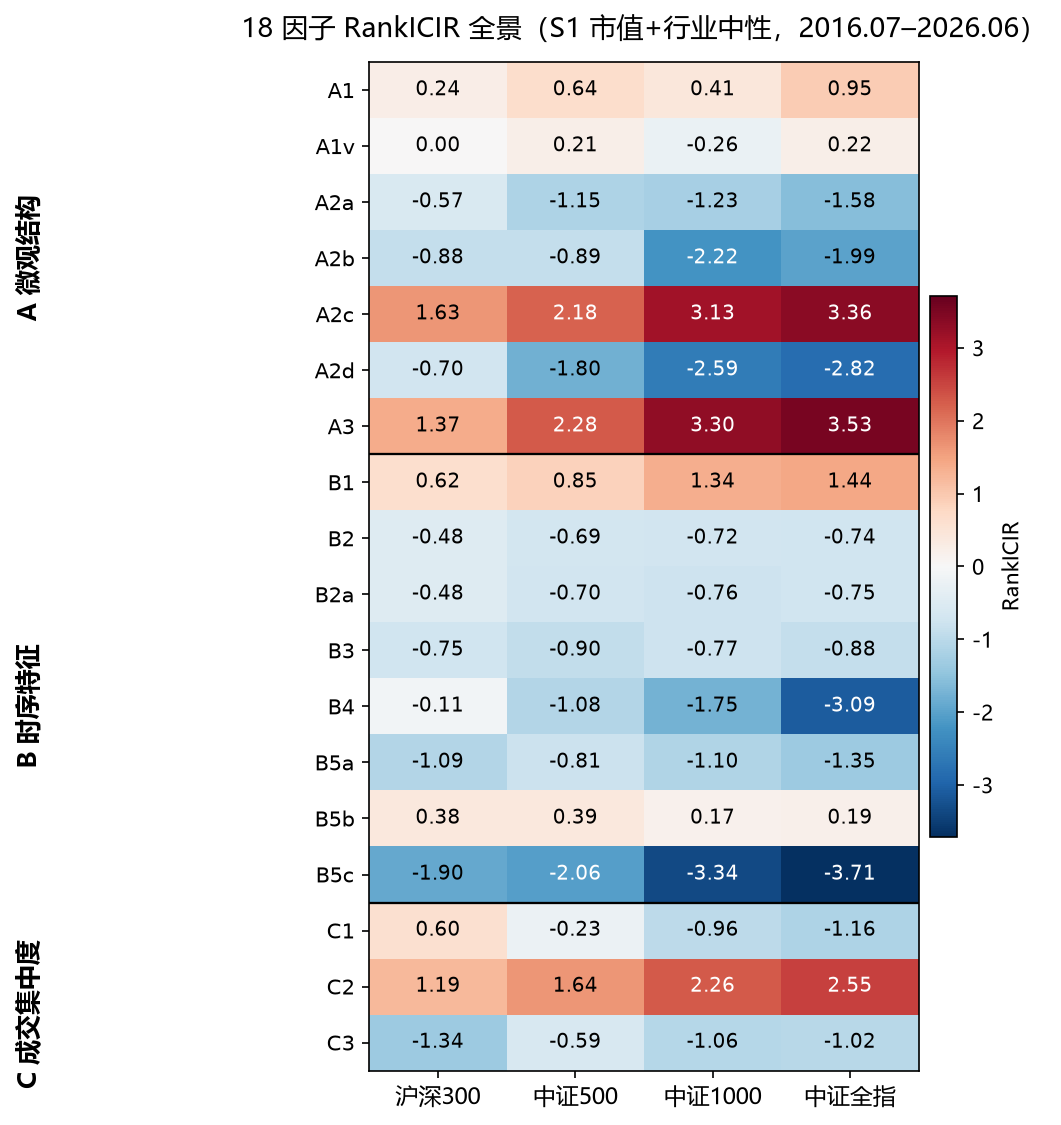
\includegraphics[width=.95\textwidth]{figs_v21/fig_5_1_rankicir_heatmap.png}
\caption*{\textbf{\textcolor{reportred}{图 5-1}}　18 因子 RankICIR 全景热力图（S1 市值+行业中性，2016.07–2026.06；红色为正、蓝色为负）}
\end{figure}

为便于直接比较''同一因子在不同市场的表现、以及叠加量价中性（S2）后的变化''，图
5-2 将 18 因子按''S1 一行 / S2 一行''排布、横向对照四股票池：

\begin{figure}[H]
\centering
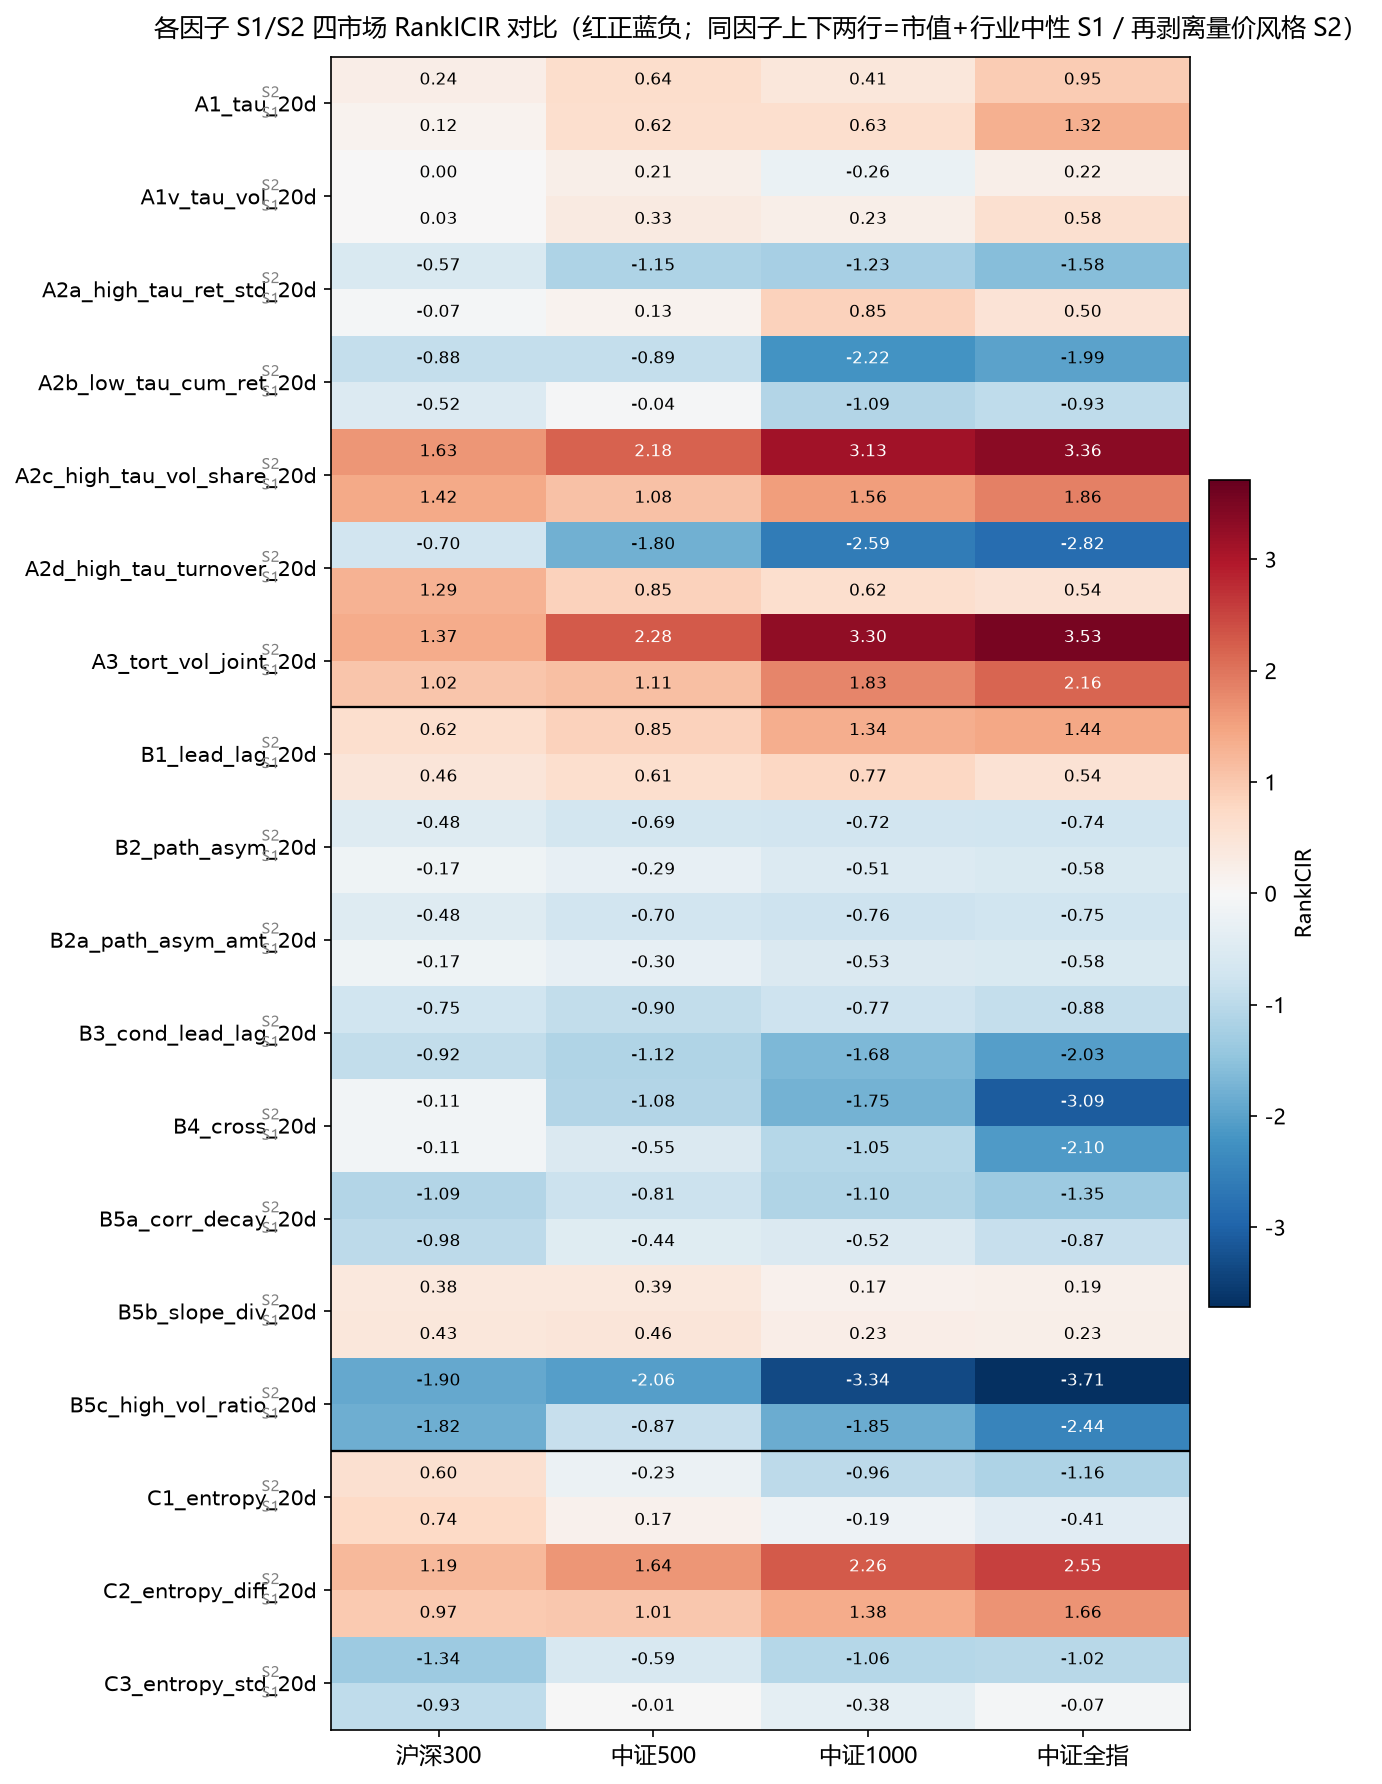
\includegraphics[width=.95\textwidth]{figs_v21/fig_5_4_market_s1s2.png}
\caption*{\textbf{\textcolor{reportred}{图 5-2}}　各因子 S1/S2 四市场 RankICIR 对比（同因子上下两行 = S1 市值+行业中性 / S2 再剥离换手+波动；红正蓝负）}
\end{figure}

从热力图可归纳四条结构性信息：

\begin{enumerate}
\def\labelenumi{\arabic{enumi}.}
\tightlist
\item
  \textbf{最强四个因子为
  A3、A2c、C2、B5c}（红色最深），且在中证1000/中证全指两个小盘域最为突出；
\item
  \textbf{模块 A 整体最强、模块 C 由 C2 一枝独秀、模块 B
  内部两极分化}（B5c 深蓝、B1 浅红、B2/B5b 近乎无色）；
\item
  \textbf{沪深300 一列整体颜色最浅}------所有因子在大盘域大幅衰减；
\item
  \textbf{同一因子两池之间的热力梯度}（如 A2c 自 hs300 1.63 至 zzall
  3.36）提示''域敏感性''为普遍规律。
\end{enumerate}

\subsection{5.2 风格相关性定位：18 因子 × 9
风格的收益来源归属}\label{ux98ceux683cux76f8ux5173ux6027ux5b9aux4f4d18-ux56e0ux5b50-9-ux98ceux683cux7684ux6536ux76caux6765ux6e90ux5f52ux5c5e}

在补全风格暴露数据后（量价类 5 风格由本地日频缓存自建，财务类
BP/DP/成长/盈利由天软补全至 2026-06；与 F 盘 \texttt{table\_yuanshi.pkl}
2016-07\textasciitilde2023-11
重叠期交叉验证：规模/波动/换手/反转/动量/BP/盈利相关系数
0.89\textasciitilde1.00，成长受 F 盘利润增速极端值影响 Pearson 失真但
Spearman 0.39
有效，见附录），补上六步检验法的第一步。下表为中证全指内，\textbf{S1
残差口径下} 18 因子与 9 风格的月度截面相关系数（时序均值）：

\begin{longtable}[]{@{}
  >{\raggedright\arraybackslash}p{(\linewidth - 18\tabcolsep) * \real{0.1000}}
  >{\raggedright\arraybackslash}p{(\linewidth - 18\tabcolsep) * \real{0.1000}}
  >{\raggedright\arraybackslash}p{(\linewidth - 18\tabcolsep) * \real{0.1000}}
  >{\raggedright\arraybackslash}p{(\linewidth - 18\tabcolsep) * \real{0.1000}}
  >{\raggedright\arraybackslash}p{(\linewidth - 18\tabcolsep) * \real{0.1000}}
  >{\raggedright\arraybackslash}p{(\linewidth - 18\tabcolsep) * \real{0.1000}}
  >{\raggedright\arraybackslash}p{(\linewidth - 18\tabcolsep) * \real{0.1000}}
  >{\raggedright\arraybackslash}p{(\linewidth - 18\tabcolsep) * \real{0.1000}}
  >{\raggedright\arraybackslash}p{(\linewidth - 18\tabcolsep) * \real{0.1000}}
  >{\raggedright\arraybackslash}p{(\linewidth - 18\tabcolsep) * \real{0.1000}}@{}}
\caption{表 8　18 因子 × 9 风格相关系数（S1
残差，中证全指）}\tabularnewline
\toprule\noalign{}
\begin{minipage}[b]{\linewidth}\raggedright
因子
\end{minipage} & \begin{minipage}[b]{\linewidth}\raggedright
波动率
\end{minipage} & \begin{minipage}[b]{\linewidth}\raggedright
换手率
\end{minipage} & \begin{minipage}[b]{\linewidth}\raggedright
动量
\end{minipage} & \begin{minipage}[b]{\linewidth}\raggedright
反转
\end{minipage} & \begin{minipage}[b]{\linewidth}\raggedright
BP
\end{minipage} & \begin{minipage}[b]{\linewidth}\raggedright
DP
\end{minipage} & \begin{minipage}[b]{\linewidth}\raggedright
成长
\end{minipage} & \begin{minipage}[b]{\linewidth}\raggedright
盈利
\end{minipage} & \begin{minipage}[b]{\linewidth}\raggedright
判读
\end{minipage} \\
\midrule\noalign{}
\endfirsthead
\toprule\noalign{}
\begin{minipage}[b]{\linewidth}\raggedright
因子
\end{minipage} & \begin{minipage}[b]{\linewidth}\raggedright
波动率
\end{minipage} & \begin{minipage}[b]{\linewidth}\raggedright
换手率
\end{minipage} & \begin{minipage}[b]{\linewidth}\raggedright
动量
\end{minipage} & \begin{minipage}[b]{\linewidth}\raggedright
反转
\end{minipage} & \begin{minipage}[b]{\linewidth}\raggedright
BP
\end{minipage} & \begin{minipage}[b]{\linewidth}\raggedright
DP
\end{minipage} & \begin{minipage}[b]{\linewidth}\raggedright
成长
\end{minipage} & \begin{minipage}[b]{\linewidth}\raggedright
盈利
\end{minipage} & \begin{minipage}[b]{\linewidth}\raggedright
判读
\end{minipage} \\
\midrule\noalign{}
\endhead
\bottomrule\noalign{}
\endlastfoot
A1 基础曲折度 & −0.01 & +0.03 & +0.07 & +0.03 & −0.08 & −0.02 & +0.02 &
+0.02 & 基本无风格暴露 \\
A2a 噪音强度 & \textbf{+0.47} & +0.33 & +0.16 & +0.24 & −0.02 & −0.19 &
+0.00 & −0.08 & 高波来源 \\
A2b 低曲折收益 & +0.21 & +0.17 & +0.07 & \textbf{+0.36} & −0.18 & +0.01
& +0.02 & +0.04 & 反转来源 \\
A2c 高曲折集中 & \textbf{−0.53} & \textbf{−0.45} & −0.11 & −0.18 & +0.14
& +0.15 & −0.01 & +0.04 & 低波低换手 \\
A2d 高曲折换手 & +0.56 & \textbf{+0.87} & +0.23 & +0.16 & −0.18 & −0.11
& +0.03 & −0.00 & \textbf{本质换手因子} \\
A3 曲折放量共振 & \textbf{−0.53} & \textbf{−0.52} & −0.15 & −0.18 &
+0.17 & +0.13 & −0.02 & +0.03 & 低波低换手+轻度价值 \\
B1 领先滞后 & −0.07 & −0.10 & −0.01 & +0.10 & −0.00 & −0.01 & −0.00 &
−0.00 & 暴露低 \\
B2/B2a 不对称 & +0.07 & +0.01 & −0.04 & +0.33 & −0.02 & −0.06 & −0.01 &
−0.04 & 轻度反转 \\
B5a 确认衰减 & +0.03 & +0.04 & +0.03 & −0.04 & −0.02 & −0.01 & −0.00 &
+0.00 & 暴露低 \\
B5b 斜率背离 & −0.01 & +0.01 & +0.01 & \textbf{+0.29} & +0.01 & +0.05 &
−0.00 & +0.02 & 反转来源 \\
B5c 新高量能 & +0.38 & +0.30 & +0.09 & +0.21 & \textbf{−0.19} & −0.14 &
+0.02 & −0.04 & 高波高换手+低价值 \\
C1 集中度熵 & +0.10 & +0.20 & +0.11 & −0.14 & −0.14 & +0.03 & +0.03 &
+0.05 & 暴露弱 \\
C2 买卖盘集中差 & −0.14 & −0.16 & −0.10 & +0.04 & \textbf{+0.20} & +0.10
& −0.01 & −0.00 & ** \\
C3 集中度变异 & +0.19 & +0.07 & −0.01 & +0.17 & −0.00 & −0.03 & −0.01 &
−0.03 & 暴露弱 \\
\end{longtable}

\begin{figure}[H]
\centering
\begin{minipage}[t]{0.49\textwidth}
\centering
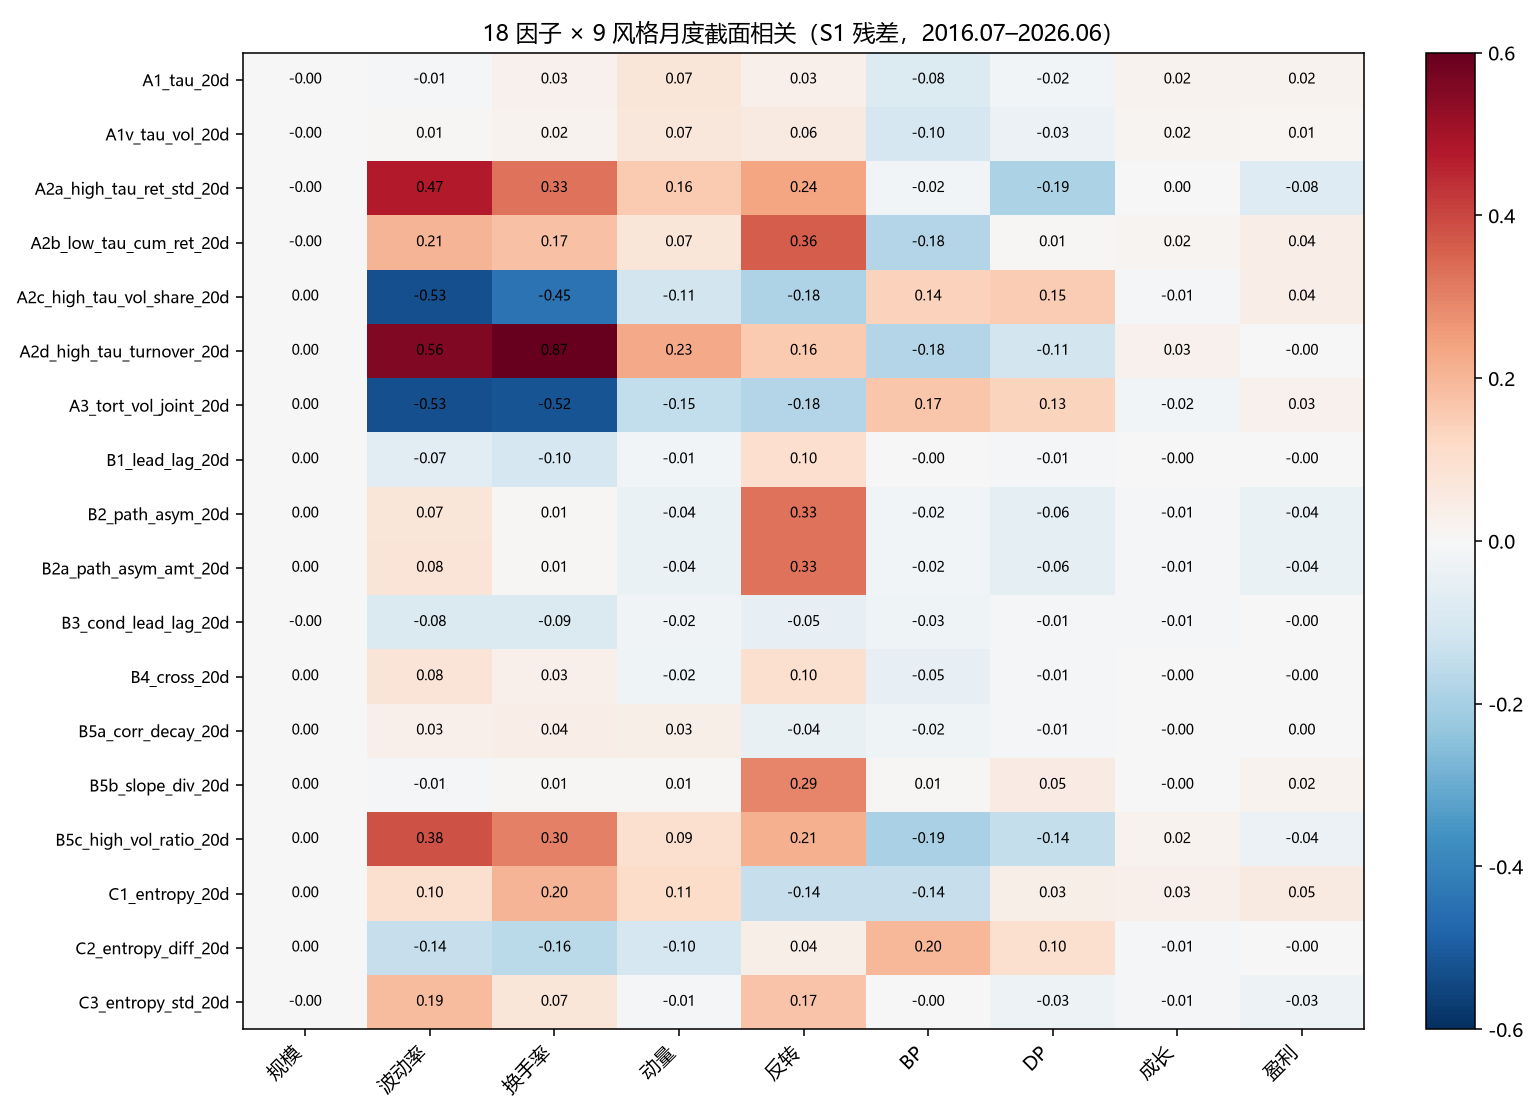
\includegraphics[width=\linewidth]{figs_v21/fig_5_2_style_corr.png}
\vspace{2pt}\caption*{\textbf{\textcolor{reportred}{图 5-3}}　18 因子 × 9 风格相关矩阵热力图（S1 残差，中证全指）}
\end{minipage}\hfill
\begin{minipage}[t]{0.49\textwidth}
\centering
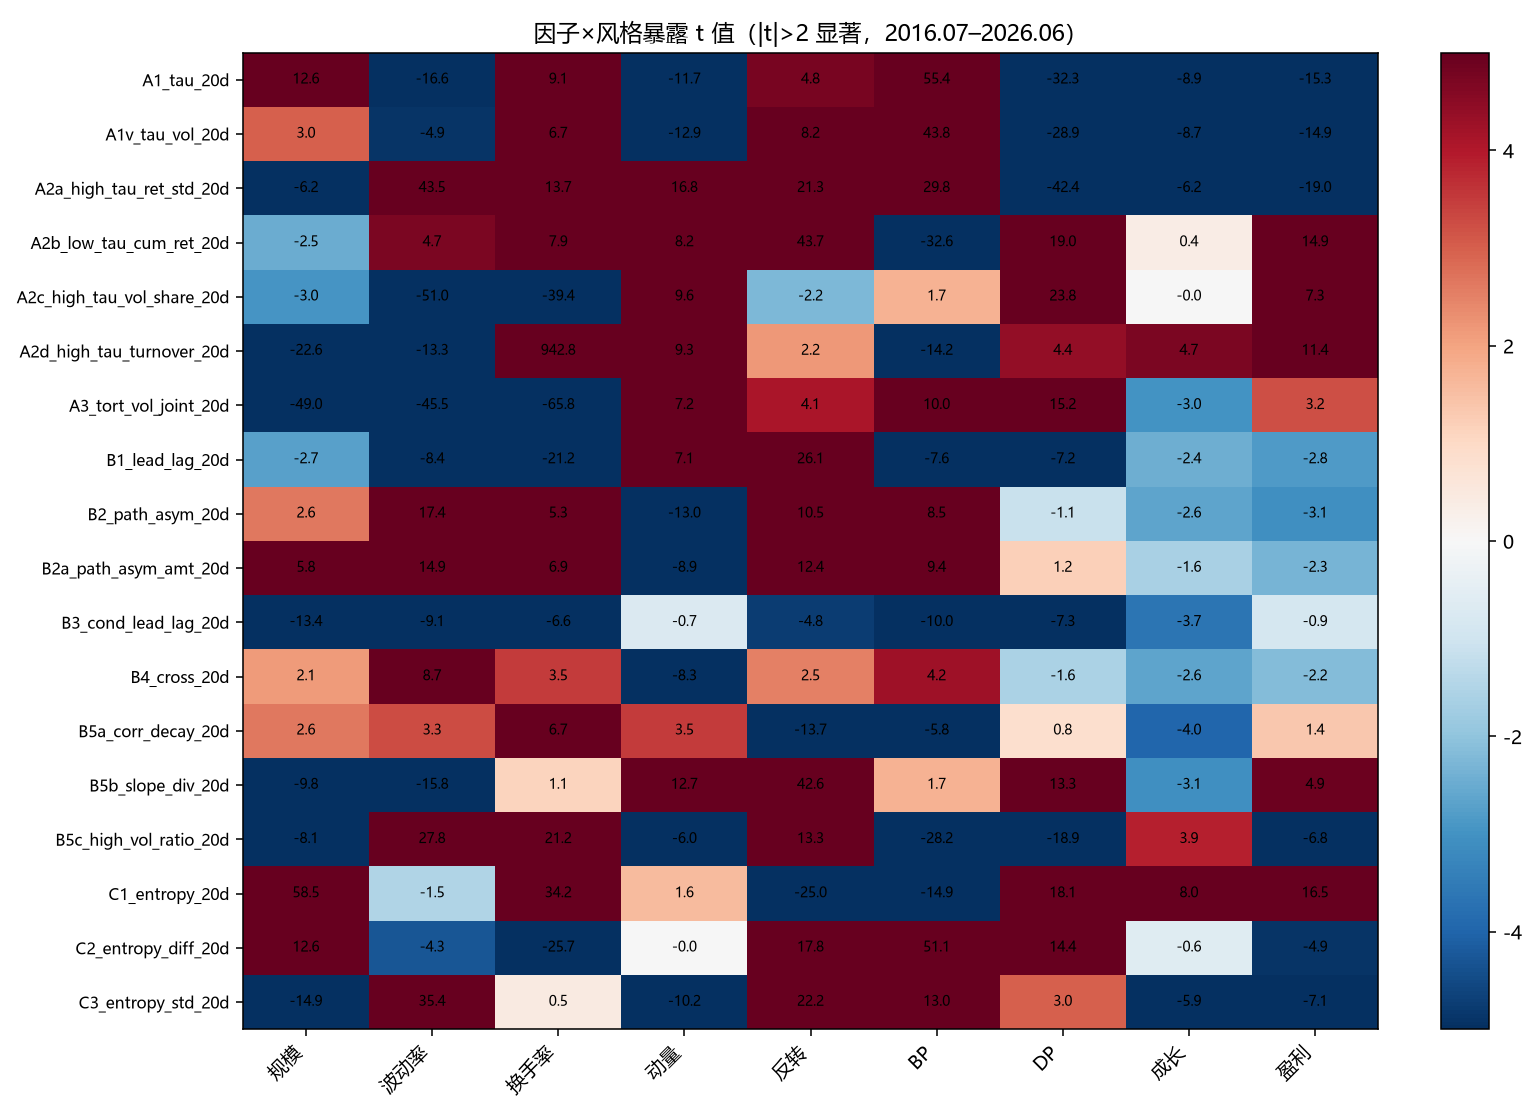
\includegraphics[width=\linewidth]{figs_v21/fig_5_3_exposure_tvals.png}
\vspace{2pt}\caption*{\textbf{\textcolor{reportred}{图 5-4}}　因子×风格暴露回归 t 值热力图}
\end{minipage}
\end{figure}

三条关键读数：

\begin{enumerate}
\def\labelenumi{\arabic{enumi}.}
\tightlist
\item
  \textbf{模块 A 的强因子确系''低波+低换手''来源}：A3/A2c
  与波动率（−0.53）、换手率（−0.52/−0.45）强负相关，与价值类风格（BP
  +0.17/+0.14、DP
  +0.13/+0.15）弱正------``低波低换手+轻度价值''的复合暴露；\textbf{A2d
  与换手率相关高达 +0.87（暴露回归
  β≈0.99），本质就是换手因子的另一种表达}，这解释了其 S2
  中性化后方向翻转。这与 5.4 节 S1→S2→S3 的落差结论互相印证：模块 A
  强信号的暴露全部集中在波动/换手，而非价值/动量/盈利。
\item
  \textbf{模块 B 内部分化}：A2a 偏波动（+0.47）、A2b
  偏反转（+0.36）、B5c 偏高波高换手（+0.38/+0.30）、B5b
  偏反转（+0.29），而 B1/B5a
  与各风格相关均低（\textbar corr\textbar\textless0.15）------这与''B5c/B1
  是独立时序信号、B2 是无效上下对比''的判断一致。
\item
  \textbf{C2 是体系中最干净的因子}：与全部 9 风格
  \textbar corr\textbar\textless0.2（最高为 BP +0.20、换手
  −0.16），几乎不携带任何风格暴露，与其''最干净增量''的定位完全一致；C1
  偏大市值（暴露回归规模 β +0.53），C3 偏波动（+0.19）。
\end{enumerate}

\subsection{5.3 结构性结论}\label{ux7ed3ux6784ux6027ux7ed3ux8bba}

\textbf{① 切割与交叉带来跃升（结构优于总量）。}
A1（0.24\textasciitilde0.95）→
A2c/A3（1.6\textasciitilde3.5）、C1（弱）→
C2（1.19\textasciitilde2.55）的跃升，验证''总量→结构→交叉''的递进设计：\textbf{时间段切割必须分离经济含义相反的状态才产生增量}（模块
A/C 的切割成功，B2 的''上下切割''失败）；时间点划分则适合捕捉价格新高等稀疏事件（B5c）。

\textbf{② 域敏感性是普遍规律。} 几乎所有因子在沪深300
大幅衰减、在中证1000/中证全指最强------路径形态信息主要存在于\textbf{小盘、高噪音域}，与''大盘股定价效率高、微观结构异象弱''的常识一致；本体系因子适用域天然偏小盘，入组合时应与小市值/流动性约束一并评估。

\textbf{③ 无效因子同样具有结论价值。} B2/B2a/B5b
的失败表明''上下力量对比''与''量价趋势同向性''在月度频率上不构成可交易信息；C1/C3
的失败表明''集中度的水平与波动''不携带信息------这些负面结果裁剪了因子库、避免无效信号堆叠，为收益来源导向研究的标准产出。

\subsection{5.4 稳健性：S1 / S2 / S3
中性化对照（量价中性与九风格试金石）}\label{ux7a33ux5065ux6027s1-s2-s3-ux4e2dux6027ux5316ux5bf9ux7167ux91cfux4ef7ux4e2dux6027ux4e0eux4e5dux98ceux683cux8bd5ux91d1ux77f3}

\begin{longtable}[]{@{}
  >{\raggedright\arraybackslash}p{(\linewidth - 12\tabcolsep) * \real{0.1429}}
  >{\raggedright\arraybackslash}p{(\linewidth - 12\tabcolsep) * \real{0.1429}}
  >{\raggedright\arraybackslash}p{(\linewidth - 12\tabcolsep) * \real{0.1429}}
  >{\raggedright\arraybackslash}p{(\linewidth - 12\tabcolsep) * \real{0.1429}}
  >{\raggedright\arraybackslash}p{(\linewidth - 12\tabcolsep) * \real{0.1429}}
  >{\raggedright\arraybackslash}p{(\linewidth - 12\tabcolsep) * \real{0.1429}}
  >{\raggedright\arraybackslash}p{(\linewidth - 12\tabcolsep) * \real{0.1429}}@{}}
\caption{表 9　S1 / S2 / S3 中性化对照（RankICIR）}\tabularnewline
\toprule\noalign{}
\begin{minipage}[b]{\linewidth}\raggedright
组合（RankICIR）
\end{minipage} & \begin{minipage}[b]{\linewidth}\raggedright
S1
\end{minipage} & \begin{minipage}[b]{\linewidth}\raggedright
S2
\end{minipage} & \begin{minipage}[b]{\linewidth}\raggedright
S3
\end{minipage} & \begin{minipage}[b]{\linewidth}\raggedright
S2 落差
\end{minipage} & \begin{minipage}[b]{\linewidth}\raggedright
S3 落差
\end{minipage} & \begin{minipage}[b]{\linewidth}\raggedright
判读
\end{minipage} \\
\midrule\noalign{}
\endfirsthead
\toprule\noalign{}
\begin{minipage}[b]{\linewidth}\raggedright
组合（RankICIR）
\end{minipage} & \begin{minipage}[b]{\linewidth}\raggedright
S1
\end{minipage} & \begin{minipage}[b]{\linewidth}\raggedright
S2
\end{minipage} & \begin{minipage}[b]{\linewidth}\raggedright
S3
\end{minipage} & \begin{minipage}[b]{\linewidth}\raggedright
S2 落差
\end{minipage} & \begin{minipage}[b]{\linewidth}\raggedright
S3 落差
\end{minipage} & \begin{minipage}[b]{\linewidth}\raggedright
判读
\end{minipage} \\
\midrule\noalign{}
\endhead
\bottomrule\noalign{}
\endlastfoot
中证1000 / A3 & 3.30 & 1.83 & 1.80 & −45\% & −2\% &
暴露几乎全在波动/换手 \\
中证1000 / A2c & 3.13 & 1.56 & 1.63 & −50\% & +4\% & S3 微升 \\
中证1000 / C2 & 2.26 & 1.38 & 1.50 & −39\% & +9\% & S3 修复 \\
中证1000 / B5c & −3.34 & −1.85 & −1.74 & −45\% & −6\% &
负向来源仍稳健 \\
沪深300 / C2 & 1.19 & 0.97 & 1.09 & −18\% & +12\% & \textbf{最干净，S3
修复} \\
\end{longtable}

结论诚实而明确，且比 S1/S2 双方案看得更清楚：

\begin{itemize}
\tightlist
\item
  \textbf{模块 A 的强信号确系''低波/低换手异象的高频版本''}------S1→S2
  落差约占一半（3.30→1.83），但
  \textbf{S2→S3（再剥离动量/反转/BP/DP/成长/盈利）几乎不再衰减}（中证全指
  A3 2.16→2.15、A2c 1.86→1.92、B5c −2.44→−2.38），说明模块 A
  的暴露全部集中在波动/换手，而非价值/动量/成长/盈利；
\item
  \textbf{C2 与 B1 被 S2
  的''波动/换手''中性化过度剥离，补全风格后反而修复}：C2 中证全指
  1.66→2.07、沪深300 0.97→1.09，B1 中证全指 0.54→0.98------S2 把 C2/B1
  中与波动/换手共变的部分一并剥离，而这一部分并非其真实收益来源；
\item
  \textbf{C2 与 B5c 在完整九风格中性化（S3）下仍显著}（中证全指 2.07 /
  −2.38），是本体系最接近独立维度的两个增量，应在多因子模型中给予更高权重。
\end{itemize}

\subsection{5.5
成本与可交易性}\label{ux6210ux672cux4e0eux53efux4ea4ux6613ux6027}

\begin{longtable}[]{@{}lrrr@{}}
\caption{表 10　单组月换手、多空双腿换手与年化成本}\tabularnewline
\toprule\noalign{}
股票池 & 平均单组月换手 & 多空双腿月换手 & 按千三估算的年化成本 \\
\midrule\noalign{}
\endfirsthead
\toprule\noalign{}
股票池 & 平均单组月换手 & 多空双腿月换手 & 按千三估算的年化成本 \\
\midrule\noalign{}
\endhead
\bottomrule\noalign{}
\endlastfoot
沪深300 & 1.44 & 2.62 & 9.44\% \\
中证500 & 1.47 & 2.70 & 9.70\% \\
中证1000 & 1.72 & 3.10 & 11.16\% \\
中证全指 & 1.71 & 3.07 & 11.06\% \\
\end{longtable}

原换手算法只根据换出股票数量近似计算，也没有考虑持有期收益造成的权重漂移。修订后，先将上期持仓权重按持有期收益漂移，再与本期等权目标权重比较；表中单组月换手为各组平均值，多空双腿换手为低组与高组之和。多空方向由全样本两端组合的实际净值确定：做多收益较高的一端、做空收益较低的一端；方向确定后，毛收益与净收益保持一致，再从毛收益中扣除两端成本。扣成本后有效净多空年化 \textgreater{}
5\% 的组合共 6 个：

\begin{longtable}[]{@{}
  >{\raggedright\arraybackslash}p{(\linewidth - 6\tabcolsep) * \real{0.2500}}
  >{\raggedright\arraybackslash}p{(\linewidth - 6\tabcolsep) * \real{0.2500}}
  >{\raggedright\arraybackslash}p{(\linewidth - 6\tabcolsep) * \real{0.2500}}
  >{\raggedright\arraybackslash}p{(\linewidth - 6\tabcolsep) * \real{0.2500}}@{}}
\caption{表 11　扣成本后净多空年化 \textgreater{} 5\%
的组合}\tabularnewline
\toprule\noalign{}
\begin{minipage}[b]{\linewidth}\raggedright
组合
\end{minipage} & \begin{minipage}[b]{\linewidth}\raggedright
毛多空年化
\end{minipage} & \begin{minipage}[b]{\linewidth}\raggedright
净多空年化（可交易方向）
\end{minipage} & \begin{minipage}[b]{\linewidth}\raggedright
备注
\end{minipage} \\
\midrule\noalign{}
\endfirsthead
\toprule\noalign{}
\begin{minipage}[b]{\linewidth}\raggedright
组合
\end{minipage} & \begin{minipage}[b]{\linewidth}\raggedright
毛多空年化
\end{minipage} & \begin{minipage}[b]{\linewidth}\raggedright
净多空年化（可交易方向）
\end{minipage} & \begin{minipage}[b]{\linewidth}\raggedright
备注
\end{minipage} \\
\midrule\noalign{}
\endhead
\bottomrule\noalign{}
\endlastfoot
中证全指 / A3 & +24.6\% & +12.87\%（\(G_N-G_1\)） &
有效净收益最高 \\
中证全指 / A2d & +20.7\% & +11.69\%（\(G_1-G_N\)） &
负向因子，换手相对较低 \\
中证1000 / A2d & +19.7\% & +10.59\%（\(G_1-G_N\)） & 同上 \\
中证1000 / A3 & +21.6\% & +10.15\%（\(G_N-G_1\)） & 夏普（毛）1.50、有效净夏普0.71 \\
中证全指 / A2c & +21.2\% & +9.61\%（\(G_N-G_1\)） & 四池全显著 \\
中证1000 / A2c & +18.0\% & +6.67\%（\(G_N-G_1\)） & --- \\
\end{longtable}

三个值得注意的事实：其一，\textbf{A2d（高曲折换手）为负向因子，按 \(G_1-G_N\) 方向计算后，毛多空年化为正，扣除两腿成本后仍保留约 10\% 的年化收益}，为模块 A 中除 A3/A2c 外的第三个可落地信号；其二，B5c 的 RankICIR 和排序方向没有变化，但中证1000和中证全指的有效净多空年化为 4.32\%和2.02\%，不再跨过5\%门槛；其三，\textbf{信号的统计表现与成本后收益需要分开判断}，当前月度十分组方案仍会消耗较多毛收益。

\begin{figure}[H]
\centering
\begin{minipage}[t]{0.49\textwidth}
\centering
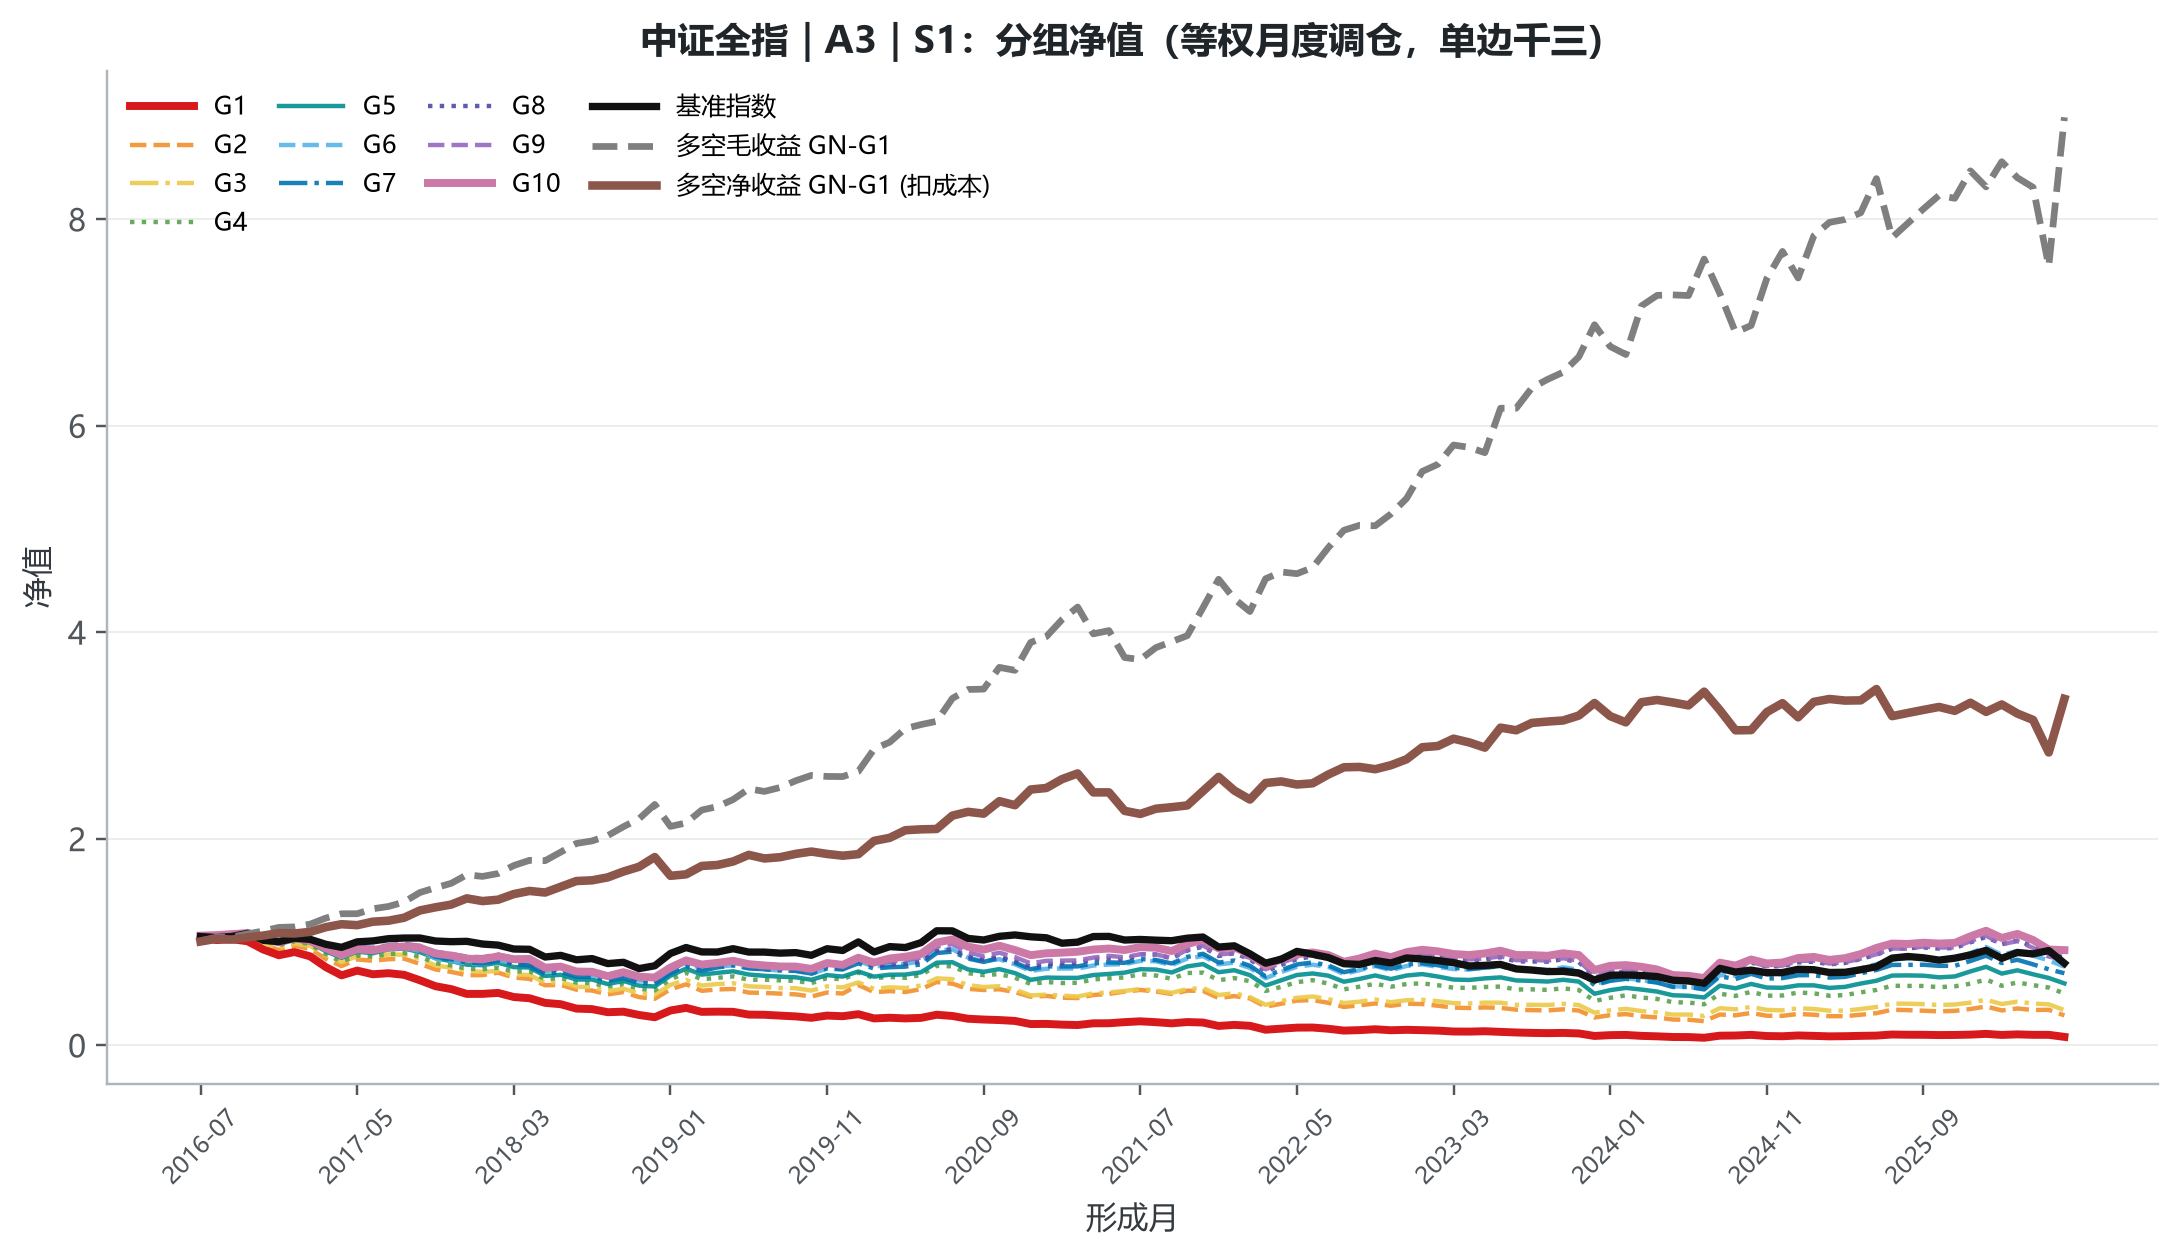
\includegraphics[width=\linewidth]{figs_v21/fig_5_2_zzall_A3_group_nav.png}
\vspace{2pt}\caption*{\textbf{\textcolor{reportred}{图 5-5}}　中证全指 / A3 / S1：分组净值（有效净多空 +12.87\%/年）}
\end{minipage}\hfill
\begin{minipage}[t]{0.49\textwidth}
\centering
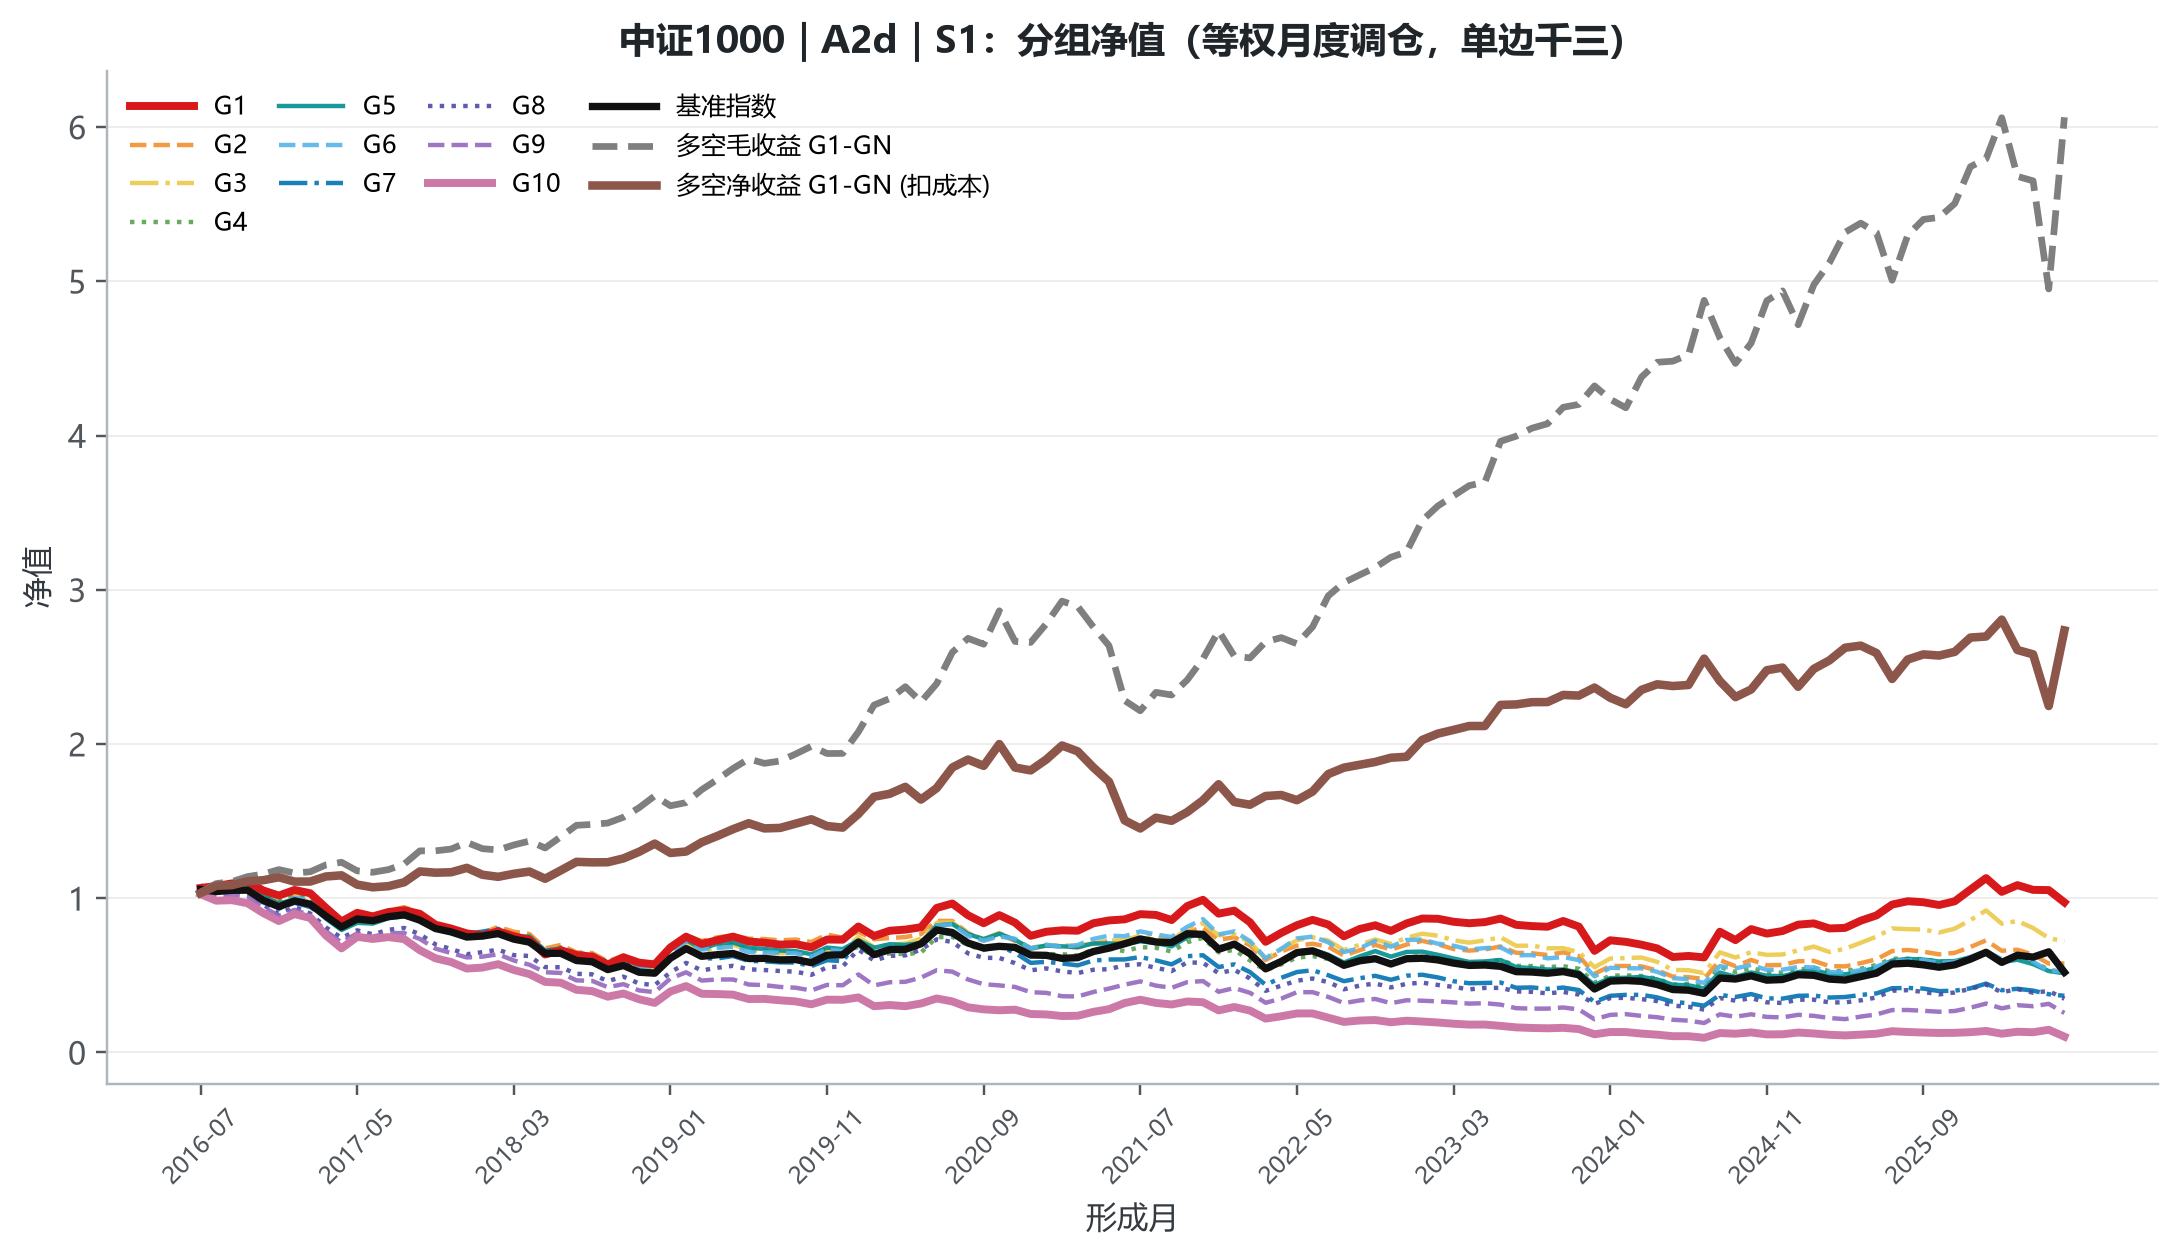
\includegraphics[width=\linewidth]{figs_v21/fig_5_3_zz1000_A2d_group_nav.png}
\vspace{2pt}\caption*{\textbf{\textcolor{reportred}{图 5-6}}　中证1000 / A2d / S1：分组净值（负向因子，取 $G\_1-G\_N$ 方向，有效净多空 +10.59\%/年）}
\end{minipage}
\end{figure}

\subsection{5.6
近期衰减：微观结构假设正在漂移}\label{ux8fd1ux671fux8870ux51cfux5faeux89c2ux7ed3ux6784ux5047ux8bbeux6b63ux5728ux6f02ux79fb}

以 A3 中证1000 为例，分年 IC 自 2017-2020 年的 4\%\textasciitilde10\%
降至 2024 年 3.6\%、2025 年 2.0\%、2026 上半年约
0；按固定的 \(G_N-G_1\) 方向并扣除双腿成本后，分年净多空由 2020 年 +53.1\%、2023 年 +12.3\% 降至 2025 年 −3.8\%。这一变化也与本体系其他因子（A2c 2025 年降至
0.7\%、B5a 2023
年后转正）互相印证。可能原因包括量化资金占比上升、程序化交易结构与撤单规则变化、以及
T+0
预期等制度因素------\textbf{微观结构类因子的假设环境漂移较快，失效区间（2020、2024-2025）的复盘与近期子样本监控应成为例行动作}。

为将单因子观察升级为全体系口径，本研究对全部 144
组回测补充统一的时间序列衰减分析（滚动 12/24 月 RankIC、前后半 ICIR
对比、2025 年以来子样本，与 §2.4/§3.4/§4.4
各因子后附的''时序衰减''同口径）。按''后半 \textbar ICIR\textbar{} −
前半 \textbar ICIR\textbar{}``排序，\textbf{衰减最重者集中于模块 B
的领先滞后族}（B5a 中证全指 −2.91→−0.21、B4 −4.10→−2.29、B3
−1.61→−0.07），其 alpha 在 2023 年后基本消失；模块 A 的 A3/A2c
幅度约减半但 2025 年以来月均 RankIC 仍 +6\%\textasciitilde+8\%（方向胜率
72\%\textasciitilde78\%），''衰减而未失效''；C3/A2a 则负向增强（C3
中证全指 −0.58→−1.87、A2a 沪深300
−0.05→−1.15）。\textbf{近期衰减并非均匀的 alpha
压缩，而是来源的结构性轮动}：领先滞后/确认度信息先被消化，而熵与高曲折时段的截面信息近一年反而增强。图
5-7 给出 18 因子 × 分年均值 RankIC 全景，可作为因子库例程监控的模板。

\begin{figure}[H]
\centering
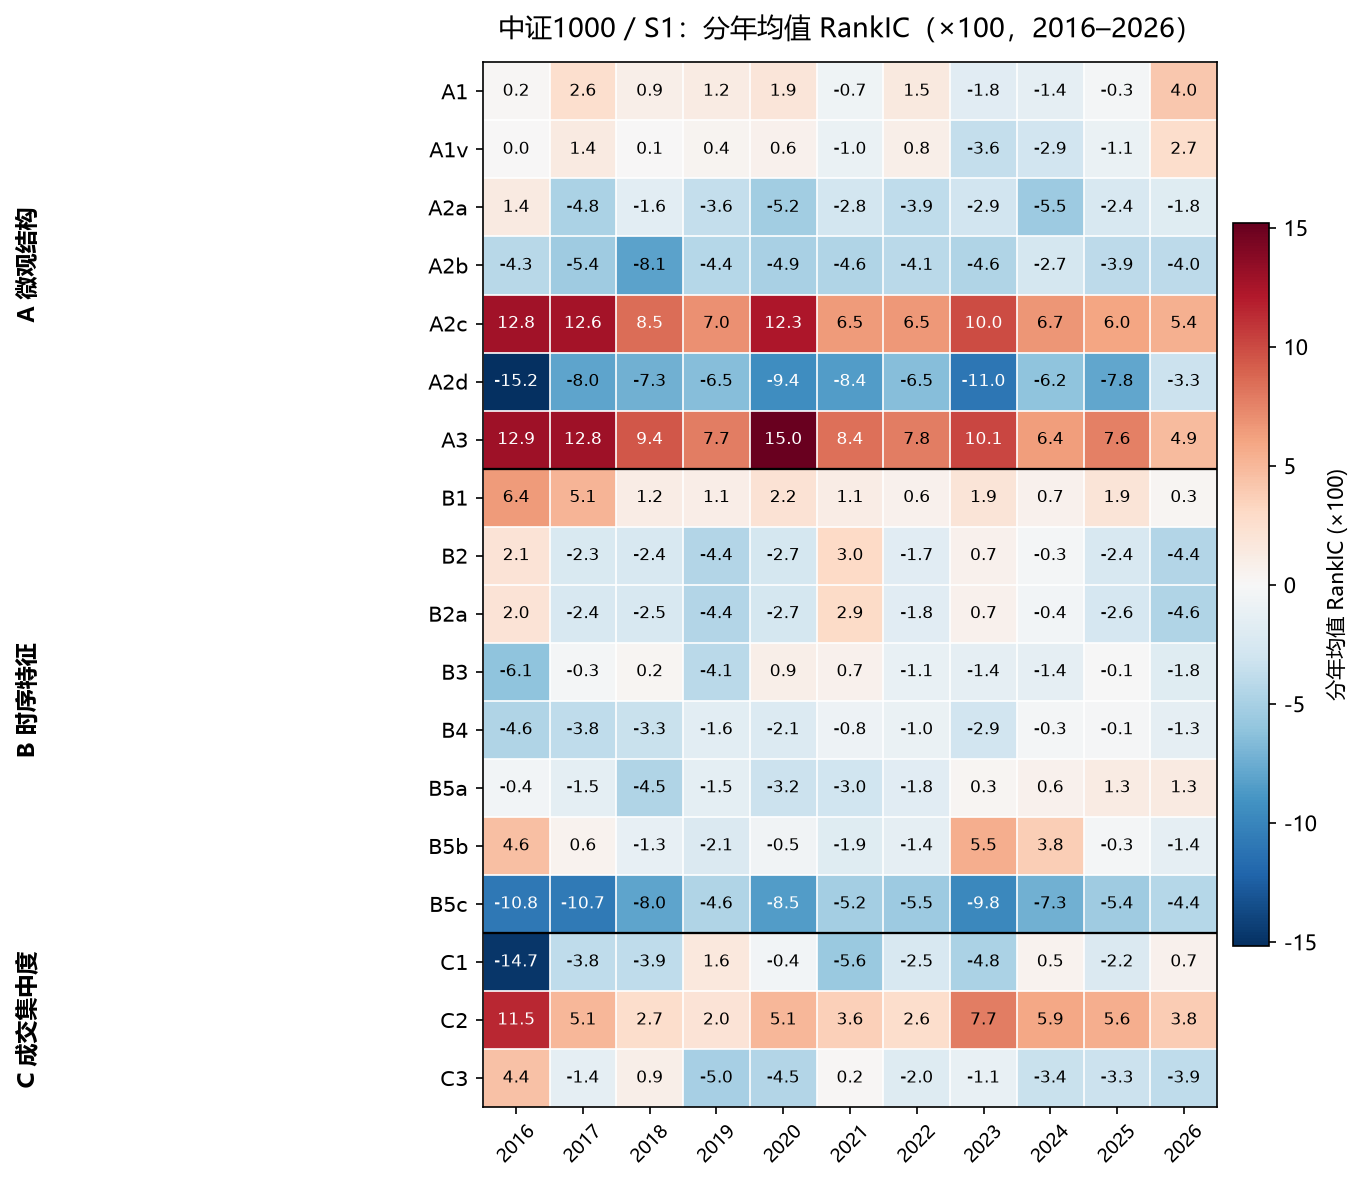
\includegraphics[width=.95\textwidth]{figs_v21/fig_5_7_zz1000_year_rankic_heatmap.png}
\caption*{\textbf{\textcolor{reportred}{图 5-7}}　中证1000 / S1：18 因子 × 分年均值 RankIC 全景热力图（×100；红正蓝负；2016/2026 各为 6 个月）}
\end{figure}

\subsection{5.7 方法论定位与本研究贡献}

本研究的方法论可以归纳为五点：
\begin{itemize}
\tightlist
\item \textbf{算子语法：}数据变换与 K 线聚合组成显式算子链，使因子定义与收益来源可以逐层追溯。
\item \textbf{时间段切割：}A2/A3/C2 以曲折度、放量或价格方向切分日内区间；只有能分离相反经济逻辑的切割才产生增量。
\item \textbf{时间点划分：}B5c 以累计收益新高为锚，比较锚点与非锚点量能；稀疏事件锚定优于对全日路径做无差别聚合。
\item \textbf{增量检验：}S1/S2/S3 逐层剥离市值、行业与九类风格；A3/A2c 部分借自量价风格，C2/B5c 更接近独立维度。
\item \textbf{时变检验：}前后半样本、滚动 RankIC 与近期子样本联合监控；不同收益来源发生结构性轮动，不能只看全样本均值。
\end{itemize}

本研究的主要贡献在于：将''路径曲折度''这一价格路径维度纳入时间段切割框架，并给出''\textbf{曲折度×成交量交叉（A3）}''与''\textbf{买卖两盘集中度差（C2）}''两个收益来源标签；同时以
144
组回测的完整对照，记录哪些切割有效、哪些无效，以及成本约束下真实可得的净收益。

\begin{center}\rule{0.5\linewidth}{0.5pt}\end{center}

\section{六、结论}\label{ux516dux7ed3ux8bba}

本研究以''数据变换---K线聚合''的统一语法，将日内价格路径的形态信息刻画为三个互补模块、18
个显式算子链因子，在十年期、四个股票池、两种中性化方案下完成 144
组回测。实证支持三条方法论命题：

\begin{enumerate}
\def\labelenumi{\arabic{enumi}.}
\tightlist
\item
  \textbf{结构优于总量。}
  日内定价效率不仅为总量指标（曲折度高低），更有时变结构------高曲折放量时段占比（A3）与成交集中度（A2c）为全体系最强因子，而总量（A1）信噪比最低。\textbf{切割与交叉是高频因子的主要增量来源}，但须选择能分离相反逻辑的切割维度。
\item
  \textbf{量价交互的方向性信息真实但需甄别。}
  ``先后''（B1，小盘有效）与''极值点''（B5c，顶背离反转、时序最稳）携带真实信息；``上下力量对比''（B2/B2a）与''斜率背离''（B5b）在月度频率上无效。\textbf{并非所有量价方向都值得构建因子。}
\item
  \textbf{量价中性是增量试金石，九风格全中性是最终检验。} 模块 A
  的强信号约一半借自波动率/换手率暴露（A3/A2c 的 S2 RankICIR
  约打对折），应作暴露管理；补全动量/反转/BP/DP/成长/盈利六风格后（S3）各因子几乎不再衰减，且
  C2（买卖盘集中度差）与 B5c 在完整九风格中性化下仍显著（中证全指 2.07 /
  −2.38），方为更接近独立维度的''干净增量''。
\item
  \textbf{因子效果在时间序列上呈结构性轮动。} 全量 144
  组的衰减分析（前后半 ICIR、滚动 RankIC、2025
  以来子样本）显示：领先滞后族（B3/B4/B5a）2023 年后基本消失，A3/A2c
  幅度减半但残差仍全体系最强，C3/A2a 负向增强------2025
  年以来的衰减是来源轮动而非均匀压缩，\textbf{2025
  以来子样本监控应成为因子库管理的例行动作}。
\end{enumerate}

同时，本研究诚实记录两个硬事实：\textbf{高频微观结构因子在 2025
年以来经历行业性衰减}（A3 分年 IC 2026
上半年趋零），以及\textbf{月度调仓下高换手对净收益的吞噬}（约一半毛信号让渡于成本）。\textbf{信号存在、来源可解释，但可交易性需要持有方案的工程改进}------拉长窗口降换手、阈值触发调仓、以及与低波/换手来源的暴露分离，为后续最值得投入的三个方向。这恰是收益来源导向研究的价值所在：\textbf{知道超额从何而来，也知道它在哪里会消失。}

\begin{center}\rule{0.5\linewidth}{0.5pt}\end{center}

\section{风险提示}\label{ux98ceux9669ux63d0ux793a}

\begin{enumerate}
\def\labelenumi{\arabic{enumi}.}
\tightlist
\item
  \textbf{模型存在失效风险}：市场的宏观环境与交易制度会随经济运行发生变化，若定价模式改变，或导致模型失效；
\item
  \textbf{市场交易行为发生变化}：影响以历史统计规律得到的因子的实际表现，2025
  年以来的衰减已现；
\item
  \textbf{历史回测不保证未来收益}：量化模型均基于历史数据回测，样本外数据分布与样本内可能存在较大差异；
\item
  \textbf{成本与冲击风险}：本报告按单边千三假设，实盘执行需另做交易成本与冲击成本评估；高换手方案下成本对净收益影响巨大。
\end{enumerate}

\begin{center}\rule{0.5\linewidth}{0.5pt}\end{center}

\section{附录：18 因子算子链速览（公式 +
聚合方式）}\label{ux9644ux5f5518-ux56e0ux5b50ux7b97ux5b50ux94feux901fux89c8ux516cux5f0f-ux805aux5408ux65b9ux5f0f}

\begin{longtable}[]{@{}
  >{\raggedright\arraybackslash}p{(\linewidth - 6\tabcolsep) * \real{0.2500}}
  >{\raggedright\arraybackslash}p{(\linewidth - 6\tabcolsep) * \real{0.2500}}
  >{\raggedright\arraybackslash}p{(\linewidth - 6\tabcolsep) * \real{0.2500}}
  >{\raggedright\arraybackslash}p{(\linewidth - 6\tabcolsep) * \real{0.2500}}@{}}
\caption{表 13　18 因子算子链速览}\tabularnewline
\toprule\noalign{}
\begin{minipage}[b]{\linewidth}\raggedright
因子（中文名）
\end{minipage} & \begin{minipage}[b]{\linewidth}\raggedright
代码
\end{minipage} & \begin{minipage}[b]{\linewidth}\raggedright
日度原子量公式
\end{minipage} & \begin{minipage}[b]{\linewidth}\raggedright
20 日聚合
\end{minipage} \\
\midrule\noalign{}
\endfirsthead
\toprule\noalign{}
\begin{minipage}[b]{\linewidth}\raggedright
因子（中文名）
\end{minipage} & \begin{minipage}[b]{\linewidth}\raggedright
代码
\end{minipage} & \begin{minipage}[b]{\linewidth}\raggedright
日度原子量公式
\end{minipage} & \begin{minipage}[b]{\linewidth}\raggedright
20 日聚合
\end{minipage} \\
\midrule\noalign{}
\endhead
\bottomrule\noalign{}
\endlastfoot
日内路径曲折度因子 & A1 &
\(\tau=\dfrac{\sum \lVert r_t\rVert}{\lVert\sum r_t\rVert+\varepsilon}\)
& 均值 \\
量加权路径曲折度因子 & A1v &
\(\tau_v=\dfrac{\sum \lVert r_t\rVert\cdot V_t/\bar V}{\lVert\sum r_t\rVert+\varepsilon}\)
& 均值 \\
高曲折时段价格噪音强度因子 & A2a & \(\sigma\big(\{r_t:d_t=1\}\big)\) &
均值 \\
低曲折时段信息驱动收益因子 & A2b & \(\sum_{d_t=0} r_t\) & 均值 \\
高曲折时段成交集中度因子 & A2c & \(\sum_{d_t=1} w_t\) & 均值 \\
高曲折时段换手强度因子 & A2d &
\(C_{\mathrm{high}}\times \mathrm{Turnover}\) & 均值 \\
曲折放量共振因子 & A3 &
\(\sum_t \mathbb{1}\{\tau^{(30)}_t>\mathrm{Med}\}\cdot\mathbb{1}\{V_t>\mu_V+\sigma_V\}/T_{\mathrm{win}}\)
& 均值 \\
量价领先滞后因子 & B1 &
\(\sum_k\frac1k\big(\rho(\Delta v_{t-k},r_t)-\rho(r_{t-k},\Delta v_t)\big)\)
& 均值 \\
上行路径量能不对称因子 & B2 &
\(PA=\dfrac{\sum_{r_t>0}a_tV_t}{\sum_{r_t<0}a_tV_t+\varepsilon}\) &
均值 \\
上行路径成交额不对称因子 & B2a & \(PA\)（量列换成
\(\mathrm{Amount}_t\)） & 均值 \\
方向条件化量价领先滞后因子 & B3 & \(LL^{+}-LL^{-}\)（按 \(r_t\)
符号条件化） & 均值 \\
量价力量动量交叉因子 & B4 & \((PA-1)\times LL\) & 均值 \\
日内量价确认度衰减因子 & B5a & \(\rho_{239}-\rho_{59}\)（60min
滚动量价相关） & 均值 \\
量价趋势斜率背离因子 & B5b & \(-\hat\beta_p^s\,\hat\beta_v^s\) & 均值 \\
价格新高量能不足因子 & B5c &
\(\dfrac{\mathrm{Mean}(V_t\mid h_t=1)}{\mathrm{Mean}(V_t\mid h_t=0)}\) &
均值 \\
日内成交集中度熵因子 & C1 & \(H^*=-\dfrac{\sum_t w_t\ln w_t}{\ln 240}\)
& 均值 \\
买卖盘成交集中度差异因子 & C2 & \(H^{+}-H^{-}\) & 均值 \\
成交集中度变异因子 & C3 & \(\mathrm{Std}_{20d}(H^*)\) &
\textbf{标准差} \\
\end{longtable}

\begin{center}\rule{0.5\linewidth}{0.5pt}\end{center}

\begin{quote}
\textbf{资料来源与可复现性}：全部因子、144 组回测与图表均由本研究基于 1
分钟 K 线独立实现；正式结果存于 \texttt{result/backtest\_v4}，数据规格、源码和环境说明随项目公开。

\textbf{风格数据}：量价类 5 风格由日频数据自建；BP、DP、盈利和成长按形成月末
point-in-time 对齐。本文仅作研究展示，不构成投资建议。
\end{quote}
\end{document}
